\documentclass[12pt]{cms-tdr}
\RCS$Revision: 1.0 $
\RCS$Date: Wed Sep 22 19:27:03 CDT 2010 $
\RCS$Name: Jim Pivarski $
%%%%%%%%%%%%%%%%%%%%%%%%%%%%%%%%%%%%%%%%%%%%%%%%%%%%%%%%%%%%%%%%%%%%
%
%  Common definitions
%
%  N.B. use of \providecommand rather than \newcommand means
%       that a definition is ignored if already specified
%
%                                              L. Taylor 18 Feb 2005
%%%%%%%%%%%%%%%%%%%%%%%%%%%%%%%%%%%%%%%%%%%%%%%%%%%%%%%%%%%%%%%%%%%%

% Some shorthand
% turn off italics
\newcommand {\etal}{\mbox{et al.}\xspace} %et al. - no preceding comma
\newcommand {\ie}{\mbox{i.e.}\xspace}     %i.e.
\newcommand {\eg}{\mbox{e.g.}\xspace}     %e.g.
\newcommand {\etc}{\mbox{etc.}\xspace}     %etc.
\newcommand {\vs}{\mbox{\sl vs.}\xspace}      %vs.
\newcommand {\mdash}{\ensuremath{\mathrm{-}}} % for use within formulas

% some terms whose definition we may change
\newcommand {\Lone}{Level-1\xspace} % Level-1 or L1 ?
\newcommand {\Ltwo}{Level-2\xspace}
\newcommand {\Lthree}{Level-3\xspace}

% Some software programs (alphabetized)
\providecommand{\ACERMC} {\textsc{AcerMC}\xspace}
\providecommand{\ALPGEN} {{\textsc{alpgen}}\xspace}
\providecommand{\CHARYBDIS} {{\textsc{charybdis}}\xspace}
\providecommand{\CMKIN} {\textsc{cmkin}\xspace}
\providecommand{\CMSIM} {{\textsc{cmsim}}\xspace}
\providecommand{\CMSSW} {{\textsc{cmssw}}\xspace}
\providecommand{\COBRA} {{\textsc{cobra}}\xspace}
\providecommand{\COCOA} {{\textsc{cocoa}}\xspace}
\providecommand{\COMPHEP} {\textsc{CompHEP}\xspace}
\providecommand{\EVTGEN} {{\textsc{evtgen}}\xspace}
\providecommand{\FAMOS} {{\textsc{famos}}\xspace}
\providecommand{\GARCON} {\textsc{garcon}\xspace}
\providecommand{\GARFIELD} {{\textsc{garfield}}\xspace}
\providecommand{\GEANE} {{\textsc{geane}}\xspace}
\providecommand{\GEANTfour} {{\textsc{geant4}}\xspace}
\providecommand{\GEANTthree} {{\textsc{geant3}}\xspace}
\providecommand{\GEANT} {{\textsc{geant}}\xspace}
\providecommand{\HDECAY} {\textsc{hdecay}\xspace}
\providecommand{\HERWIG} {{\textsc{herwig}}\xspace}
\providecommand{\HIGLU} {{\textsc{higlu}}\xspace}
\providecommand{\HIJING} {{\textsc{hijing}}\xspace}
\providecommand{\IGUANA} {\textsc{iguana}\xspace}
\providecommand{\ISAJET} {{\textsc{isajet}}\xspace}
\providecommand{\ISAPYTHIA} {{\textsc{isapythia}}\xspace}
\providecommand{\ISASUGRA} {{\textsc{isasugra}}\xspace}
\providecommand{\ISASUSY} {{\textsc{isasusy}}\xspace}
\providecommand{\ISAWIG} {{\textsc{isawig}}\xspace}
\providecommand{\MADGRAPH} {\textsc{MadGraph}\xspace}
\providecommand{\MCATNLO} {\textsc{mc@nlo}\xspace}
\providecommand{\MCFM} {\textsc{mcfm}\xspace}
\providecommand{\MILLEPEDE} {{\textsc{millepede}}\xspace}
\providecommand{\ORCA} {{\textsc{orca}}\xspace}
\providecommand{\OSCAR} {{\textsc{oscar}}\xspace}
\providecommand{\PHOTOS} {\textsc{photos}\xspace}
\providecommand{\PROSPINO} {\textsc{prospino}\xspace}
\providecommand{\PYTHIA} {{\textsc{pythia}}\xspace}
\providecommand{\SHERPA} {{\textsc{sherpa}}\xspace}
\providecommand{\TAUOLA} {\textsc{tauola}\xspace}
\providecommand{\TOPREX} {\textsc{TopReX}\xspace}
\providecommand{\XDAQ} {{\textsc{xdaq}}\xspace}


%  Experiments
\newcommand {\DZERO}{D\O\xspace}     %etc.


% Measurements and units...

\newcommand{\de}{\ensuremath{^\circ}}
\newcommand{\ten}[1]{\ensuremath{\times \text{10}^\text{#1}}}
\newcommand{\unit}[1]{\ensuremath{\text{\,#1}}\xspace}
\newcommand{\mum}{\ensuremath{\,\mu\text{m}}\xspace}
\newcommand{\micron}{\ensuremath{\,\mu\text{m}}\xspace}
\newcommand{\cm}{\ensuremath{\,\text{cm}}\xspace}
\newcommand{\mm}{\ensuremath{\,\text{mm}}\xspace}
\newcommand{\mus}{\ensuremath{\,\mu\text{s}}\xspace}
\newcommand{\keV}{\ensuremath{\,\text{ke\hspace{-.08em}V}}\xspace}
\newcommand{\MeV}{\ensuremath{\,\text{Me\hspace{-.08em}V}}\xspace}
\newcommand{\GeV}{\ensuremath{\,\text{Ge\hspace{-.08em}V}}\xspace}
\newcommand{\TeV}{\ensuremath{\,\text{Te\hspace{-.08em}V}}\xspace}
\newcommand{\PeV}{\ensuremath{\,\text{Pe\hspace{-.08em}V}}\xspace}
\newcommand{\keVc}{\ensuremath{{\,\text{ke\hspace{-.08em}V\hspace{-0.16em}/\hspace{-0.08em}}c}}\xspace}
\newcommand{\MeVc}{\ensuremath{{\,\text{Me\hspace{-.08em}V\hspace{-0.16em}/\hspace{-0.08em}}c}}\xspace}
\newcommand{\GeVc}{\ensuremath{{\,\text{Ge\hspace{-.08em}V\hspace{-0.16em}/\hspace{-0.08em}}c}}\xspace}
\newcommand{\TeVc}{\ensuremath{{\,\text{Te\hspace{-.08em}V\hspace{-0.16em}/\hspace{-0.08em}}c}}\xspace}
\newcommand{\keVcc}{\ensuremath{{\,\text{ke\hspace{-.08em}V\hspace{-0.16em}/\hspace{-0.08em}}c^\text{2}}}\xspace}
\newcommand{\MeVcc}{\ensuremath{{\,\text{Me\hspace{-.08em}V\hspace{-0.16em}/\hspace{-0.08em}}c^\text{2}}}\xspace}
\newcommand{\GeVcc}{\ensuremath{{\,\text{Ge\hspace{-.08em}V\hspace{-0.16em}/\hspace{-0.08em}}c^\text{2}}}\xspace}
\newcommand{\TeVcc}{\ensuremath{{\,\text{Te\hspace{-.08em}V\hspace{-0.16em}/\hspace{-0.08em}}c^\text{2}}}\xspace}

\newcommand{\pbinv} {\mbox{\ensuremath{\,\text{pb}^\text{$-$1}}}\xspace}
\newcommand{\fbinv} {\mbox{\ensuremath{\,\text{fb}^\text{$-$1}}}\xspace}
\newcommand{\nbinv} {\mbox{\ensuremath{\,\text{nb}^\text{$-$1}}}\xspace}
\newcommand{\percms}{\ensuremath{\,\text{cm}^\text{$-$2}\,\text{s}^\text{$-$1}}\xspace}
\newcommand{\lumi}{\ensuremath{\mathcal{L}}\xspace}
\newcommand{\Lumi}{\ensuremath{\mathcal{L}}\xspace}%both upper and lower
%
% Need a convention here:
\newcommand{\LvLow}  {\ensuremath{\mathcal{L}=\text{10}^\text{32}\,\text{cm}^\text{$-$2}\,\text{s}^\text{$-$1}}\xspace}
\newcommand{\LLow}   {\ensuremath{\mathcal{L}=\text{10}^\text{33}\,\text{cm}^\text{$-$2}\,\text{s}^\text{$-$1}}\xspace}
\newcommand{\lowlumi}{\ensuremath{\mathcal{L}=\text{2}\times \text{10}^\text{33}\,\text{cm}^\text{$-$2}\,\text{s}^\text{$-$1}}\xspace}
\newcommand{\LMed}   {\ensuremath{\mathcal{L}=\text{2}\times \text{10}^\text{33}\,\text{cm}^\text{$-$2}\,\text{s}^\text{$-$1}}\xspace}
\newcommand{\LHigh}  {\ensuremath{\mathcal{L}=\text{10}^\text{34}\,\text{cm}^\text{-2}\,\text{s}^\text{$-$1}}\xspace}
\newcommand{\hilumi} {\ensuremath{\mathcal{L}=\text{10}^\text{34}\,\text{cm}^\text{-2}\,\text{s}^\text{$-$1}}\xspace}

% Some usual physics terms

\newcommand{\zp}{\ensuremath{\mathrm{Z}^\prime}\xspace}

% SM (still to be classified)

\newcommand{\kt}{\ensuremath{k_{\mathrm{T}}}\xspace}
\newcommand{\BC}{\ensuremath{{B_{\mathrm{c}}}}\xspace}
\newcommand{\bbarc}{\ensuremath{{\overline{b}c}}\xspace}
\newcommand{\bbbar}{\ensuremath{{b\overline{b}}}\xspace}
\newcommand{\ccbar}{\ensuremath{{c\overline{c}}}\xspace}
\newcommand{\JPsi}{\ensuremath{{J}\hspace{-.08em}/\hspace{-.14em}\psi}\xspace}
\newcommand{\bspsiphi}{\ensuremath{B_s \to \JPsi\, \phi}\xspace}
%\newcommand{\ttbar}{\ensuremath{{t\overline{t}}}\xspace}
\newcommand{\AFB}{\ensuremath{A_\text{FB}}\xspace}
\newcommand{\EE}{\ensuremath{e^+e^-}\xspace}
\newcommand{\MM}{\ensuremath{\mu^+\mu^-}\xspace}
\newcommand{\TT}{\ensuremath{\tau^+\tau^-}\xspace}
\newcommand{\wangle}{\ensuremath{\sin^{2}\theta_{\text{eff}}^\text{lept}(M^2_\mathrm{Z})}\xspace}
\newcommand{\ttbar}{\ensuremath{{t\overline{t}}}\xspace}
\newcommand{\stat}{\ensuremath{\,\text{(stat.)}}\xspace}
\newcommand{\syst}{\ensuremath{\,\text{(syst.)}}\xspace}
% these moved to similar defs
%\newcommand{\Etmiss}{\ensuremath{E_{\mathrm{T}\!{\rm miss}}}}
%\newcommand{\VEtmiss}{\ensuremath{{\vec E}_{\mathrm{T}\!{\rm miss}}}}

%%%  E-gamma definitions
\newcommand{\HGG}{\ensuremath{\mathrm{H}\to\gamma\gamma}}
\newcommand{\gev}{\GeV}
\newcommand{\GAMJET}{\ensuremath{\gamma + \text{jet}}}
\newcommand{\PPTOJETS}{\ensuremath{\mathrm{pp}\to\text{jets}}}
\newcommand{\PPTOGG}{\ensuremath{\mathrm{pp}\to\gamma\gamma}}
\newcommand{\PPTOGAMJET}{\ensuremath{\mathrm{pp}\to\gamma +
\mathrm{jet}
}}
\newcommand{\MH}{\ensuremath{\mathrm{M_{\mathrm{H}}}}}
\newcommand{\RNINE}{\ensuremath{\mathrm{R}_\mathrm{9}}}
\newcommand{\DR}{\ensuremath{\Delta\mathrm{R}}}



% Physics symbols ...

\newcommand{\PT}{\ensuremath{p_{\mathrm{T}}}\xspace}
\newcommand{\pt}{\ensuremath{p_{\mathrm{T}}}\xspace}
\newcommand{\ET}{\ensuremath{E_{\mathrm{T}}}\xspace}
\newcommand{\HT}{\ensuremath{H_{\mathrm{T}}}\xspace}
\newcommand{\et}{\ensuremath{E_{\mathrm{T}}}\xspace}
\newcommand{\Em}{\ensuremath{E\!\!\!/}\xspace}
\newcommand{\Pm}{\ensuremath{p\!\!\!/}\xspace}
\newcommand{\PTm}{\ensuremath{{p\!\!\!/}_{\mathrm{T}}}\xspace}
\newcommand{\ETm}{\ensuremath{E_{\mathrm{T}}^{\text{miss}}}\xspace}
\newcommand{\MET}{\ensuremath{E_{\mathrm{T}}^{\text{miss}}}\xspace}
\newcommand{\ETmiss}{\ensuremath{E_{\mathrm{T}}^{\text{miss}}}\xspace}
\newcommand{\VEtmiss}{\ensuremath{{\vec E}_{\mathrm{T}}^{\text{miss}}}\xspace}

%%%%%%
% From Albert
%

\newcommand{\ga}{\ensuremath{\gtrsim}}
\newcommand{\la}{\ensuremath{\lesssim}}
%\def\ga{\mathrel{\rlap{\raise.6ex\hbox{$>$}}{\lower.6ex\hbox{$\sim$}}}}
%\def\la{\mathrel{\rlap{\raise.6ex\hbox{$<$}}{\lower.6ex\hbox{$\sim$}}}}
%
\newcommand{\swsq}{\ensuremath{\sin^2\theta_W}\xspace}
\newcommand{\cwsq}{\ensuremath{\cos^2\theta_W}\xspace}
\newcommand{\tanb}{\ensuremath{\tan\beta}\xspace}
\newcommand{\tanbsq}{\ensuremath{\tan^{2}\beta}\xspace}
\newcommand{\sidb}{\ensuremath{\sin 2\beta}\xspace}
\newcommand{\alpS}{\ensuremath{\alpha_S}\xspace}
\newcommand{\alpt}{\ensuremath{\tilde{\alpha}}\xspace}

\newcommand{\QL}{\ensuremath{Q_L}\xspace}
\newcommand{\sQ}{\ensuremath{\tilde{Q}}\xspace}
\newcommand{\sQL}{\ensuremath{\tilde{Q}_L}\xspace}
\newcommand{\ULC}{\ensuremath{U_L^C}\xspace}
\newcommand{\sUC}{\ensuremath{\tilde{U}^C}\xspace}
\newcommand{\sULC}{\ensuremath{\tilde{U}_L^C}\xspace}
\newcommand{\DLC}{\ensuremath{D_L^C}\xspace}
\newcommand{\sDC}{\ensuremath{\tilde{D}^C}\xspace}
\newcommand{\sDLC}{\ensuremath{\tilde{D}_L^C}\xspace}
\newcommand{\LL}{\ensuremath{L_L}\xspace}
\newcommand{\sL}{\ensuremath{\tilde{L}}\xspace}
\newcommand{\sLL}{\ensuremath{\tilde{L}_L}\xspace}
\newcommand{\ELC}{\ensuremath{E_L^C}\xspace}
\newcommand{\sEC}{\ensuremath{\tilde{E}^C}\xspace}
\newcommand{\sELC}{\ensuremath{\tilde{E}_L^C}\xspace}
\newcommand{\sEL}{\ensuremath{\tilde{E}_L}\xspace}
\newcommand{\sER}{\ensuremath{\tilde{E}_R}\xspace}
\newcommand{\sFer}{\ensuremath{\tilde{f}}\xspace}
\newcommand{\sQua}{\ensuremath{\tilde{q}}\xspace}
\newcommand{\sUp}{\ensuremath{\tilde{u}}\xspace}
\newcommand{\suL}{\ensuremath{\tilde{u}_L}\xspace}
\newcommand{\suR}{\ensuremath{\tilde{u}_R}\xspace}
\newcommand{\sDw}{\ensuremath{\tilde{d}}\xspace}
\newcommand{\sdL}{\ensuremath{\tilde{d}_L}\xspace}
\newcommand{\sdR}{\ensuremath{\tilde{d}_R}\xspace}
\newcommand{\sTop}{\ensuremath{\tilde{t}}\xspace}
\newcommand{\stL}{\ensuremath{\tilde{t}_L}\xspace}
\newcommand{\stR}{\ensuremath{\tilde{t}_R}\xspace}
\newcommand{\stone}{\ensuremath{\tilde{t}_1}\xspace}
\newcommand{\sttwo}{\ensuremath{\tilde{t}_2}\xspace}
\newcommand{\sBot}{\ensuremath{\tilde{b}}\xspace}
\newcommand{\sbL}{\ensuremath{\tilde{b}_L}\xspace}
\newcommand{\sbR}{\ensuremath{\tilde{b}_R}\xspace}
\newcommand{\sbone}{\ensuremath{\tilde{b}_1}\xspace}
\newcommand{\sbtwo}{\ensuremath{\tilde{b}_2}\xspace}
\newcommand{\sLep}{\ensuremath{\tilde{l}}\xspace}
\newcommand{\sLepC}{\ensuremath{\tilde{l}^C}\xspace}
\newcommand{\sEl}{\ensuremath{\tilde{e}}\xspace}
\newcommand{\sElC}{\ensuremath{\tilde{e}^C}\xspace}
\newcommand{\seL}{\ensuremath{\tilde{e}_L}\xspace}
\newcommand{\seR}{\ensuremath{\tilde{e}_R}\xspace}
\newcommand{\snL}{\ensuremath{\tilde{\nu}_L}\xspace}
\newcommand{\sMu}{\ensuremath{\tilde{\mu}}\xspace}
\newcommand{\sNu}{\ensuremath{\tilde{\nu}}\xspace}
\newcommand{\sTau}{\ensuremath{\tilde{\tau}}\xspace}
\newcommand{\Glu}{\ensuremath{g}\xspace}
\newcommand{\sGlu}{\ensuremath{\tilde{g}}\xspace}
\newcommand{\Wpm}{\ensuremath{W^{\pm}}\xspace}
\newcommand{\sWpm}{\ensuremath{\tilde{W}^{\pm}}\xspace}
\newcommand{\Wz}{\ensuremath{W^{0}}\xspace}
\newcommand{\sWz}{\ensuremath{\tilde{W}^{0}}\xspace}
\newcommand{\sWino}{\ensuremath{\tilde{W}}\xspace}
\newcommand{\Bz}{\ensuremath{B^{0}}\xspace}
\newcommand{\sBz}{\ensuremath{\tilde{B}^{0}}\xspace}
\newcommand{\sBino}{\ensuremath{\tilde{B}}\xspace}
\newcommand{\Zz}{\ensuremath{Z^{0}}\xspace}
\newcommand{\sZino}{\ensuremath{\tilde{Z}^{0}}\xspace}
\newcommand{\sGam}{\ensuremath{\tilde{\gamma}}\xspace}
\newcommand{\chiz}{\ensuremath{\tilde{\chi}^{0}}\xspace}
\newcommand{\chip}{\ensuremath{\tilde{\chi}^{+}}\xspace}
\newcommand{\chim}{\ensuremath{\tilde{\chi}^{-}}\xspace}
\newcommand{\chipm}{\ensuremath{\tilde{\chi}^{\pm}}\xspace}
\newcommand{\Hone}{\ensuremath{H_{d}}\xspace}
\newcommand{\sHone}{\ensuremath{\tilde{H}_{d}}\xspace}
\newcommand{\Htwo}{\ensuremath{H_{u}}\xspace}
\newcommand{\sHtwo}{\ensuremath{\tilde{H}_{u}}\xspace}
\newcommand{\sHig}{\ensuremath{\tilde{H}}\xspace}
\newcommand{\sHa}{\ensuremath{\tilde{H}_{a}}\xspace}
\newcommand{\sHb}{\ensuremath{\tilde{H}_{b}}\xspace}
\newcommand{\sHpm}{\ensuremath{\tilde{H}^{\pm}}\xspace}
\newcommand{\hz}{\ensuremath{h^{0}}\xspace}
\newcommand{\Hz}{\ensuremath{H^{0}}\xspace}
\newcommand{\Az}{\ensuremath{A^{0}}\xspace}
\newcommand{\Hpm}{\ensuremath{H^{\pm}}\xspace}
\newcommand{\sGra}{\ensuremath{\tilde{G}}\xspace}
%
\newcommand{\mtil}{\ensuremath{\tilde{m}}\xspace}
%
\newcommand{\rpv}{\ensuremath{\rlap{\kern.2em/}R}\xspace}
\newcommand{\LLE}{\ensuremath{LL\bar{E}}\xspace}
\newcommand{\LQD}{\ensuremath{LQ\bar{D}}\xspace}
\newcommand{\UDD}{\ensuremath{\overline{UDD}}\xspace}
\newcommand{\Lam}{\ensuremath{\lambda}\xspace}
\newcommand{\Lamp}{\ensuremath{\lambda'}\xspace}
\newcommand{\Lampp}{\ensuremath{\lambda''}\xspace}
%
\newcommand{\spinbd}[2]{\ensuremath{\bar{#1}_{\dot{#2}}}\xspace}

\newcommand{\MD}{\ensuremath{{M_\mathrm{D}}}\xspace}% ED mass
\newcommand{\Mpl}{\ensuremath{{M_\mathrm{Pl}}}\xspace}% Planck mass
\newcommand{\Rinv} {\ensuremath{{R}^{-1}}\xspace}



%%%%%%%%%%%%%%%%%%%%%%%%%%%%%%%%%%%%%%%%%%%%%%%%%%%%%%%%%%%%%%%%%%%%
%
% Hyphenations (only need to add here if you get a nasty word break)
%
\hyphenation{en-viron-men-tal}%    just an example

\cmsNoteHeader{EXO-10-999}

\newcommand{\s}[1]{{\mbox{\scriptsize #1}}}

\textheight=8.5 in

\title{Search for Collimated Groups of Muons}
\author{Jim Pivarski, Alexei Safonov, Aysen Tatarinov}
\date{\today}

\abstract{We present an inclusive, signature-based search for groups
  of collimated muons, arising from spectroscopic cascades in a hidden
  sector accessible only through high-energy collisions, using the CMS
  detector.  In several signatures defined by number of muons per
  collimated group and number of groups per event, we searched for the
  lightest on-shell state in the hidden spectrum with a mass-peak fit and set
  limits on $\sigma\mathcal{B}\alpha$, where $\alpha$ is the model
  acceptance of the signature.  Depending on the signature and the
  mass of the lightest state ($2m_\mu$--5~GeV/$c^2$), new resonances
  are ruled out at the level of $XX$-$YY$~pb for 95\% C.L.  We also
  set $\sigma\mathcal{B}$ limits on two representative benchmark
  models: SUSY dark matter with a $\mathcal{U}(1)_\s{dark}$ and NMSSM
  Higgs escaping LEP limits via Higgs-to-Higgs decays. \vspace{0.5
    cm}}

\hypersetup{%
pdfauthor={CMS Collaboration},%
pdftitle={Search for Collimated Groups of Muons},%
pdfsubject={CMS},%
pdfkeywords={CMS, physics, exotica, muons}}

\begin{document}
\maketitle

\section{Introduction}

\subsection{Motivation}

\fixme{Needs a lot of references.}

Although the dimuon mass spectrum is well understood in $e^+e^-$ and
$p\bar{p}$ collisions up to collision energies of 0.2 and 2~TeV
respectively, (\fixme{get real numbers}) new states may be hidden by
weak couplings to Standard Model particles.  A wide class of
hidden-valley models predicts new states coupling weakly to the
Standard Model yet significantly to a hidden sector, accessible to the
LHC through massive particles that connect the two sectors.  In these
scenarios, massive particles $M$ would be created singly or in pairs
and then decay through the hidden spectrum to the lightest hidden
state: $pp \to M\overline{M}$ and $M \to m X$ where $m$ is the
lightest hidden particle.  If $m$ is unstable, it would decay with
very small width to the kinematically-accessible Standard Model
states, either democratically ($Z$-like) or to the heaviest accessible
state (Higgs-like).  Muon-pair final states would appear as a
low-mass, high-momentum dimuon resonance, and therefore be collimated
by relativistic boost.  With several low-mass states in the decay
chain, e.g.\ $m_2 \to m_1 m_1 \to 4\mu$, cascades would either produce
two groups of collimated dimuons or one group of four collimated
muons, depending on the boost of $m_2$.  Arbitrarily complex decay
chains are conceivable, and groups of muons might be produced in
association with other Standard Model pairs, such as $e^+e^-$ and
$\pi\pi$.  These striking signatures are often called ``lepton jets.''

Hidden, low-mass resonances are especially interesting in light of the
high-energy positron excess reported by the PAMELA primary cosmic-ray
experiment.  This excess of interstellar positrons could be the
product of WIMP annihilations, assuming that the WIMP annihilation
rate is higher than what would be expected from thermal freeze-out in
the early universe, and also assuming some mechanism to prohibit decay
chains that produce antiprotons, in which no excess was observed.  A
new force boson, $z_\s{dark}$, with a mass of approximately
1~GeV/$c^2$ and coupling significantly to WIMPs yet weakly to Standard
Model particles, would explain both observations.  Acting as a
long-range Yukawa force, $z_\s{dark}$ would draw together slow-moving
WIMPs, increasing their effective annihilation cross-section in the
modern era without affecting their production in the early universe.
As a decay channel, $z_\s{dark} \to p\bar{p} X$ would be kinematically
forbidden if the mass of $z_\s{dark}$ were above 2~GeV/$c^2$ or so.
Relatively simple extensions of this picture, such as adding a dark
Higgs boson $h_\s{dark}$ to give the $z_\s{dark}$ its mass, or
introducing the force with non-abelian structure, would produce more
complex event topologies: $2^N$ fermion pairs per lepton jet for a
two-body decay chain with $N$ light states and/or several lepton jets
per event if the decay chain includes heavy particles.

Another, very different, motivation derives from the tension between
the low Higgs mass predicted by precision electroweak fits and the
direct LEP limit of 114~GeV/$c^2$.  This limit assumes that the Higgs
boson decays directly into Standard Model particles with known
branching fractions.  If additional light Higgs bosons allow for
Higgs-to-Higgs decays, the direct limit may be circumvented.  In a
well-defined region of Next-to Minimal SuperSymmetric (NMSSM)
parameter space, the lightest CP-odd Higgs ($a_1$) can have
arbitrarily low mass.  Below the $2m_\tau$ threshold, the branching
fraction for $a_1 \to \mu\mu$ is about 20\%, making its detection in
the muon channel visible.  For values of the NMSSM parameters that
give the lightest CP-even Higgs ($h_1$) a large singlet field
component, $h_1 \to a_1 a_1$ can be as large as 100\%.  If nature has
chosen this model, then the Higgs mass could be as low as 86~GeV/$c^2$
and the primary Higgs signature would be $h_1 \to a_1 a_1 \to 2\mu,
2\mu$, where the dimuons appear as well-collimated lepton jets.

\subsection{Analysis Strategy}

\fixme{Shorten: should explain categoriziation, fundamental dimuons
  (closest in mass), got shapes from data, fit to floating combination
  of data and background}

In this paper, we present an inclusive, signature-based search for
collimated dimuons with a $2m_\mu$--$5$~GeV/$c^2$
resonance peak arising from hidden, on-shell cascade chains.
Additional objects, such as isolated single leptons, hadronic jets,
and missing energy, are neither included in the search nor are they
forbidden.  In particular, boosted dimuons are not rejected if they
are overlapped by $e^+e^-$ or $\pi\pi$ from other resonance decays in
the same lepton jet, nor are they rejected due to activity from a
nearby hadronic jet that might arise, for example, from cascades of
supersymmetric particles.

We assume that all decay chains in the hidden sector reach an on-shell
lowest-mass state $m_1$ before decaying to opposite-sign muon pairs,
though there may be several instances of this particle per event,
possibly overlapping one another (Fig.~\ref{fig:basic_picture}).  This
assumption is equivalent to assuming that the coupling between the
hidden states and the Standard Model is much weaker than the couplings
of the hidden states with each other, and the spectrum of heavy states
is not highly degenerate.  We therefore search for one new resonance
with a single dimuon mass peak, after identifying the combination of
muon pairs that is most likely to have arisen from distinct resonance
decays.

\begin{figure}
\mbox{ } \hfill 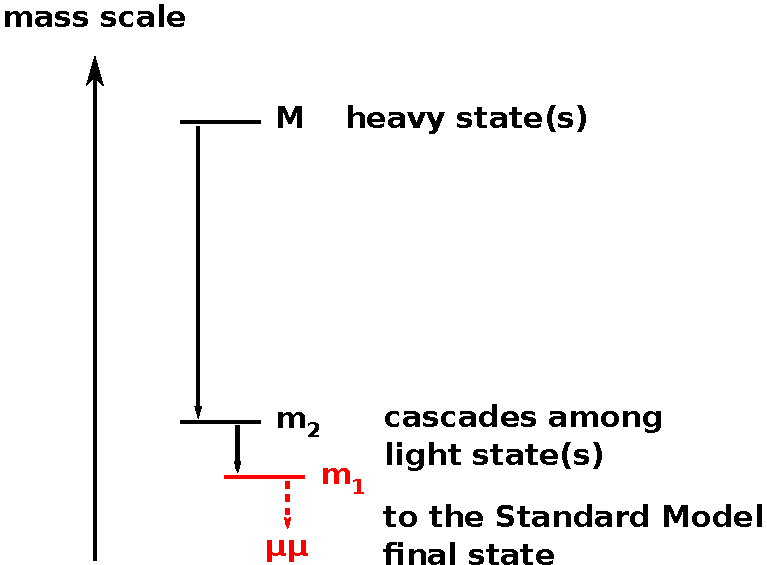
\includegraphics[width=0.45\linewidth]{PLOTS/basic_picture4.pdf} \hfill
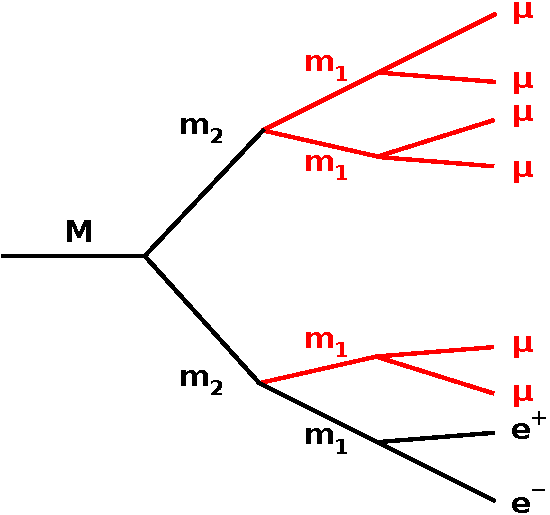
\includegraphics[width=0.35\linewidth]{PLOTS/basic_picture5.pdf} \hfill \mbox{ }

\caption{Schematic of a decay chain from heavy states in the hidden
  sector to light states, ultimately to Standard Model pairs.  We
  identify groups of muons collimated by boost, possibly containing
  non-muons and search for a resonance in muon pairs from $m_1 \to
  \mu\mu$. \label{fig:basic_picture}}
\end{figure}

Identifying the distinct dimuon resonances proceeds in two steps.
First, nearby muons are grouped into ``mu-jets'' with an arbitrary
number of muons per group.  The definition of ``nearby muons'' is
kinematic rather than geometric: two muons are considered near each
other if their pairwise invariant mass is less than 5~GeV/$c^2$ with
both muons satisfying a minimim-$p_T$ threshold.  This differs from
selections based on a maximum $\Delta R = \sqrt{(\Delta \phi)^2 +
  (\Delta \eta)^2}$ because $\Delta R$ approximately corresponds to
relativistic boost, effectively a tighter requirement on resonance
momentum for higher resonance masses (see
Fig.~\ref{fig:openingangle_dr}).

\begin{figure}
\begin{center}
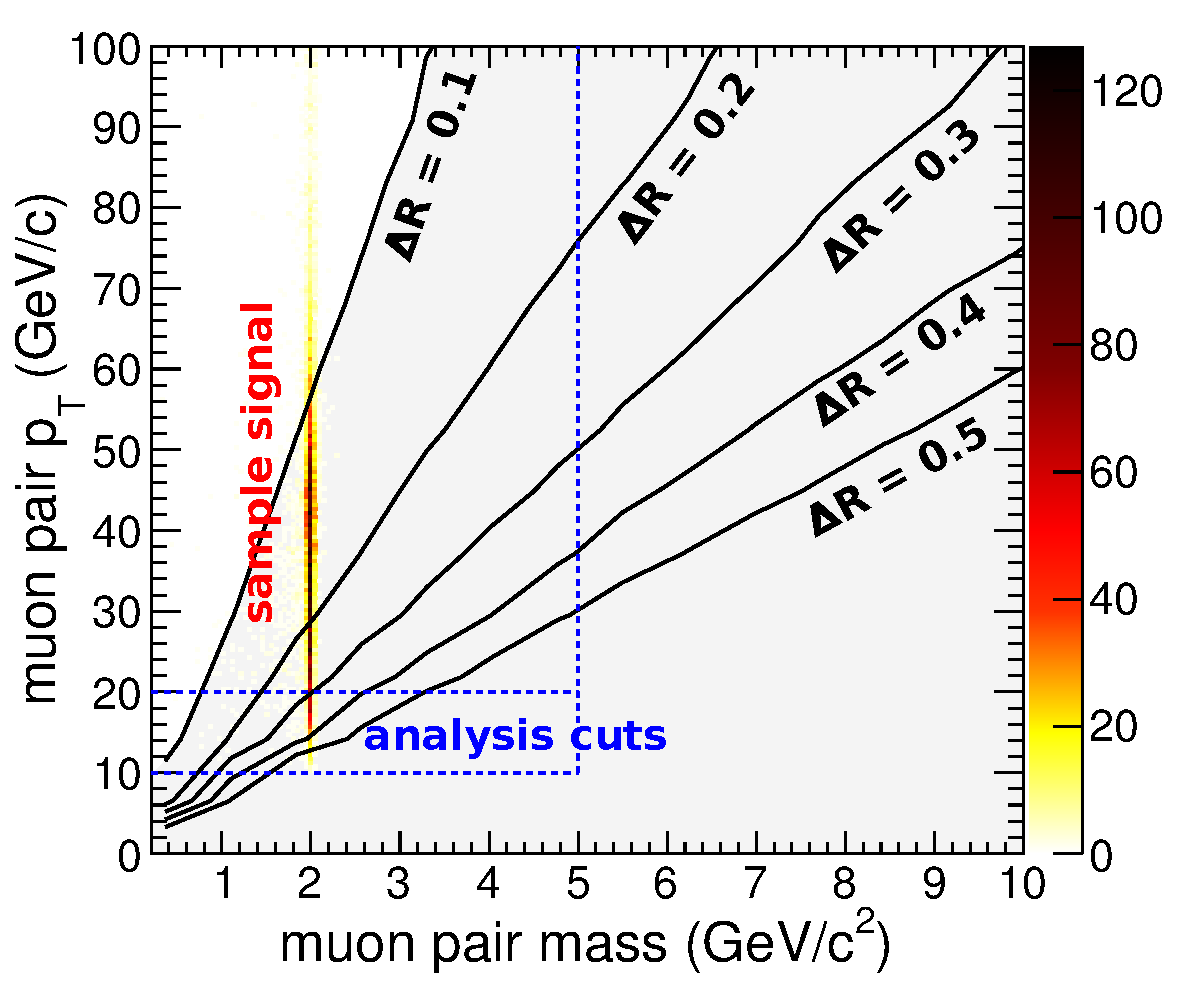
\includegraphics[width=0.65\linewidth]{PLOTS/openingangle_with_signal.pdf}
\end{center}

\caption{Sample signal (NMSSM with $m_{h_1} = 100$~GeV/$c^2$ and $m_{a_1} =
  2$~GeV/$c^2$) on the momentum-mass plane, superimposed by dashed
  lines indicating analysis cuts and lines of constant $\Delta R$ (for
  comparison only: not used to select
  mu-jets). \label{fig:openingangle_dr}}
\end{figure}

The second step in identifying distinct dimuon resonances is to split
high-multiplicity mu-jets into a combination of pairs with nearly
equal mass for all pairs.  For example, a mu-jet containing four muons
from $m_2 \to m_1 m_1 \to 4\mu$ has two potential combinations, and
the combination with more nearly equal masses is much more likely to
correspond to the true mass of $m_1$.  This is illustrated in
Fig.~\ref{fig:four-two-muon-mass} with a sample signal in which $m_2 =
3$~GeV/$c^2$ and $m_1 = 1$~GeV/$c^2$.  We call the opposite-sign muon
pairs after this step ``fundamental dimuons,'' and there is only one
candidate combination per event.

\begin{figure}
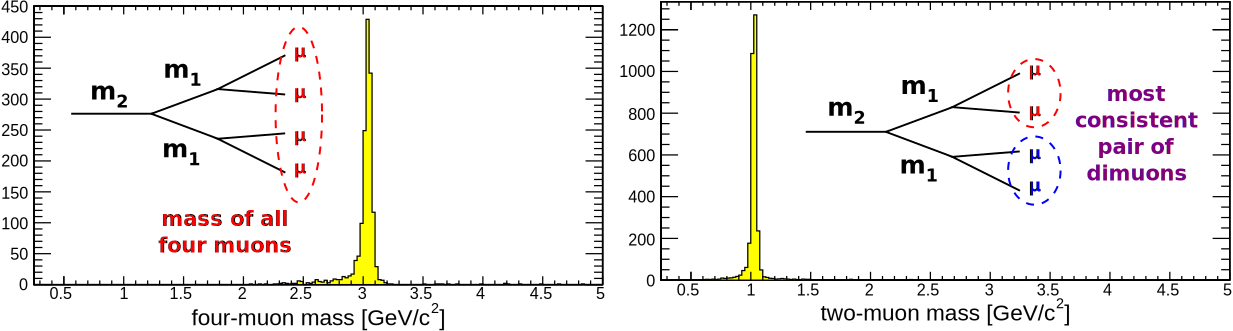
\includegraphics[width=\linewidth]{PLOTS/four-two-muon-mass}

\caption{Identification of fundamental dimuons in a mu-jet containing
  four muons from $m_2 \to m_1 m_1 \to 4\mu$.  The invariant mass of
  all four muons is a sharp peak at $m_2$ (3~GeV/$c^2$ in this
  example), and the invariant mass of the most consistent pair of
  dimuons within this mu-jet is a sharp peak at $m_1$ (1~GeV/$c^2$ in
  this example). \label{fig:four-two-muon-mass}}
\end{figure}

\label{sec:signal_channels}
The number of mu-jets and the number of muons in each mu-jet is used
to classify different signal topologies (any ungrouped muons are
ignored).  A separate mass-peak fit is performed in the
$N$-dimensional fundamental dimuon spectrum of each signal topology,
where $N$ is the number of fundamental dimuons per event.  These
topologies are:
\begin{enumerate}\renewcommand{\labelenumi}{(\alph{enumi})}
\item only one mu-jet per event:
\begin{enumerate}\renewcommand{\labelenumii}{(a-\arabic{enumii})}
\item two muons in the mu-jet with vector-sum $p_T > 80$~GeV/$c$,
  targeting models with a single high-momentum $m_1 \to \mu\mu$,
\item four muons in the mu-jet, targeting models with a low-mass $m_2$
  decaying via $m_2 \to m_1 m_1 \to 4\mu$,
\item more than four muons in the mu-jet, for more complex
  models;
\end{enumerate}

\item two mu-jets per event:
\begin{enumerate}\renewcommand{\labelenumii}{(b-\arabic{enumii})}
\item each mu-jet contains exactly two muons, targeting a model with a
  heavy particle $M$ decaying to two light particles $m_1$: $M \to m_1
  m_1 \to 4\mu$ (this is the NMSSM signature),
\item one mu-jet contains two muons, the other contains four,
  targeting $M \to m_1 m_2$ with $m_1 \to \mu\mu$ and $m_2 \to m_1 m_1
  \to 4\mu$,
\item both mu-jets contain four muons for $M \to m_2 m_2$,
\item one mu-jet with more than four muons, for more complex
  models;
\end{enumerate}

\item more than two mu-jets per event, targeting even more complex models.
\end{enumerate}

Mass-peak fits are used to search for a narrow resonance above
background, with the background normalization determined as a free
parameter in the fit.  The signal is modeled as a narrow Crystal Ball
resonance determined by detector resolution and muon final state
radiation, and the background shape is derived from a mass template in
background control samples.  In cases with two or more fundamental
dimuons per event, the signal is constrained to the diagonal in which
the mass of all fundamental dimuons is nearly equal, while the
background is more uniformly distributed through the space
(Fig.~\ref{fig:diagonal}).  If an $m_1$ mass peak is discovered in one
of the topologies with two or more dimuons, then more complex fits
will be performed to see if they belong to a cascade.  A special 3-D
fit to $m_{h_1}$, $m_{a_1}$, and $m_{a_1}$ is performed for the NMSSM
case $h_1 \to a_1 a_1 \to 2\mu, \, 2\mu$.

\begin{figure}
\begin{center}
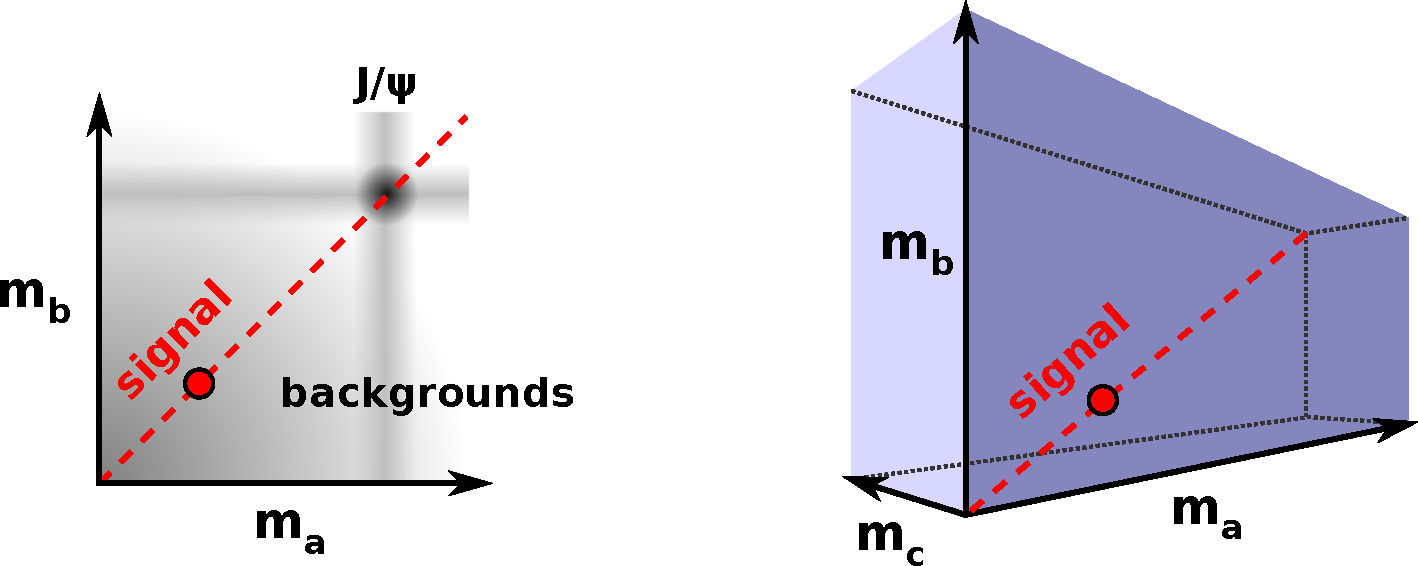
\includegraphics[width=0.75\linewidth]{PLOTS/diagonal.pdf}
\end{center}

\caption{Schematic of multidimensional fits for a single $m_1$ peak
  on Standard Model backgrounds.  The peak must be located on the
  diagonal of the space, while the backgrounds are distributed
  throughout the space. \label{fig:diagonal}}
\end{figure}

\section{Analysis selection and efficiencies}

\subsection{Acceptance}

To avoid introducing complicated model-dependent efficiencies, signal
regions are defined by kinematic cuts that avoid trigger turn-on
curves and regions where the detector loses efficiency for muons that
are very close to one another.  Within the predefined acceptance
regions, the efficiency depends only on muon pseudorapidity $\eta$.
In brief, the acceptance cuts that we use are
\begin{itemize}
\item at least one muon with $p_T > 15$~GeV/$c$ and $|\eta| < 0.9$ per
  event (muon barrel system trigger plateau);
\item all other muons must have $p_T > 5$~GeV/$c$ and $|\eta| < 2.4$
  (offline reconstruction plateau).
\end{itemize}

\fixme{following part unnecessary?}

The cuts on muon kinematics imply the following endpoints in mu-jet kinematics:
\begin{itemize}
\item at least one mu-jet with $p_T > 20$~GeV/$c$ and $|\eta| \lesssim 0.9$ per event;
\item all other mu-jets (if any) with $p_T > 10$~GeV/$c$ and $|\eta| \lesssim 2.4$.
\end{itemize}
The $\eta$ endpoints on mu-jets are only tight in the limit of highly
boosted mu-jets, where the muons to which we applied the selection are
nearly collinear.  The mu-jet momentum minima are indicated with
dashed lines in Fig.~\ref{fig:openingangle_dr}.

The trigger efficiency and offline muon reconstruction efficiency are
derived as simple factors from $Z \to \mu\mu$ data using a
tag-and-probe technique.

\subsection{Reconstruction and efficiency}

Arbitrated TrackerMuons muons.

\subsection{Trigger efficiency}

For all signatures, we select events with the lowest unprescaled,
unisolated, single-muon trigger available (see
Appendix~\ref{sec:motivation_for_trigger_choice} for motivation).  In
the 2010A dataset (May--Aug 2010, 3~pb$^{-1}$), this is HLT\_Mu9 and
in the 2010B dataset (Sep--Oct 2010, 32~pb$^{-1}$), this is HLT\_Mu15.
Since the HLT\_Mu15 trigger does not exist in the 2010A data, we
simulate it by requiring an L3 muon reconstructed with $p_T >
15$~GeV/$c$.  We also require at least one $p_T > 15$~GeV/$c$, $|\eta|
< 0.9$ muon offline, to be insensitive to the shape of trigger turn-on
curves and nearby-muon inefficiencies in the endcap.  The $p_T$
resolution of L3 and offline muons are both dominated by tracker
resolution.

The trigger response was studied in a generic way by simulating muon
pairs with uniform mass, pair $p_T$, and pair $\eta$ distributions
(dimuon-gun MC).  It is important to isolate dependencies of the
efficiency on all physical variables in this unrealistic sample, as
such a dependence would lead to model-dependent inefficiency in
realisic cases.

In a dimuon-gun subsample with at least one $p_T > 15$~GeV/$c$ muon,
the HLT\_Mu15 efficiency versus dimuon mass, $\eta$, and $p_T$ are
shown in Fig.~\ref{fig:triggersimulation}.  \fixme{Need to change all
  Mu11 plots to Mu15.}  The endcap region is inefficient for low-mass
dimuons, and this inefficiency has a slight dependence on pair $p_T$.

To diagnose this further, we plot the efficiency as a function of how
close the muon trajectories approach each other in the muon system
(Fig.~\ref{fig:triggersimulation2}).  The closeness of the muon
trajectories is quantifed for $0.9 < |\eta| < 2.1$ on a plane at $|z|
= 700$~cm (ME1/2), in terms of separation in azimuthal position
$\Delta \phi = \phi_{\mu^+} - \phi_{\mu^-}$ and and radial position
$\Delta r = r_{\mu^+} - r_{\mu^-}$: the efficiency drops
by a factor of two when $|\Delta \phi| < 0.2$ and $|\Delta r/z| <
0.2$, though this efficiency loss is independent of leading muon
$p_T$, as evidenced by the turn-on curve within the spot.  Dimuons of
different mass/momentum combinations sample this spot differently, as
indicated by the labeled contour lines.  Since the masses and momentum
distributions of new physics dimuons is unknown, the endcap trigger
efficiency cannot be quantified.  That is why we require at least one
above-threshold muon in the barrel per event.  (This study was
performed with a 2010B-like endcap trigger simulation--- no ME1/1
singles and modified ghost suppression--- though the conclusion is the
same for the 2010A-like endcap trigger simulation.)

\begin{figure}[p]
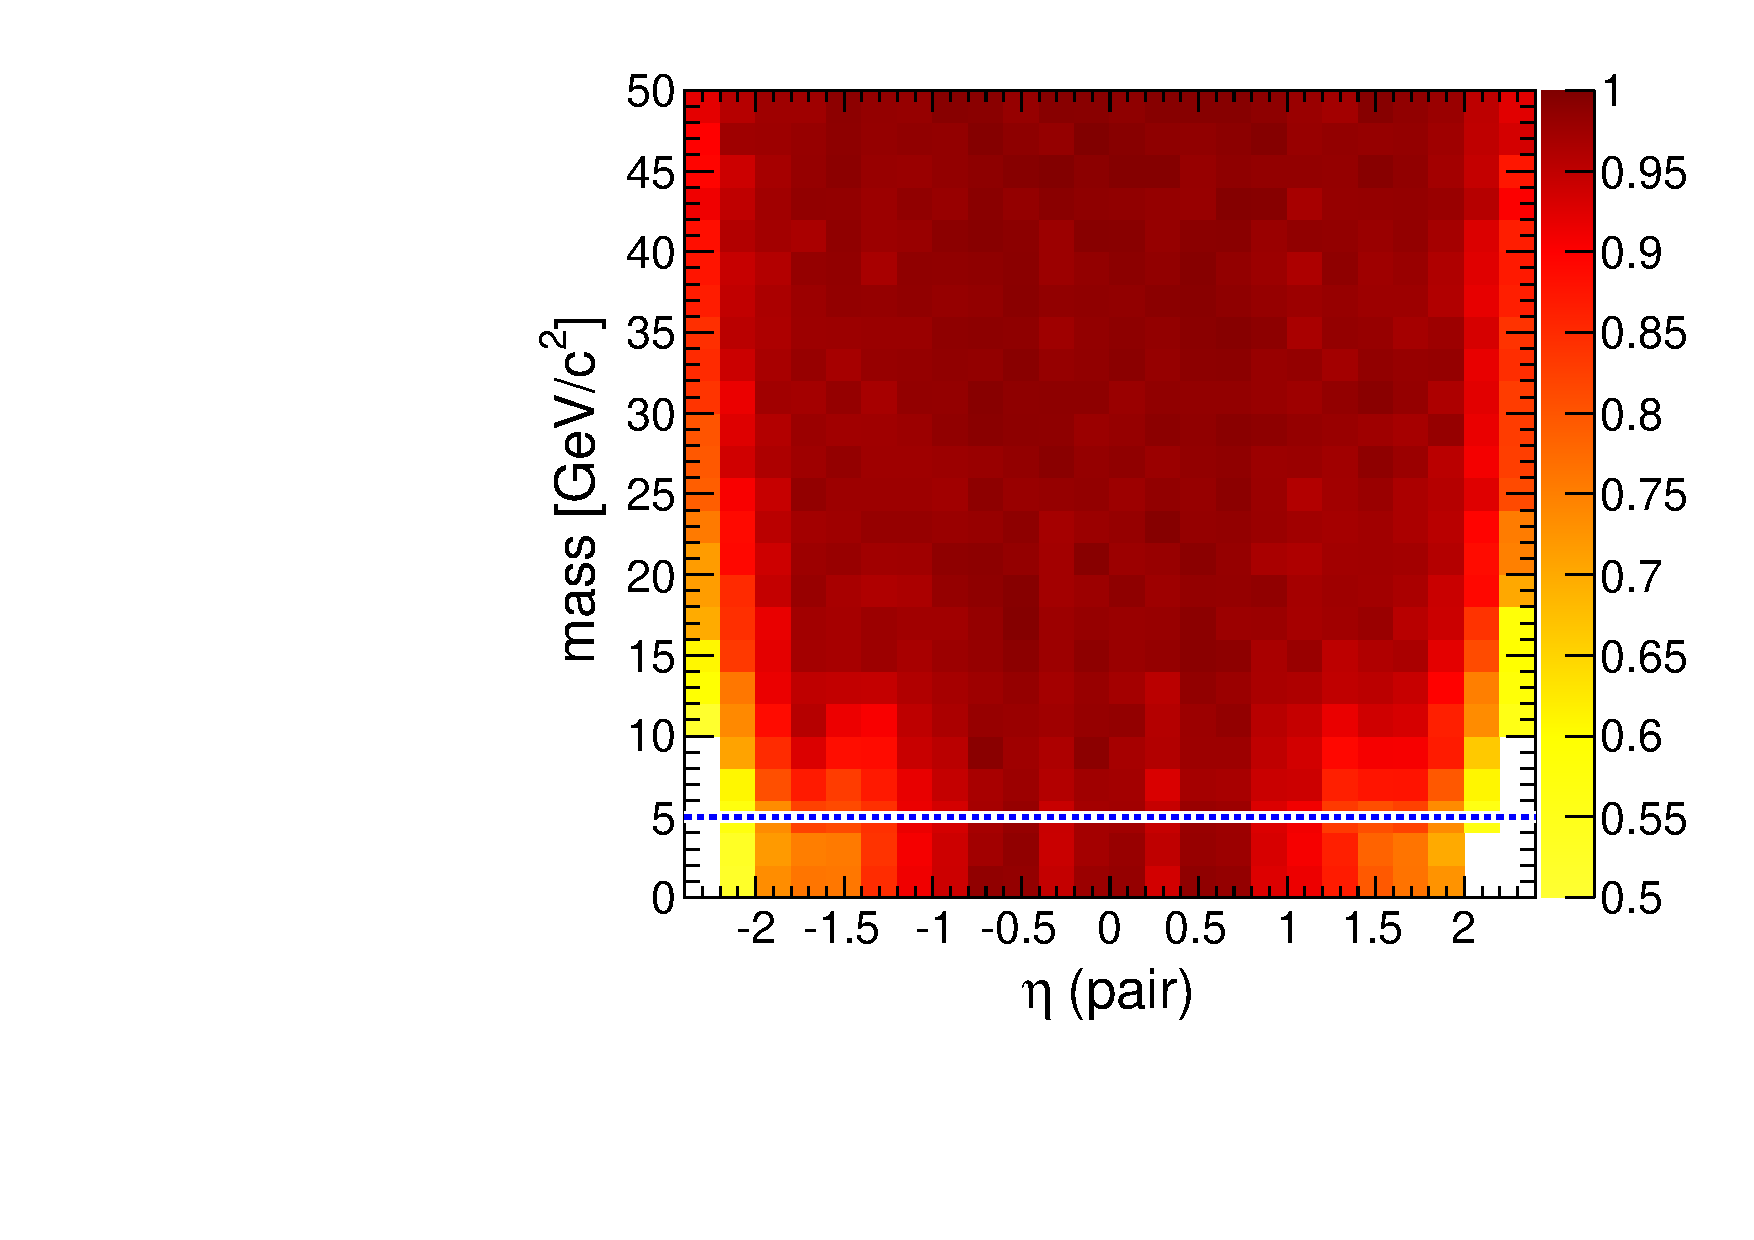
\includegraphics[width=0.48\linewidth]{PLOTS/masseta_pluscut_Mu11.pdf} \hfill
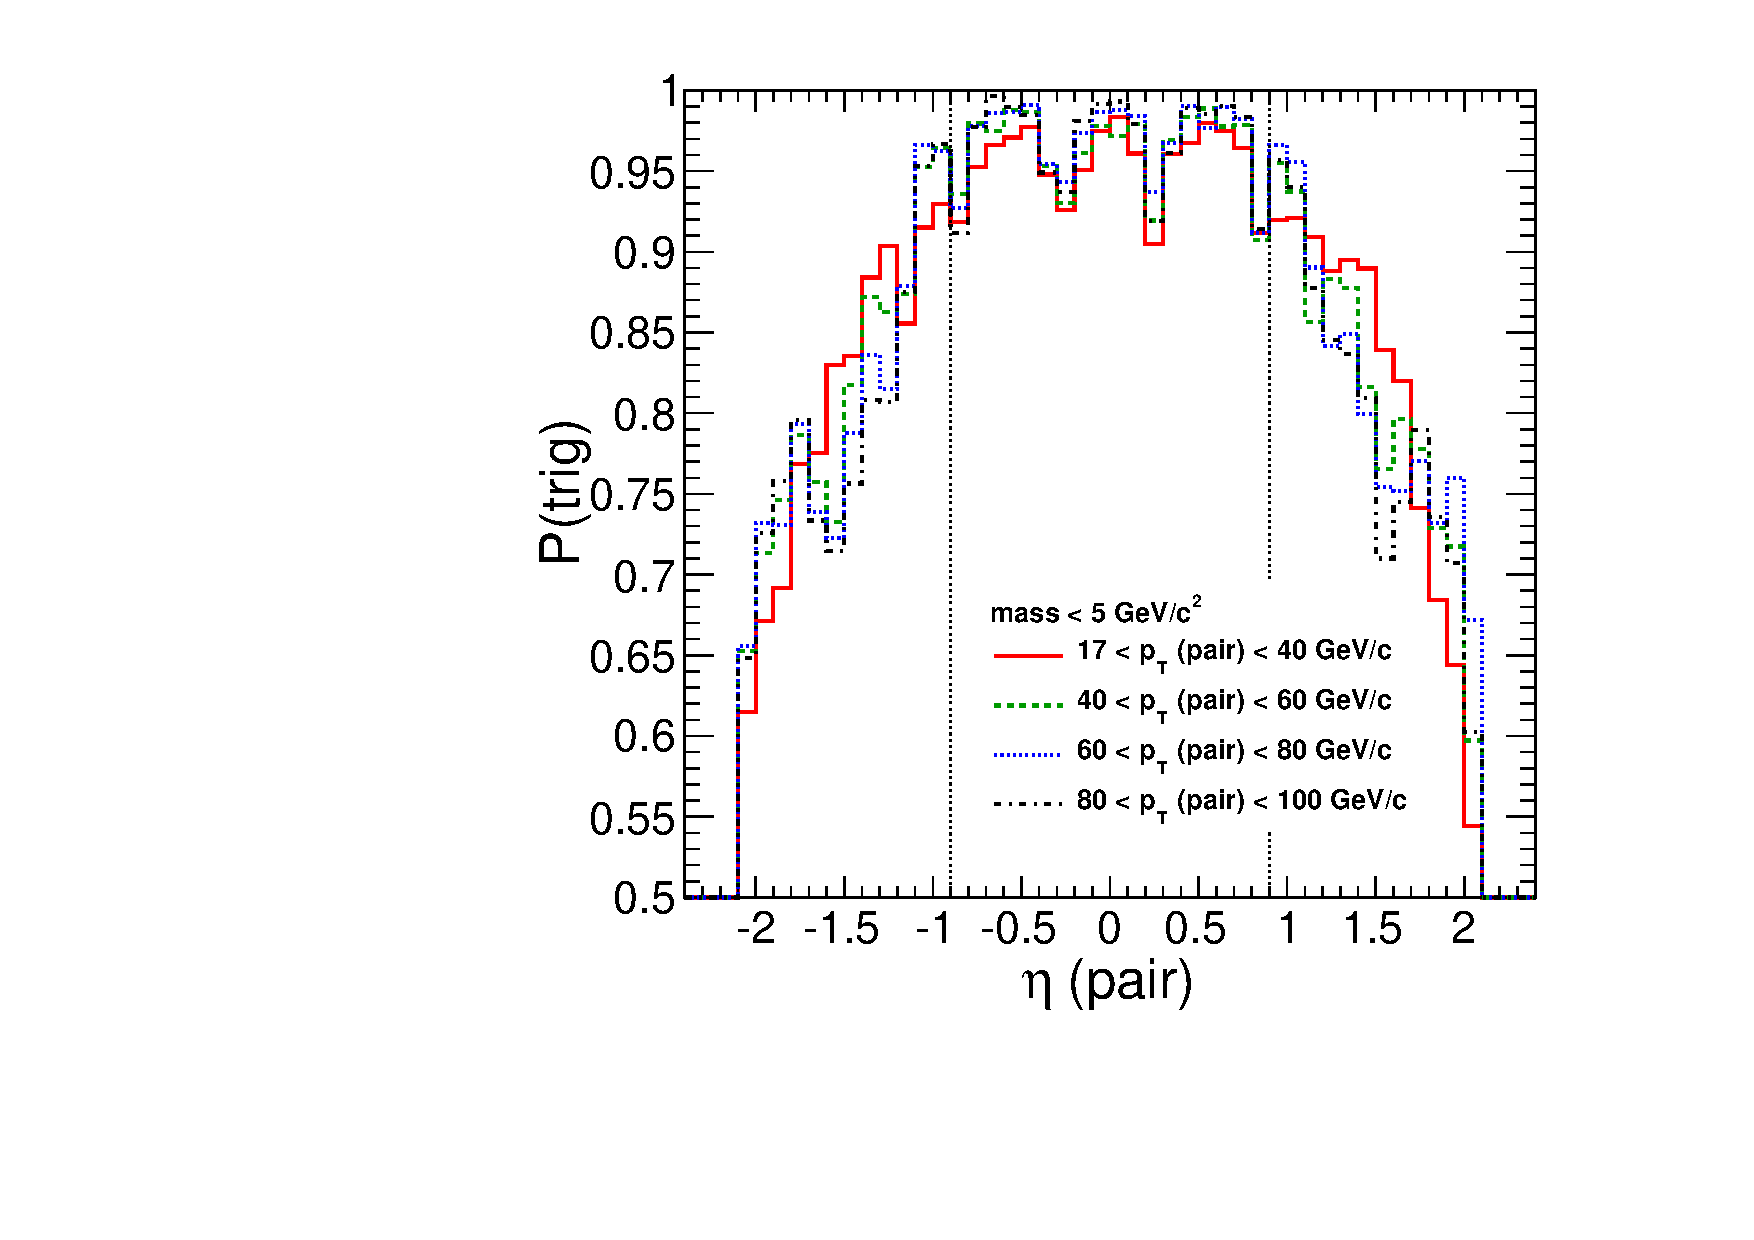
\includegraphics[width=0.48\linewidth]{PLOTS/eta_mass5cut_pluscut_Mu11_alt.pdf}

\caption{HLT\_Mu11 trigger efficiency as a function of mass, momentum,
  and pseudorapidity of dimuons in a dimuon-gun simulation.  In both
  plots, trigger efficiency is the fraction of event passing the
  trigger in a sample with at least one $p_T > 15$~GeV/$c$ muon, the
  other unconstrained.  \label{fig:triggersimulation}}
\end{figure}

\begin{figure}[p]
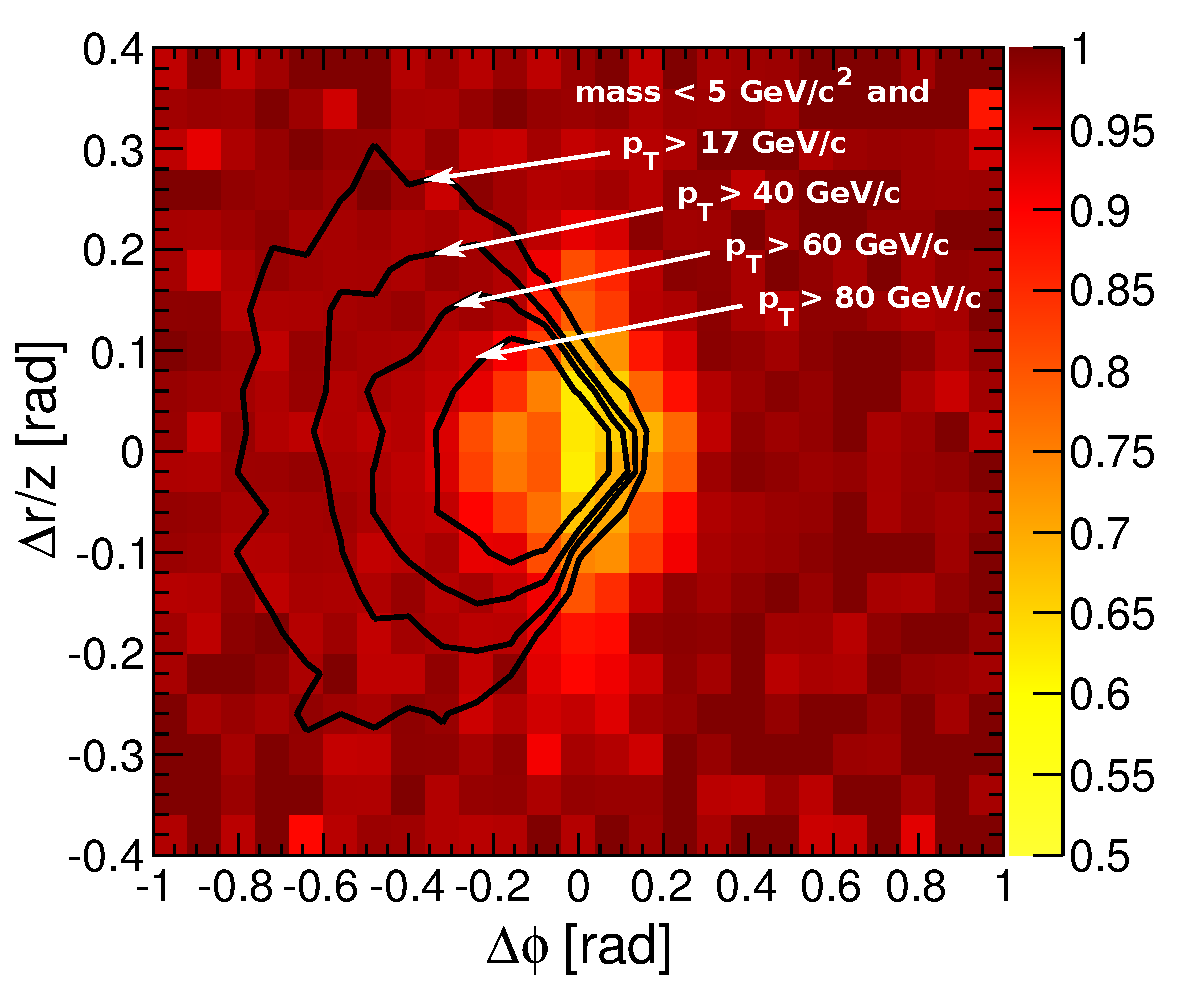
\includegraphics[width=0.48\linewidth]{PLOTS/endcap_dphidr_HLTMu11_09_21.pdf} \hfill
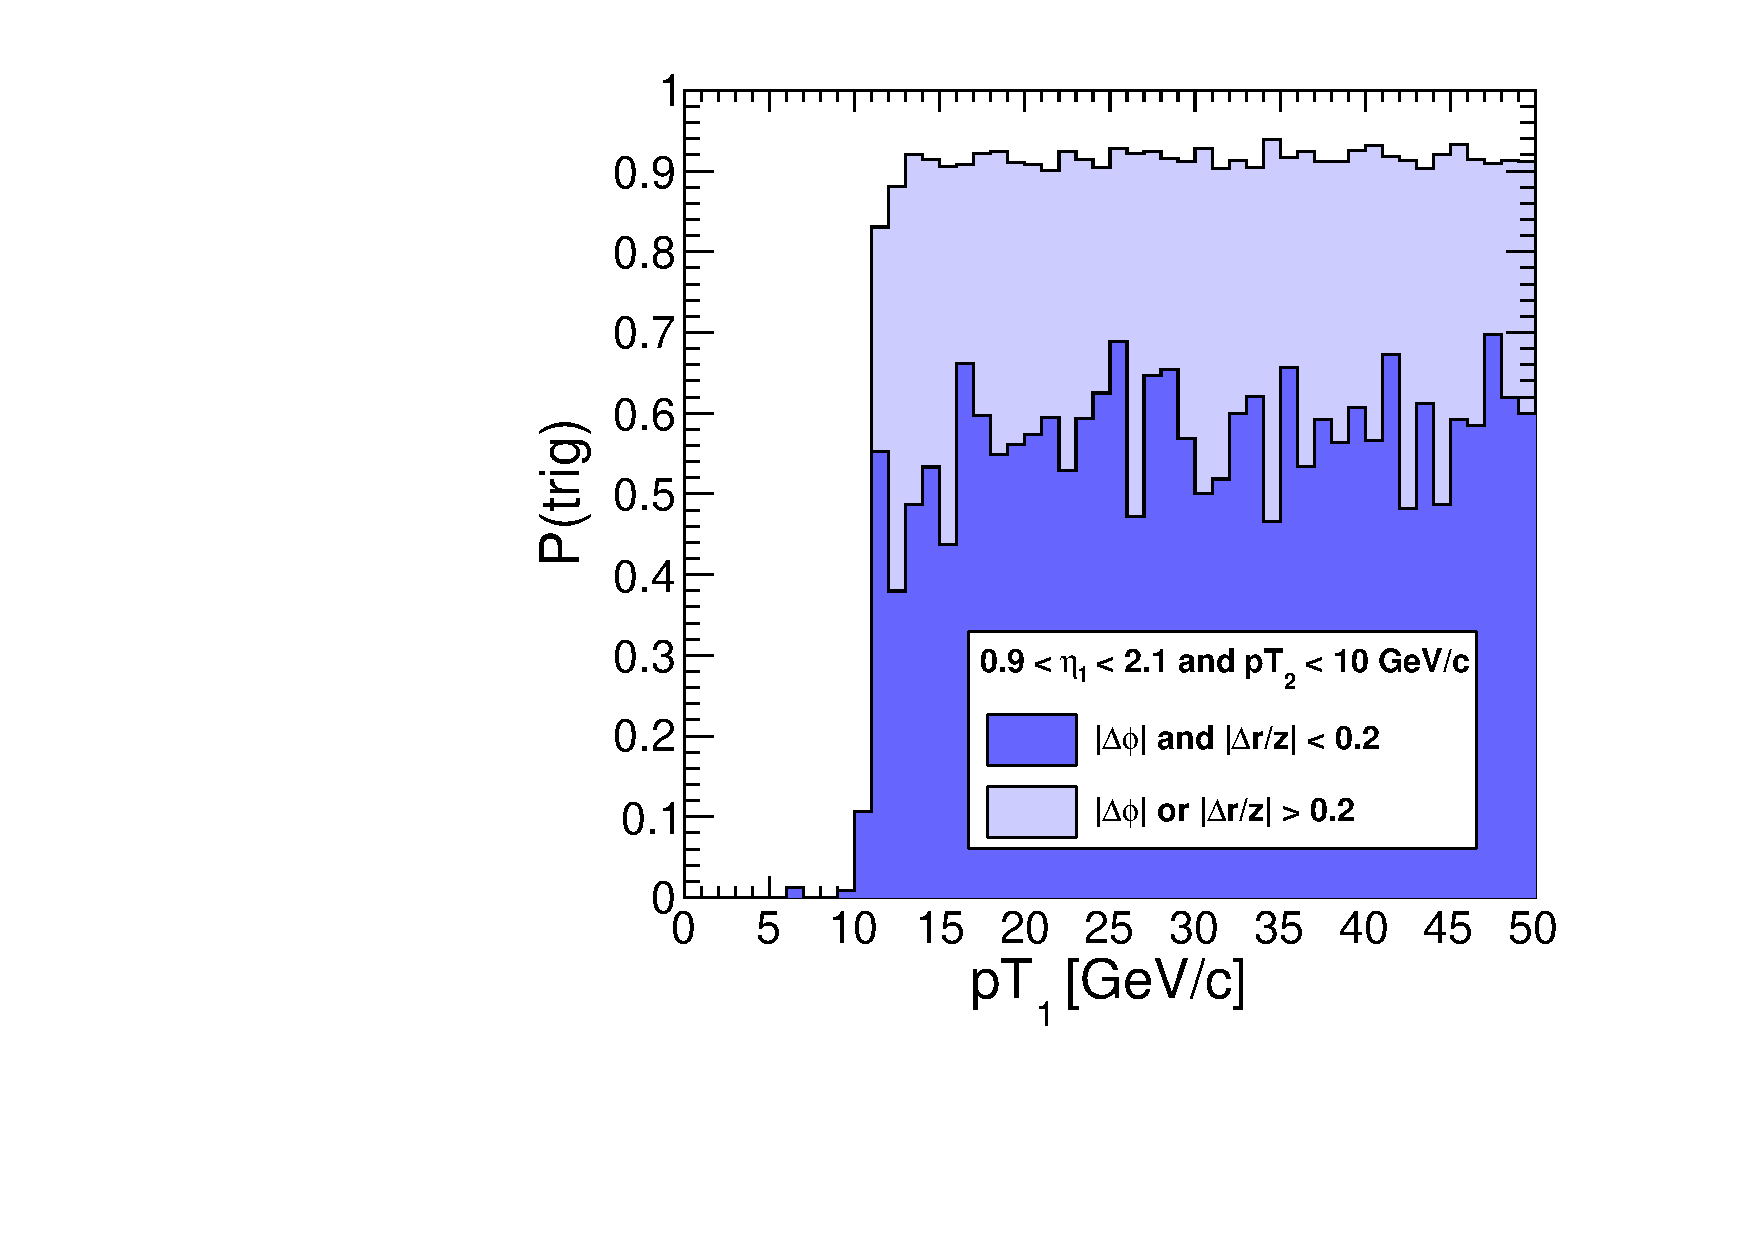
\includegraphics[width=0.48\linewidth]{PLOTS/trigger_turnonMu11.pdf}

\caption{Diagnostic of HLT\_Mu11 $p_T$ dependence in $0.9 < |\eta| <
  2.1$.  Left: trigger efficiency (color scale) with one $p_T >
  15$~GeV/$c$ muon, the other unconstrained, as a function of
  separation of muons in the muon system.  Different mass/momentum
  combinations (the labeled contour lines) sample this spot to
  differing degrees.  The trigger turn-on curve in the spot is
  unaffected; it is the plateau efficiency that is
  lowered. \label{fig:triggersimulation2}}
\end{figure}

\fixme{Need to update all HLT\_Mu11 plots to HLT\_Mu15 and simplify
  the presentation of this.  In the exotica talk, we have a
  side-by-side comparison of efficiency vs.\ $\eta$ for overlapping
  and non-overlapping trajectories: the difference is dramatic.}

\subsection{Measurement of efficiency within acceptance cuts}

\fixme{Reconstruction and trigger efficiency from $Z$ tag-and-probe}

\section{Signal mass spectrum shape}
\label{sec:signal_mass_spectrum_shape}

Resonances coupling weakly to the Standard Model are by definition
narrow, so their lineshapes are dominated by detector resolution and
final state radiation of a photon from one of the muons.  The Standard
Model provides four resonances in our mass range of interest,
$\omega$, $\phi$, $J/\psi$, and $\psi'$, which we use to calibrate the
signal lineshapes.  These resonances are typically produced with low
momentum, so we additionally simulate low and high momentum resonances
with a dimuon-gun Monte Carlo.

The most general lineshape used in this study is a first-order Crystal
Ball double-Gaussian with a linear background.  None of the resolution
studies use all of the features of this curve in a single fit, but
each feature is used in some study.  An expression for the curve as
$f(m)$ with $m$ as invariant mass (in GeV/$c^2$) is
\begin{multline}
S(m; m_0, \sigma, \alpha, f_{0.07}, p_0, p_1) = \\ p \bigg[ (1 -
  f_{0.07}) \, CB(m; m_0, \sigma, \alpha) + f_{0.07}
  \, G_{0.07}(m; m_0) + p_0 + p_1 m \bigg]
\end{multline}
where
\begin{equation}
CB(m; m_0, \sigma, \alpha) = \left\{ \begin{array}{c l} \dfrac{1}{\sqrt{2\pi}\, \sigma} \exp\left(-(m - m_0)^2 / (2 \sigma^2)\right) & \mbox{if $(m - m_0)/\sigma > -\alpha$} \\
\dfrac{2}{5 \sigma} \exp\left(-\alpha^2/2\right)/(1 - \alpha^2 - (m-m_0)/\sigma) & \mbox{otherwise} \end{array} \right.
\end{equation}
and
\begin{equation}
G_{0.07}(m; m_0) = \frac{1}{\sqrt{2\pi}\, 0.07} \exp\left(-(m - m_0)^2 / (2 \cdot 0.07^2)\right) + p_0 + p_1 m \bigg]\mbox{.}
\end{equation}
The peak of the mass distribution (true mass of the particle in this
parameterization) is $m_0$ (GeV/$c^2$), with core resolution $\sigma$
(GeV/$c^2$).  The Crystal Ball parameter $\alpha$ indicates where the
core Gaussian smoothly connects to a low-side $1/(m-m_0)$ tail (in
number of standard deviations below the peak).  A second,
0.07~GeV/$c^2$ wide Gaussian is scaled by $f_{0.07}$; for most
observed distributions, $f_{0.07} \to 0$.  The linear background is
$p_0 + p_1 m$.

Fits to the Standard Model resonances are shown in
Fig.~\ref{fig:respeak_fits}.  The data are required to contain
exactly two muons with vector-sum $p_T < 80$~GeV/$c$, where at least
one has $p_T > 15$~GeV/$c$ and $|\eta| < 0.9$.  The masses are all
fixed to PDG values.  In the $\omega$ fit, the $\rho$ is included
with an intrinsic width fixed to its PDG value and allowed to float in
normalization, as an additional background.  In all resonance-fits,
the double-Gaussian was suppressed ($f_{0.07}$ fixed at zero), since
the double-Gaussian behavior is observed only in the endcap.  Only in
the $J/\psi$ fit is the Crystal Ball tail allowed to float: the fitted
value, $\alpha = 2.04 \pm 0.11$, is fixed in the other three resonance
fits.  \fixme{Should say something about the poor $J/\psi$ fit or make
it better, not that it matters for the analysis.}

\begin{figure}
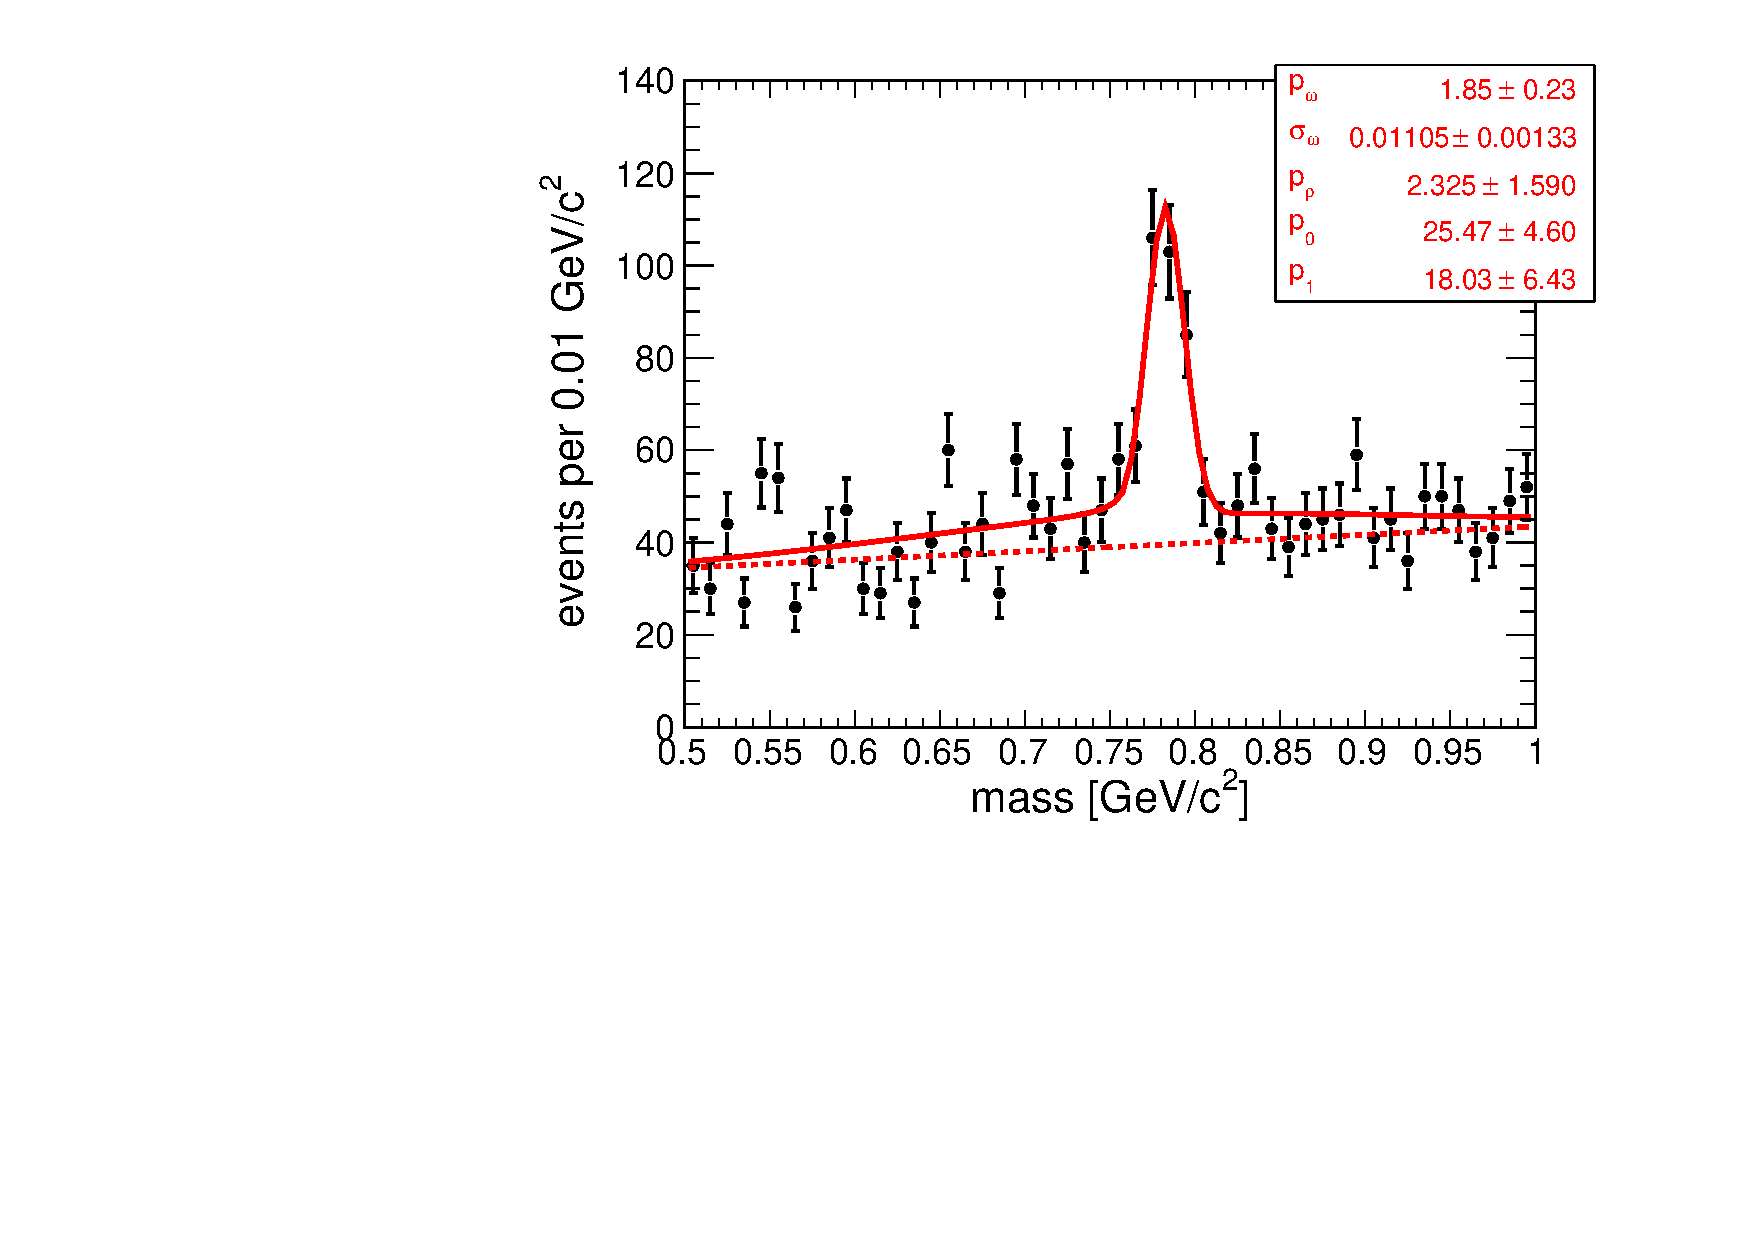
\includegraphics[width=0.5\linewidth]{PLOTS/respeak_omega.pdf} \hfill
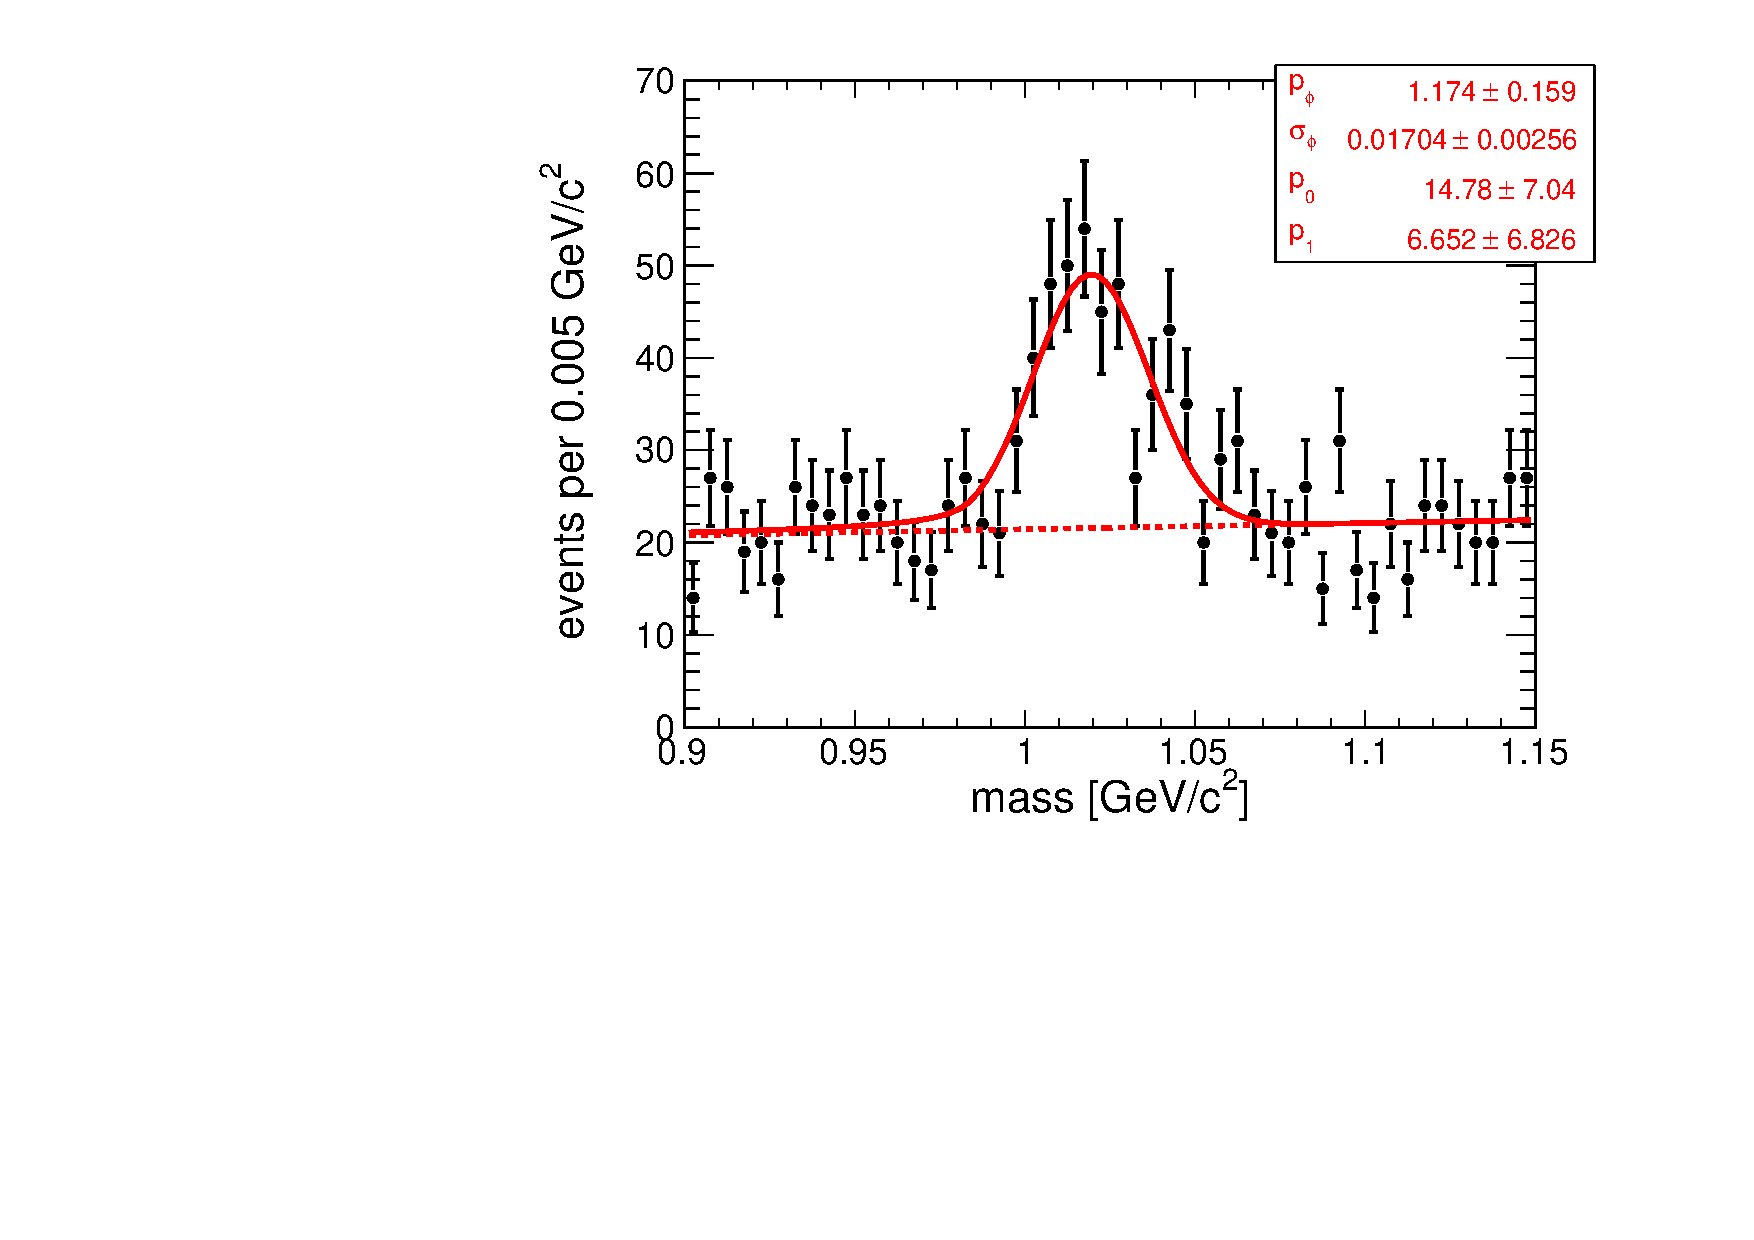
\includegraphics[width=0.5\linewidth]{PLOTS/respeak_phi.pdf}

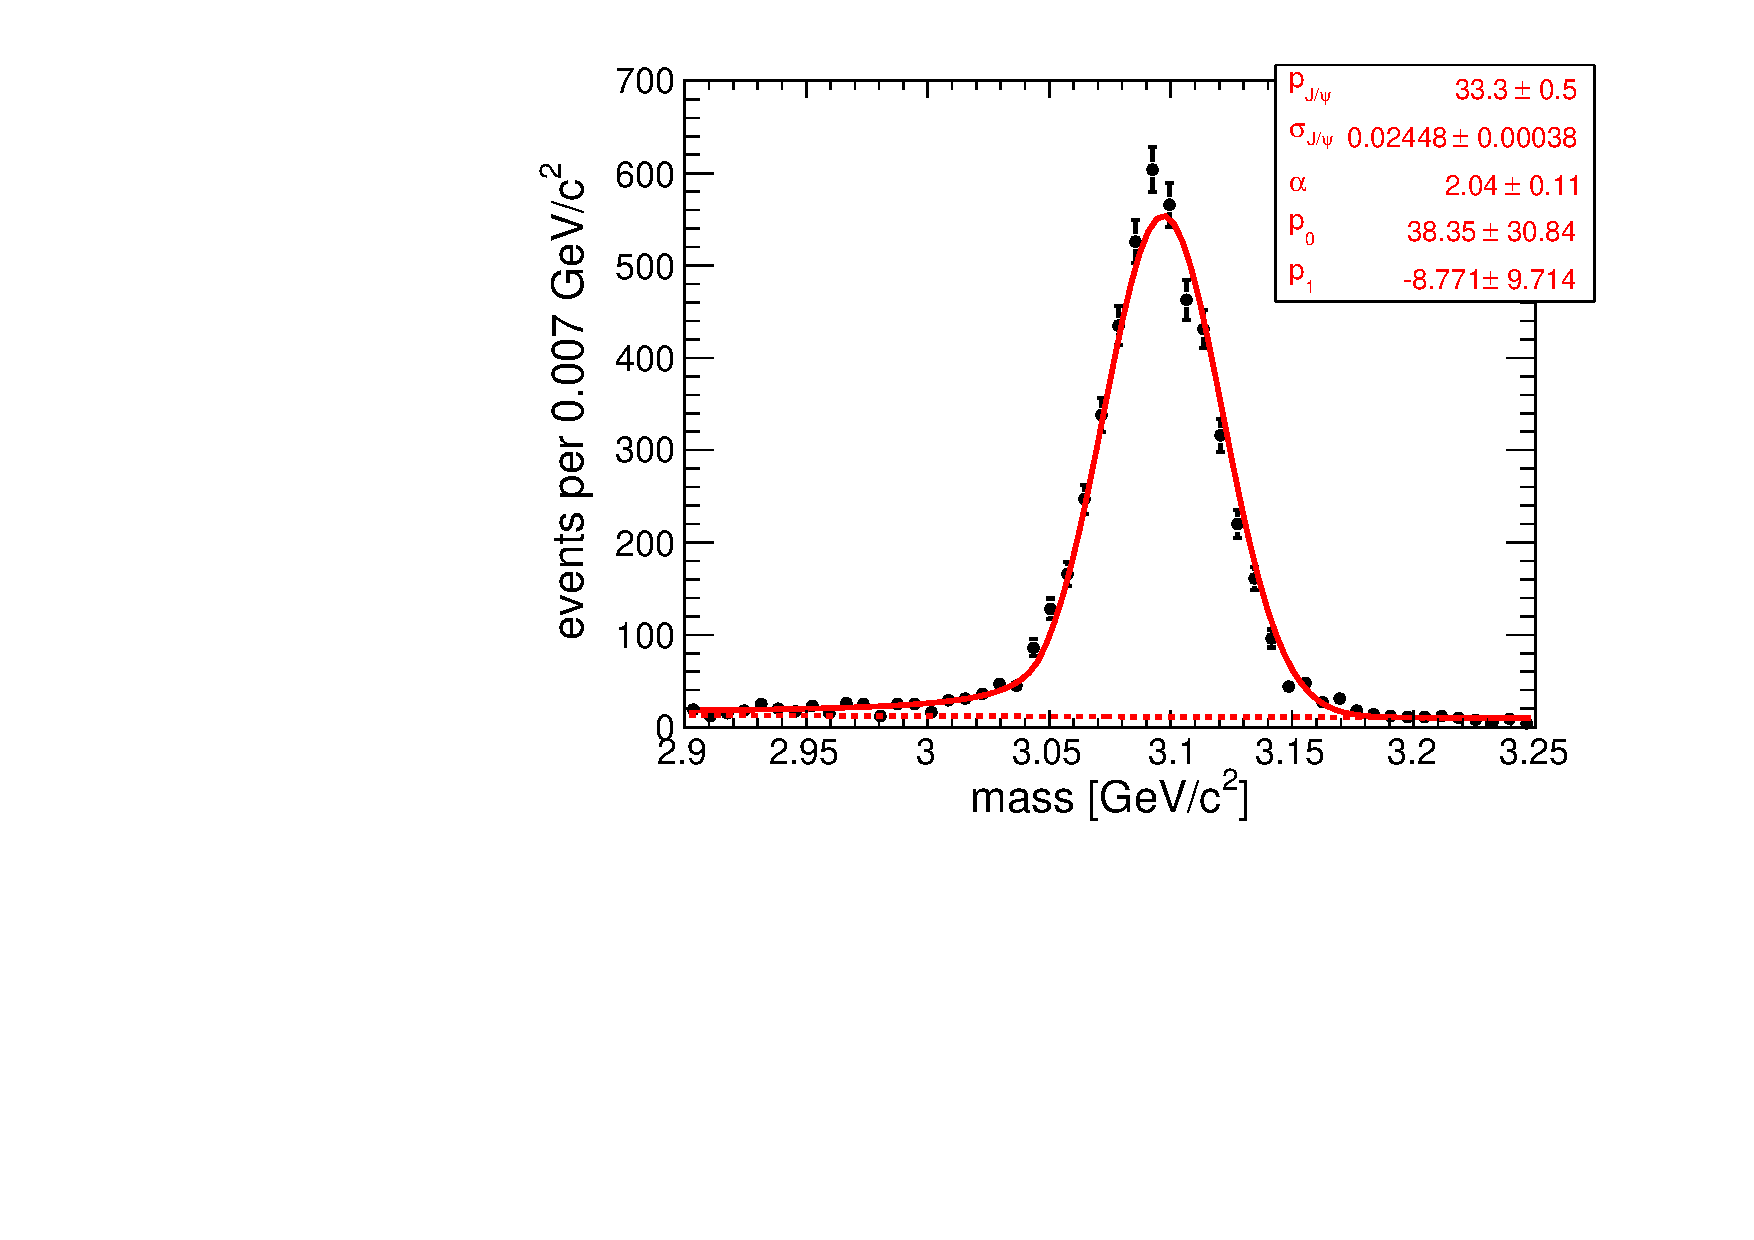
\includegraphics[width=0.5\linewidth]{PLOTS/respeak_jpsi.pdf} \hfill
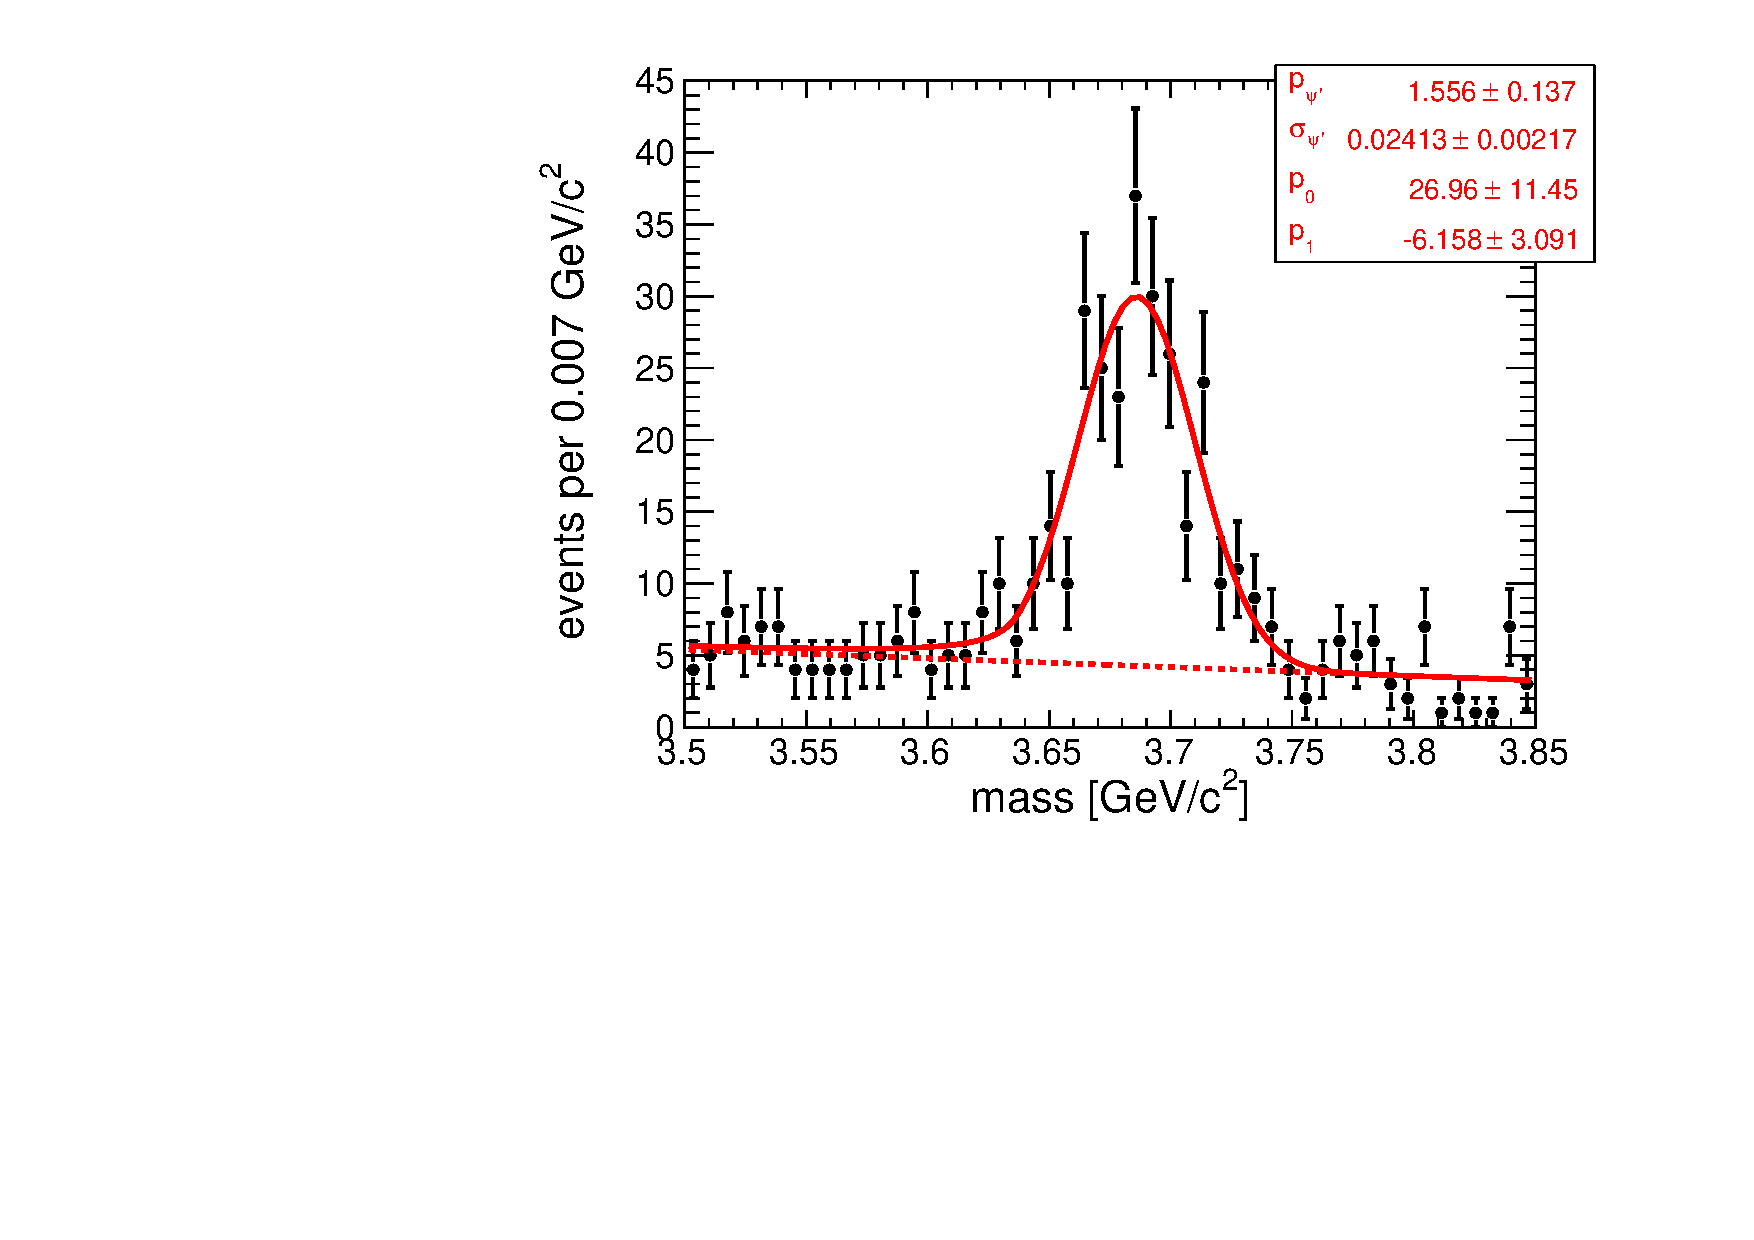
\includegraphics[width=0.5\linewidth]{PLOTS/respeak_psiprime.pdf}

\caption{Four resonance mass peak fits in dimuon data: $\omega$
  (top-left), $\phi$ (top-right), $J/\psi$ (bottom-left), and $\psi'$
  (bottom-right).  All masses are fixed to PDG values; see text for a
  complete list of fixed/free parameters. \label{fig:respeak_fits}}
\end{figure}

To quantify the resolution of dimuons over the whole $\eta$ range, we
used a dataset with three muons: two belong to the same mu-jet and the
third is used to satisfy the trigger ($p_T > 15$~GeV/$c$, $|\eta| <
09$, matched to a trigger-level muon).  Since these events are much
more rare than dimuons, we only fit the $J/\psi$, and fix $\alpha$ to
the value quoted above and $f_{0.07}$ to zero.  The fitted peak is
presented in Fig.~\ref{fig:respeak_jpsi2}.

\begin{figure}
\begin{center}
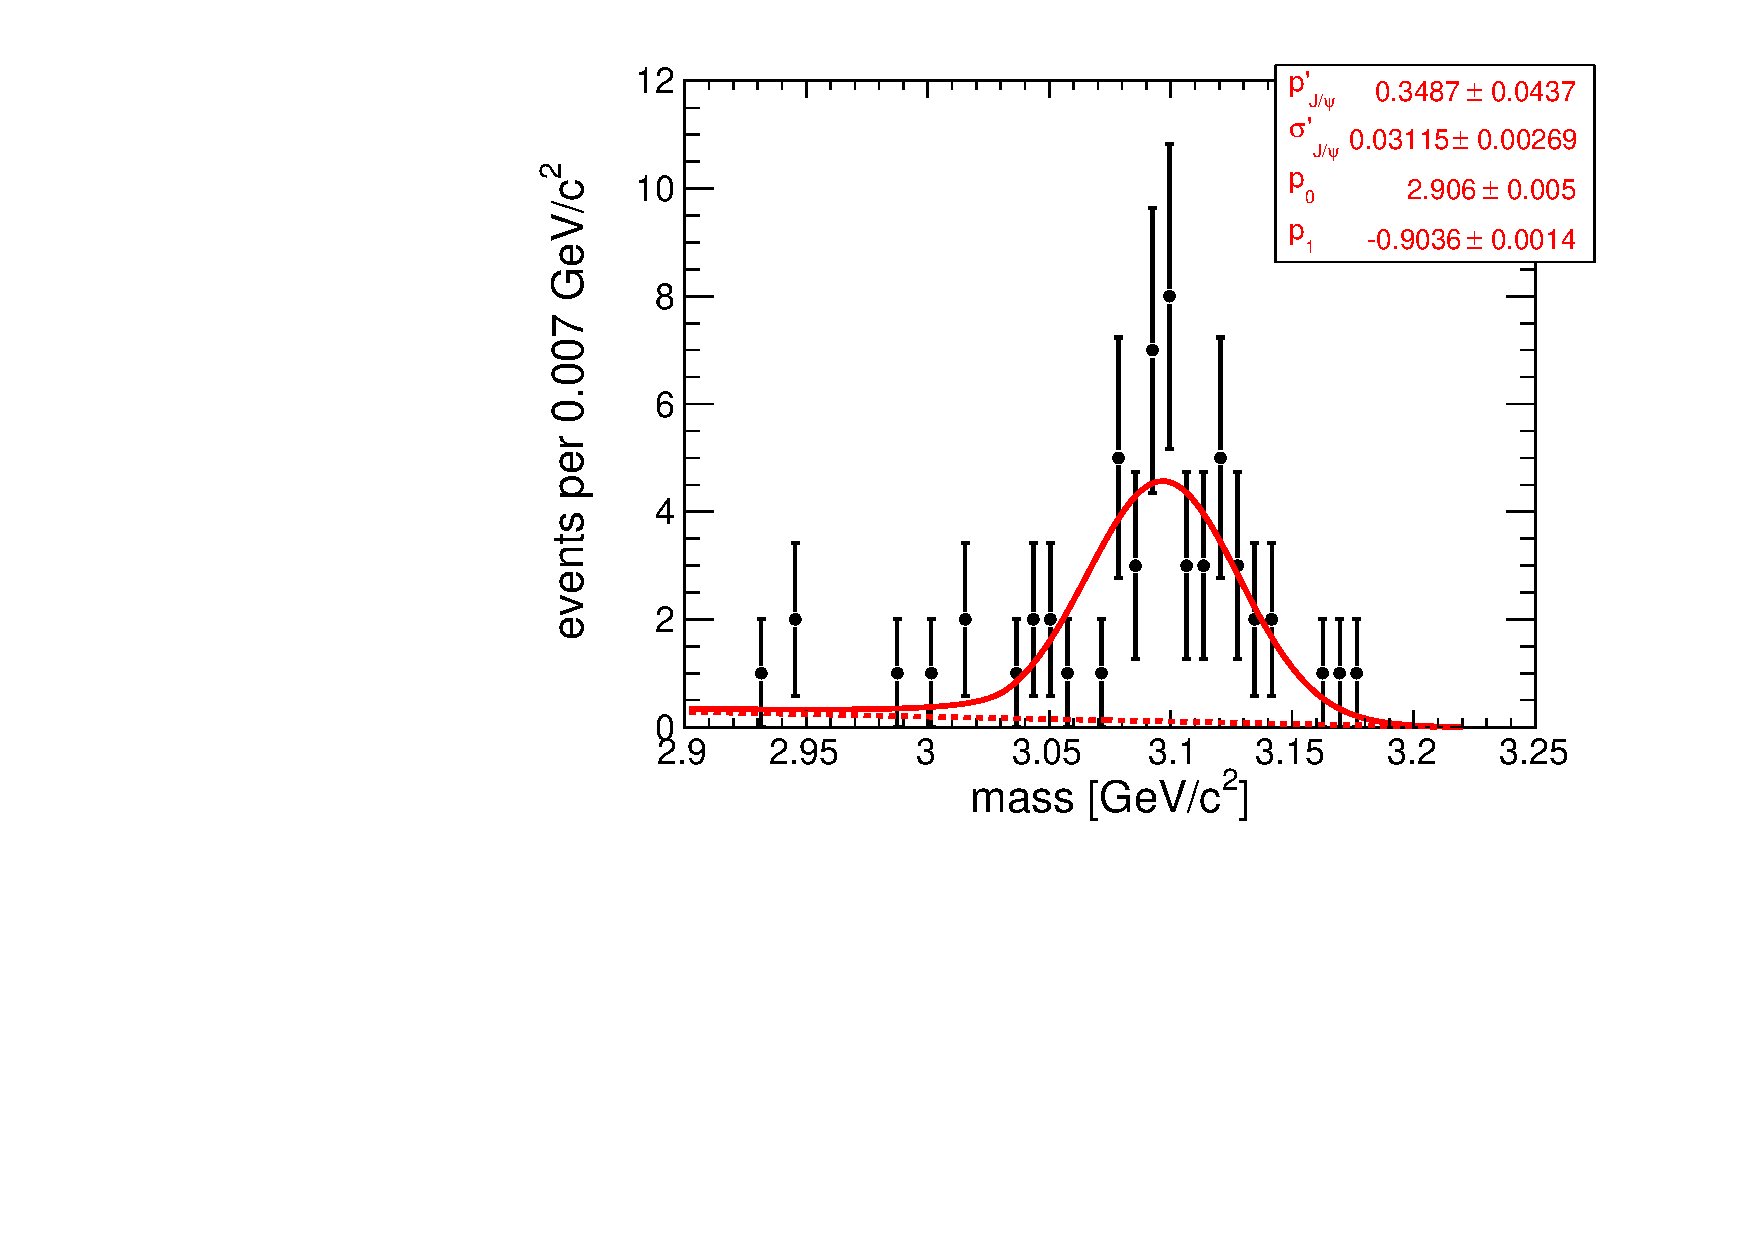
\includegraphics[width=0.5\linewidth]{PLOTS/respeak_jpsi2.pdf}
\end{center}

\caption{$J/\psi$ fit in dimuon-plus-muon data, where the third muon
  is used to satisfy the trigger.  The $\sigma$ observed in this fit
  applies to the full $\eta$ range, not just the
  barrel. \label{fig:respeak_jpsi2}}
\end{figure}

For more sensitivity to extremes in $p_T$ and $\eta$, distributions of
reconstructed mass minus generator-level mass from the dimuon gun
Monte Carlo were fitted to double Gaussians.  Backgrounds ($p_0$ and
$p_1$) and final-state radiation ($\alpha$) were not included in the
fit because the effects were not simulated.
Figure~\ref{fig:resolution} summarizes the results of these fits in
bins of dimuon $p_T$, mass, and $\eta$ coverage.  The results of the
resonance data fits are overlaid for comparison.  The core Gaussian
dependence on $p_T$ and $\eta$ are weak, but higher momenta and larger
$\eta$ coverage yield slightly wider core resolutions.  The
double-Gaussian part of the distribution, however, grows strongly as a
function of mass for high-$p_T$ dimuons in the endcap.

\begin{figure}
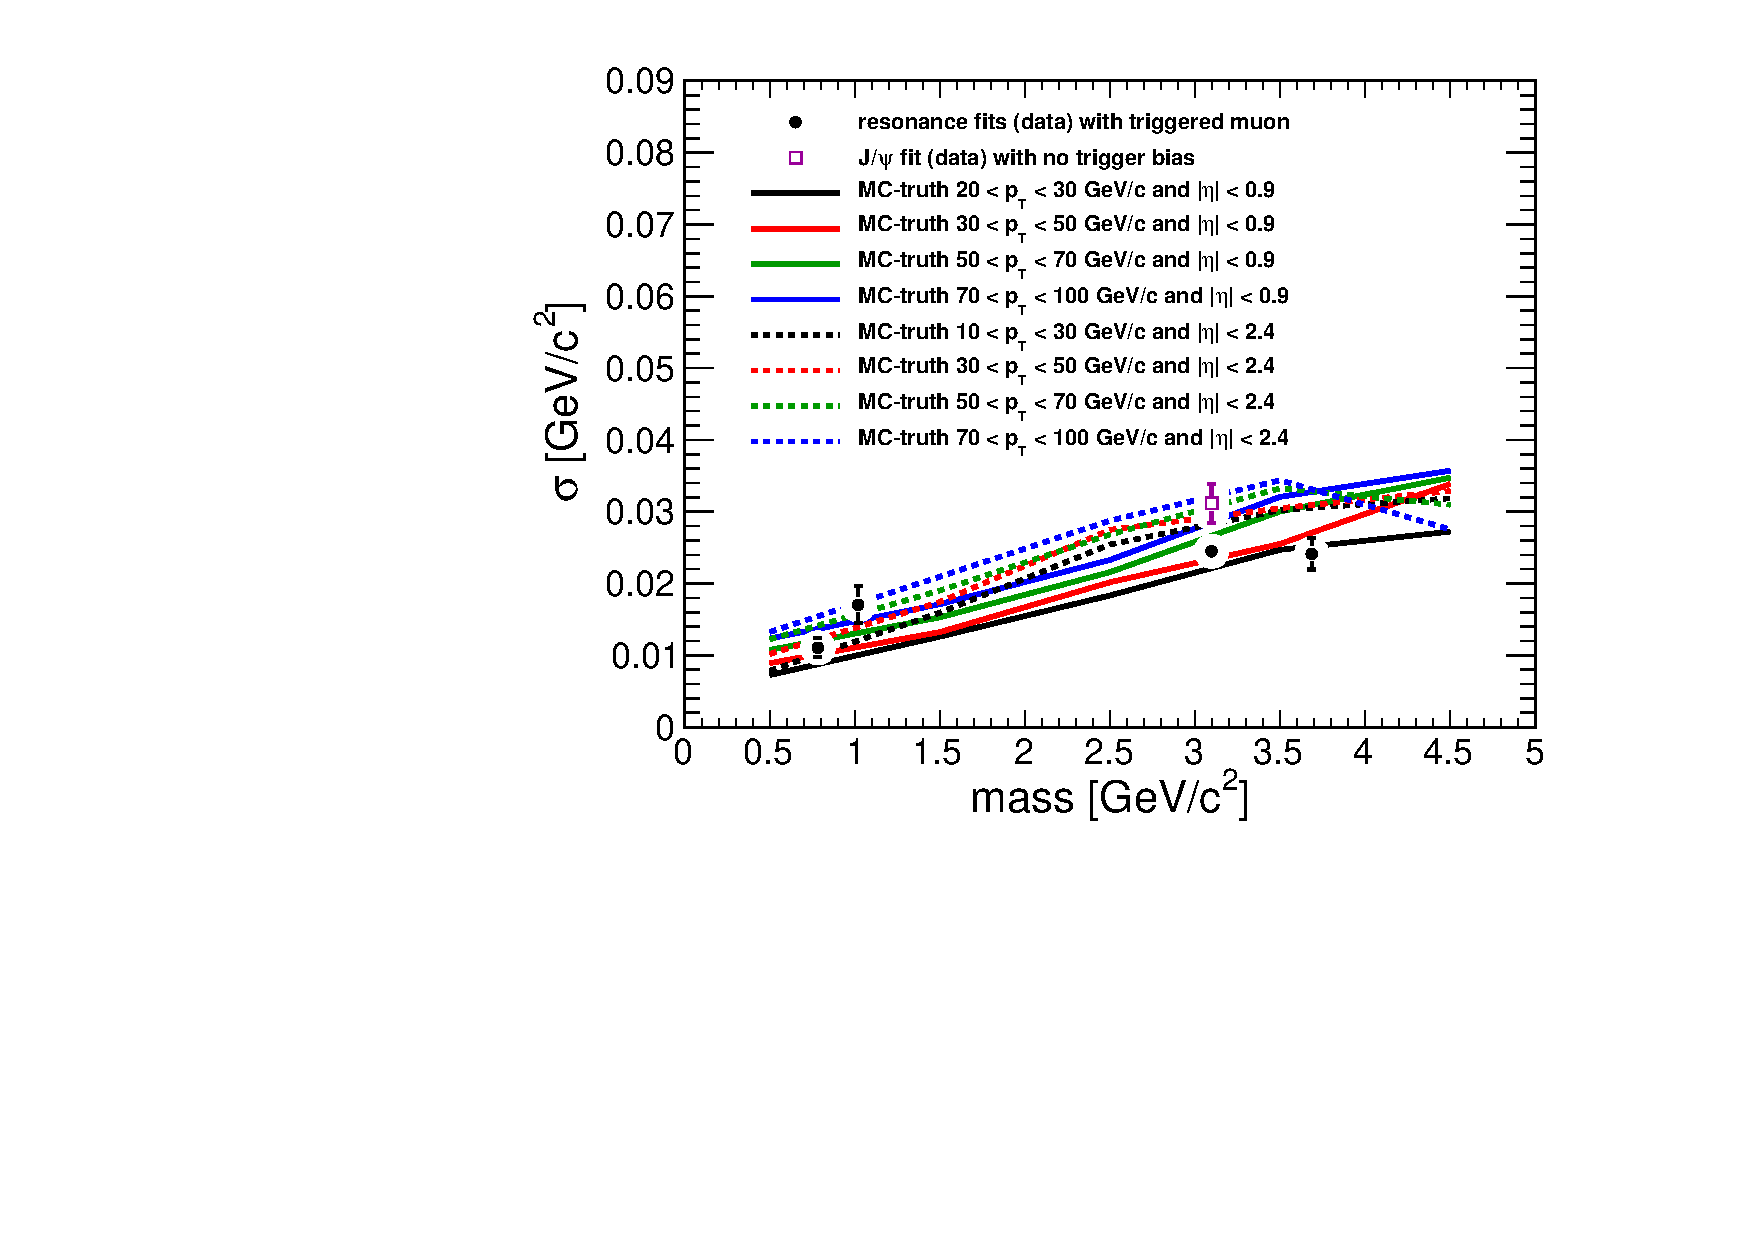
\includegraphics[width=0.5\linewidth]{PLOTS/resolution.pdf}
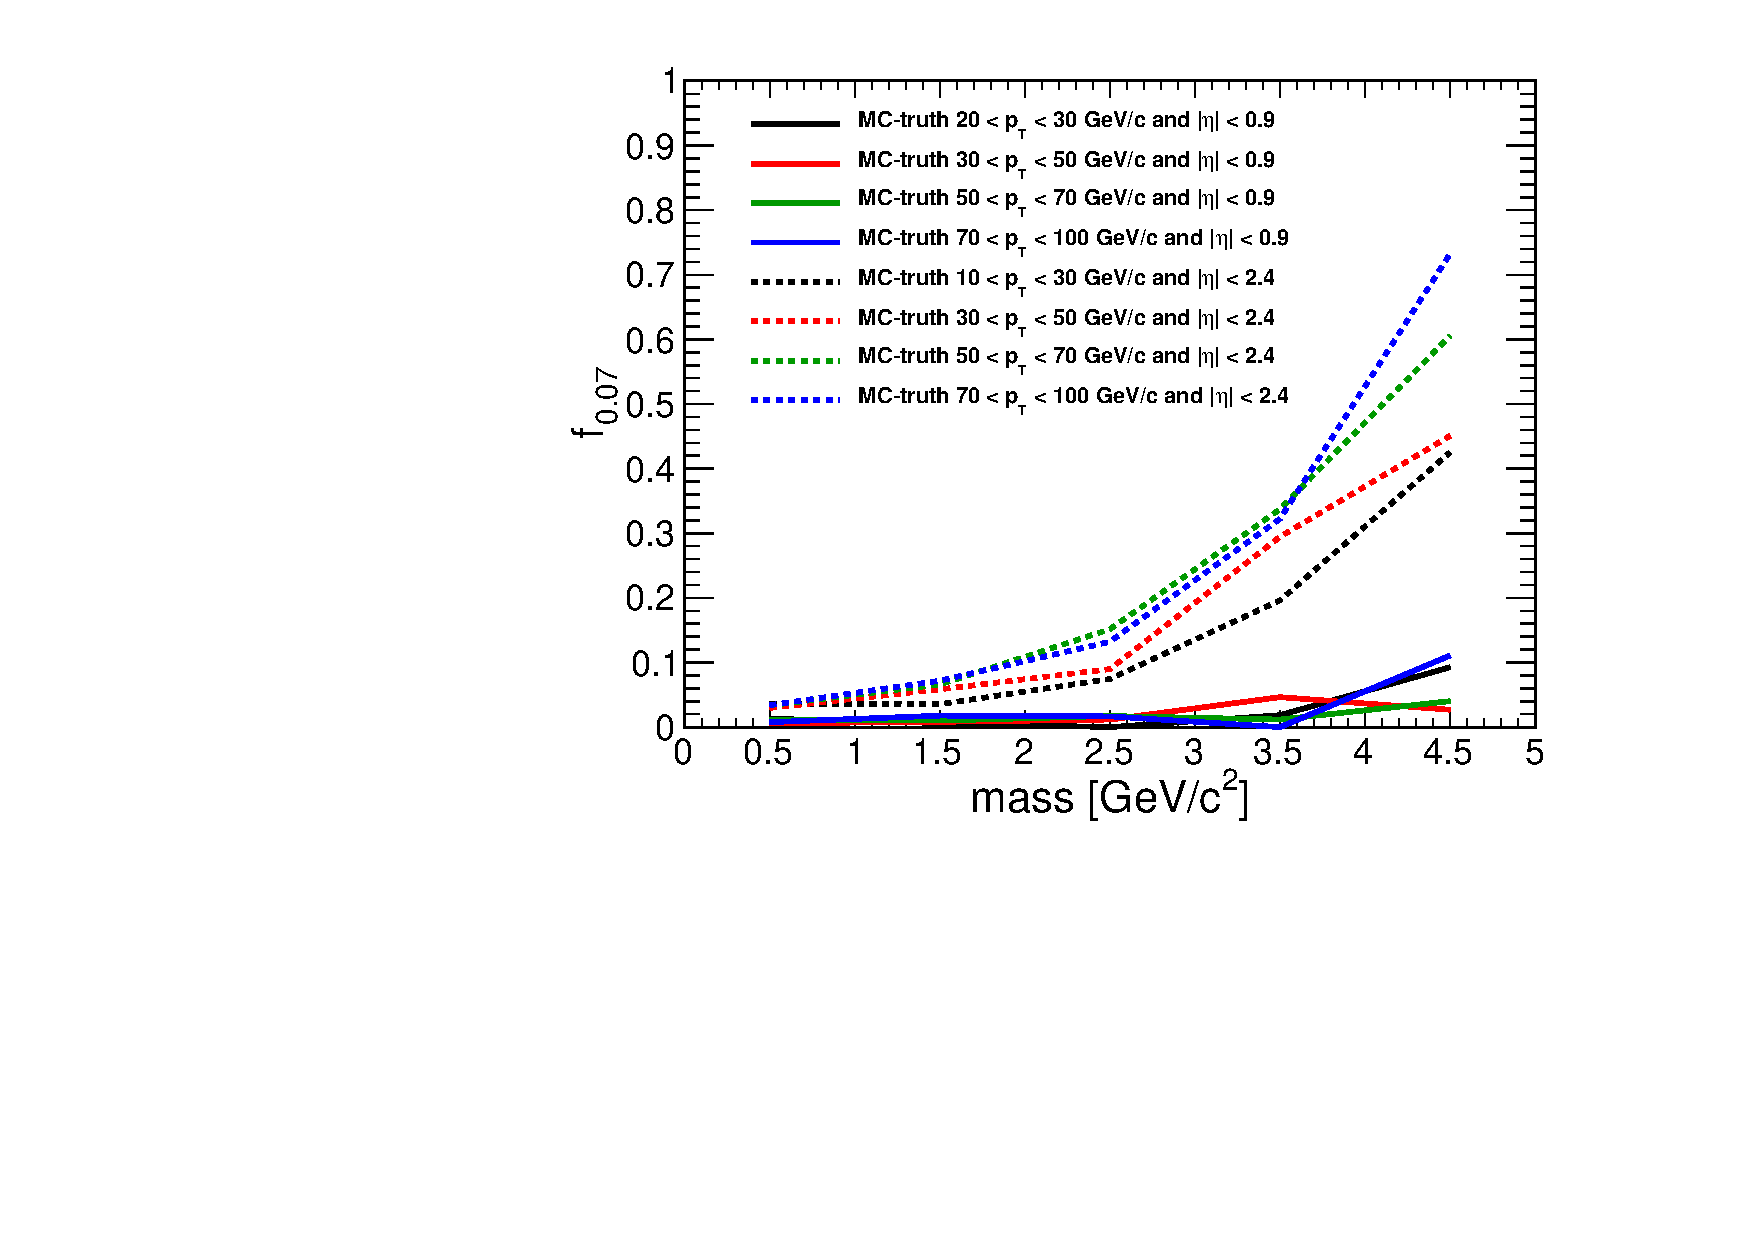
\includegraphics[width=0.5\linewidth]{PLOTS/resolution_f007.pdf}

\caption{Left: resolution as a function of mass for simulated muons
  (lines) and real resonances (points).  Right: the double-Gaussian
  parameter $f_{0.07}$ for simulated muons. \label{fig:resolution}}
\end{figure}

\section{Background estimation}

\subsection{Study of low-mass dimuon spectrum}

\fixme{Move Iso and Lxy stuff to appendix, put all mass plots together}

The shape templates for background mass distributions are derived from
background-enriched samples, in which the Standard Model backgrounds
dominate over any potential signals.  The background-enriched samples
are chosen to have the same physics content as in the signal regions,
which requires a thorough understanding of the background data.  As a
first step, we investigate the 0.25--5~GeV/$c^2$ single-dimuon
spectrum with vector-sum $p_T < 80$~GeV/$c$.
Figure~\ref{fig:support_mass_all} shows a ``raw'' mass spectrum, with
only the following cuts:
\begin{itemize}
\item at least one $p_T > 15$~GeV/$c$, $|\eta| < 0.9$ muon;
\item exactly one additional muon, with $p_T > 5$~GeV/$c$ and $|\eta| < 2.4$;
\item at least one $p_T > 15$~GeV/$c$ L3 muon, to emulate the HLT\_Mu15 trigger.
\end{itemize}
The data are overlaid by Monte Carlo distributions, all scaled to the
integrated luminosity of the dataset (35~pb$^{-1}$).  The following Monte Carlo
samples were used:
\begin{itemize}
\item Drell-Yan, generated by Pythia 8 to avoid an internal mass cut
  in Pythia 6 (with pile-up);
\item prompt $J/\psi \to \mu\mu$, $\psi' \to \mu\mu$, and $\psi' \to
  J/\psi \, \pi\pi \to \mu\mu \, \pi\pi$, produced with Pythia 6,
  decayed with EvtGen, including Photos for final state radiation;
\item inclusive-muons from QCD with $\hat{p}_T > 30$~GeV/$c$,
  generated by Pythia 6 and divided into three partitions:
\begin{itemize}
\item $b\bar{b}$ with one $b$-quark decaying to $\mu\mu X$ by
  double-semileptonic decay or dimuon resonances (both muons have the
  same $B$ hadron as a common ancestor in the generator-level decay
  tree);
\item muons from light-flavor hadronization and muons that are
  unassociated with one another, excluding fakes and decays-in-flight;
\item at least one fake muon and/or decay-in-flight of a charged pion,
  charged kaon, or strange baryon.
\end{itemize}
\end{itemize}

\begin{figure}
\begin{center}
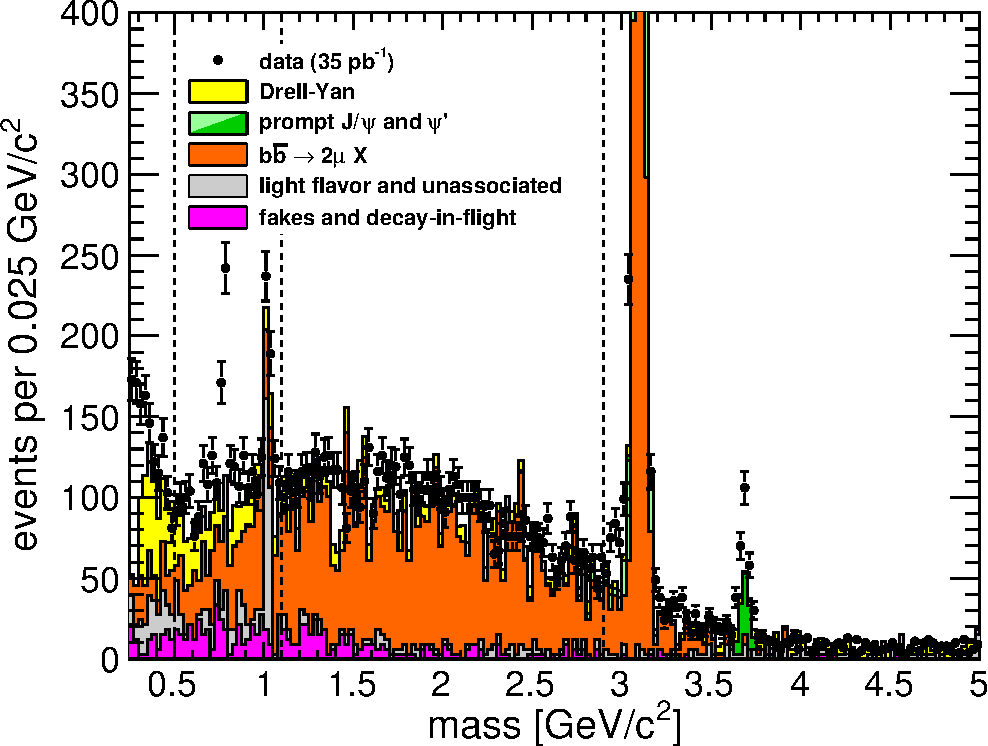
\includegraphics[width=0.5\linewidth]{PLOTS/support_mass_all.pdf}
\end{center}

\caption{Mass distribution of single-dimuon events with Monte Carlo
  simulations superimposed.  (See text for details about the cuts and the
  Monte Carlo samples.) \label{fig:support_mass_all}}
\end{figure}

The two most useful tools for analyzing the physics content of the
distribution are isolation and flight distance.  We define track-based
isolation by
\begin{equation}
Iso = \sum_\s{tracks} p_T \mbox{ if } p_T > 1.5\mbox{ GeV/$c$, }
\Delta R < 0.4 \mbox{, and not a muon,}
\end{equation}
such that the two close-by muons do not veto one another.  The $p_T$
threshold and $\Delta R$ radius were optimized for insensitivity to
pile-up and for a flat distribution near $Iso = 0$ in $b\bar{b}$ Monte
Carlo.  Distributions of $Iso$ for the whole mass distribution,
``continuum'' ($1.1 < \mbox{mass} < 2.9$~GeV/$c^2$), and ``low-mass''
($0.35 < \mbox{mass} < 0.5$~GeV/$c^2$) regions are given in
Fig.~\ref{fig:support_iso}.  (The continuum and low-mass cuts are
indicated by dotted vertical lines in Fig.~\ref{fig:support_mass_all}.)  As
expected, Drell-Yan and prompt resonances are well isolated, while
$b\bar{b}$ is not.

\begin{figure}
\begin{center}
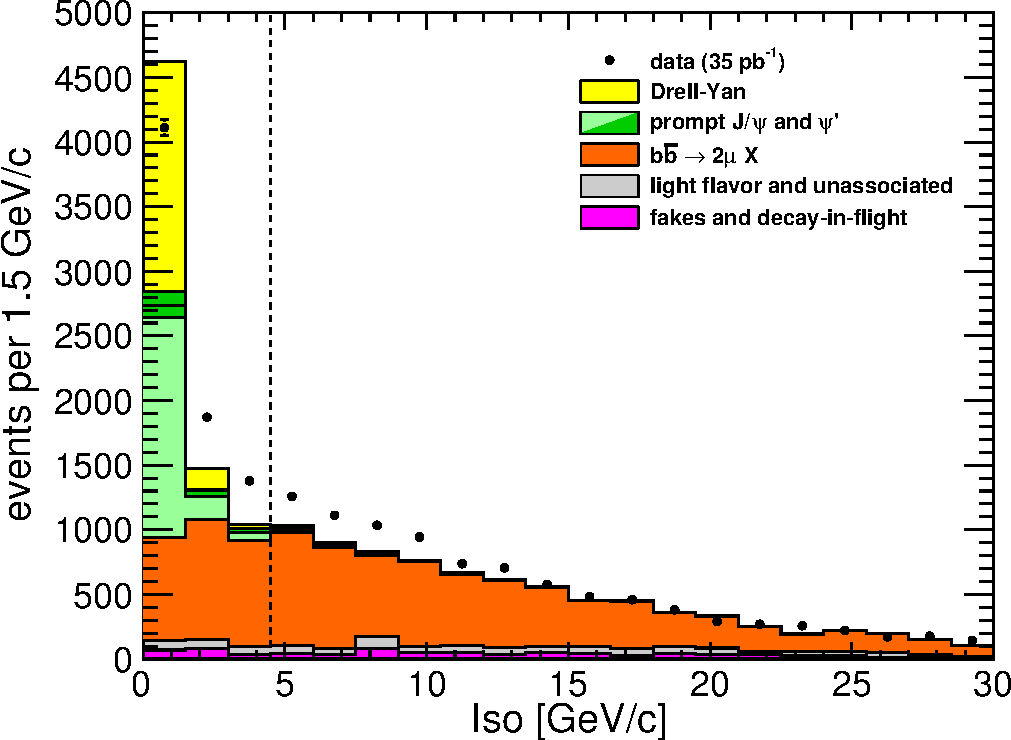
\includegraphics[width=0.5\linewidth]{PLOTS/support_iso_all.pdf}

\vspace{0.35 cm}
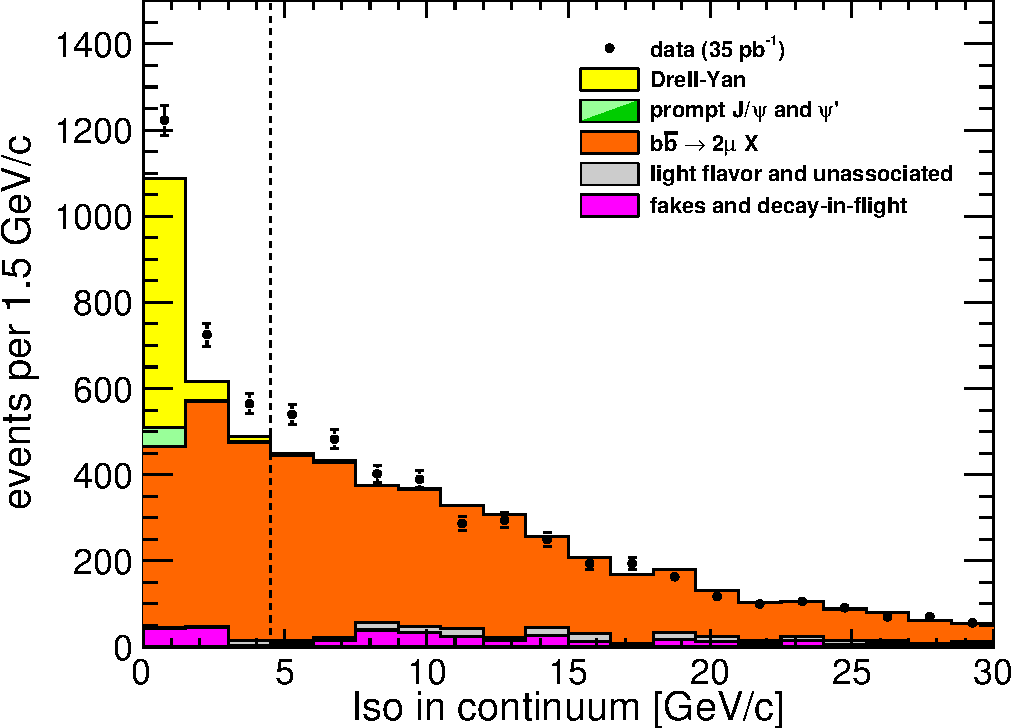
\includegraphics[width=0.48\linewidth]{PLOTS/support_iso_continuum.pdf}
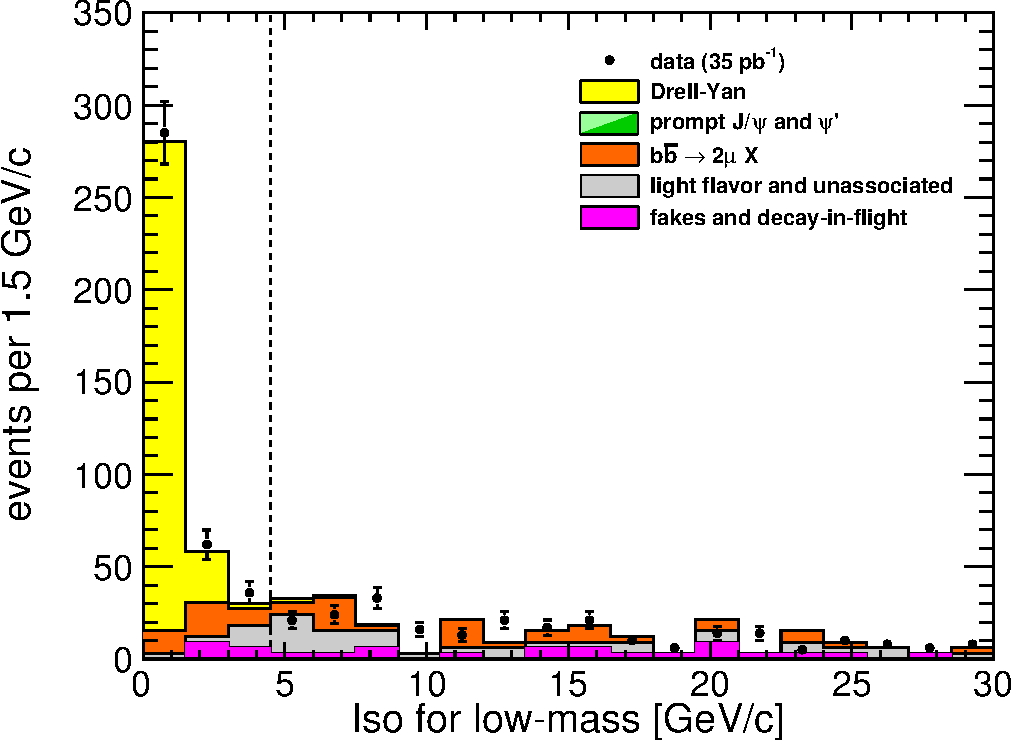
\includegraphics[width=0.48\linewidth]{PLOTS/support_iso_lowmass.pdf}
\end{center}

\caption{Track-based isolation (see text for definition) for the
  whole sample (top), 1.1--2.9~GeV/$c^2$ continuum (bottom-left), and
  0.35--0.5~GeV/$c^2$ low-mass region (right). \label{fig:support_iso}}
\end{figure}

The flight distance is defined as
\begin{equation}
L_{xy} = \frac{(v_x - V_x) p_x + (v_y - V_y) p_y}{\sqrt{{p_x}^2 + {p_y}^2}}
\end{equation}
where ($v_x$, $v_y$) is the 2-D position of the dimuon vertex, ($p_x$,
$p_y$) is the 2-D projection of the dimuon momentum vector, and
($V_x$, $V_y$) is the 2-D position of the closest primary vertex in
the $z$ direction ($z$ is parallel with the beamline).
Figure~\ref{fig:support_lxy} shows distributions of $L_{xy}$ in the
same mass bins as isolation.  Vertices with negative $L_{xy}$ are
mis-measured; this provides a direct indication of the vertex
resolution.  Drell-Yan and prompt resonances form a peak centered on
$L_{xy} = 0$, while $b\bar{b}$ has a long tail toward positive
$L_{xy}$ due to the long lifetimes of $B$ hadrons.  Vertex resolution
degrades when the opening angle is small, which is why the symmetric
peak in the low-mass bin is wider than in all other bins.

\begin{figure}
\begin{center}
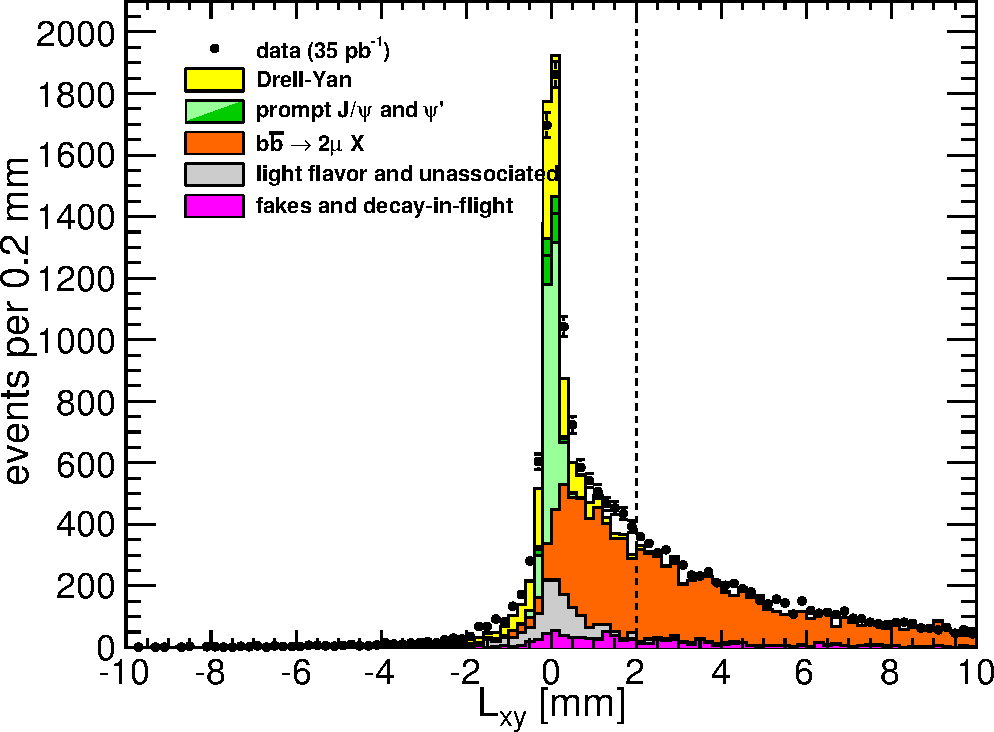
\includegraphics[width=0.5\linewidth]{PLOTS/support_lxy_all.pdf}

\vspace{0.35 cm}
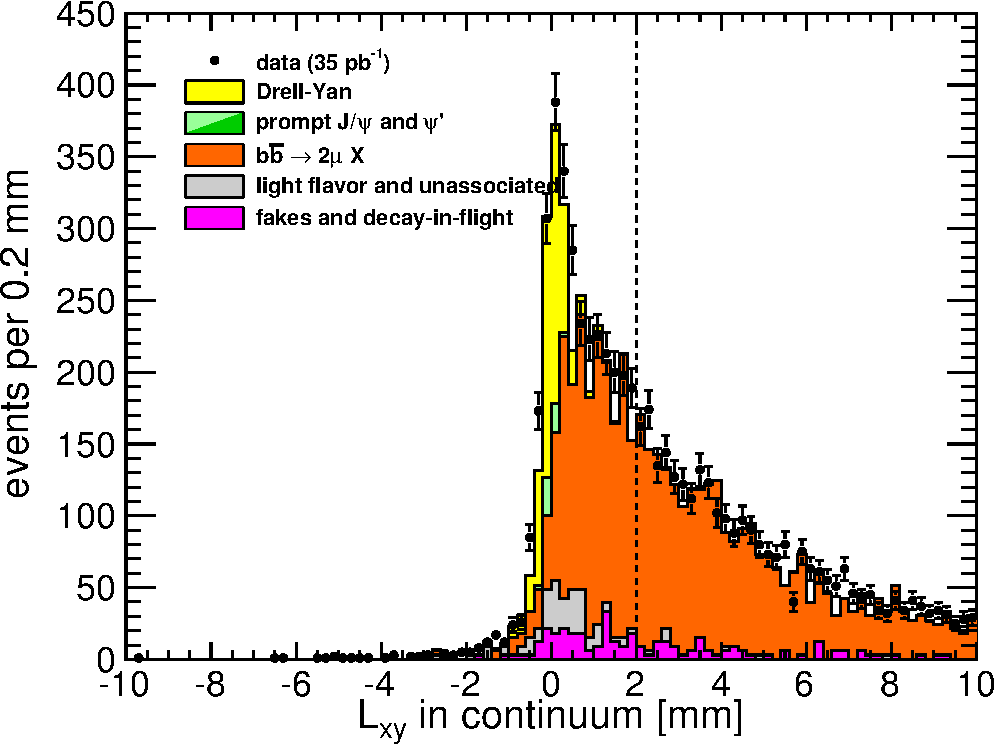
\includegraphics[width=0.48\linewidth]{PLOTS/support_lxy_continuum.pdf}
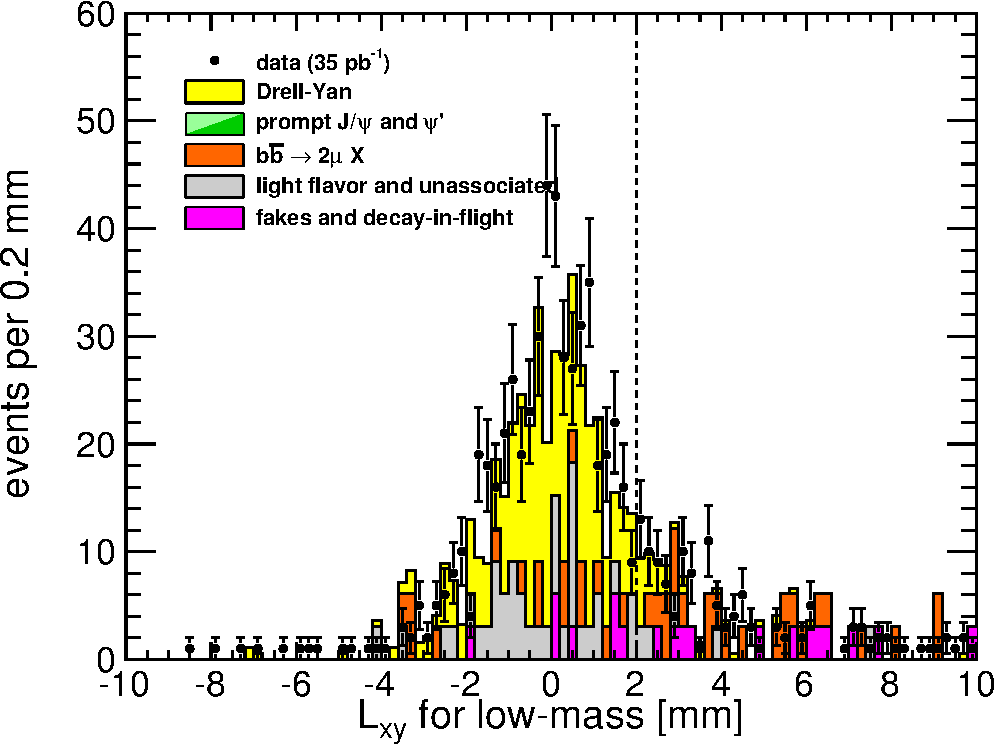
\includegraphics[width=0.48\linewidth]{PLOTS/support_lxy_lowmass.pdf}
\end{center}

\caption{Distance of the dimuon vertex (in $x$-$y$) from the closest
  primary vertex (in $z$), along the direction of the dimuon momentum
  axis, for the whole sample (top), 1.1--2.9~GeV/$c^2$ continuum
  (bottom-left), and 0.35--0.5~GeV/$c^2$ low-mass region
  (right).  \label{fig:support_lxy}}
\end{figure}

From $Iso$ an $L_{xy}$, we can see that the two major components of
the data are $b\bar{b}$ and prompt/Drell-Yan, each containing
resonance and continuum contributions.  We can partition the sample
using the following ``$b\bar{b}$ cuts,''
\begin{equation}
Iso > 4.5\mbox{ GeV/$c$ {\bf or }} L_{xy} > \mbox{2 mm.}
\label{eqn:bbcuts}
\end{equation}
These threshold are indicated with dotted vertical lines in
Figs.~\ref{fig:support_iso} and \ref{fig:support_lxy}.  The invariant
mass distribution with $b\bar{b}$ and anti-$b\bar{b}$ cuts is shown in
Fig.~\ref{fig:support_mass}.  The inclusive-muon sample is missing
$\omega$ and $\psi'$ resonances, while the prompt/Drell-Yan is missing
only the $\omega$.  Most of the dimuons arising from fakes and
decays-in-flight pass the $b\bar{b}$ cut, comprising about 25\% of the
events passing the cut below 1~GeV/$c^2$.  Below 0.5~GeV/$c^2$, there
is a low-mass rise not described by the Monte Carlo, and this
distribution is to wide to be a detector resolution-dominated $\mu\mu$
resonance.

\begin{figure}
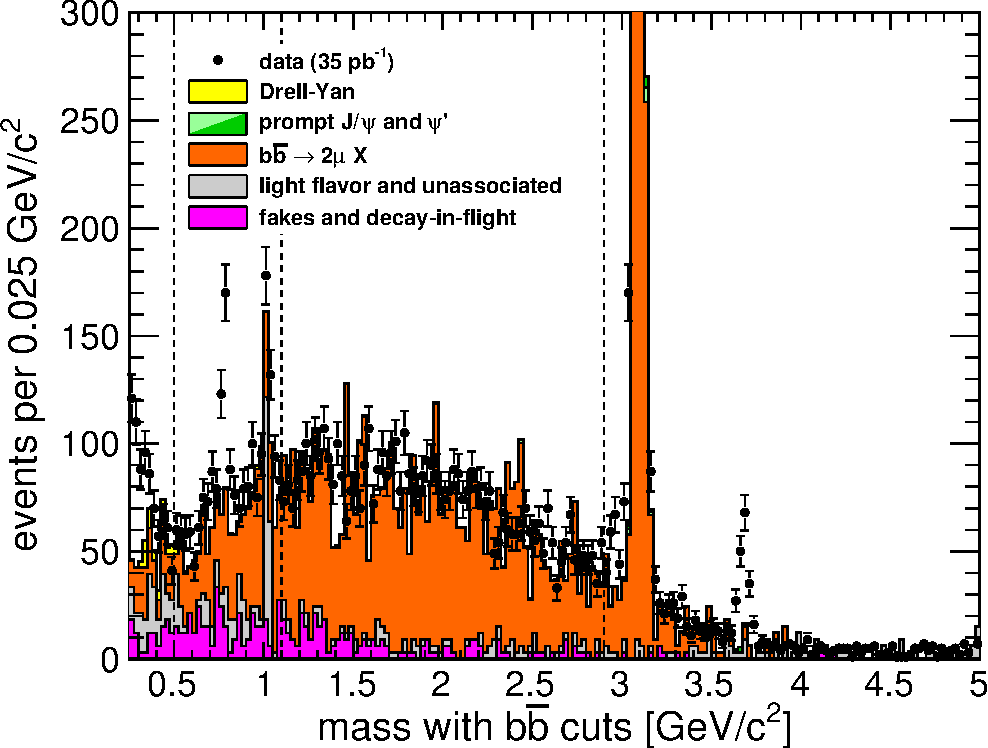
\includegraphics[width=0.5\linewidth]{PLOTS/support_mass_bbbar.pdf}
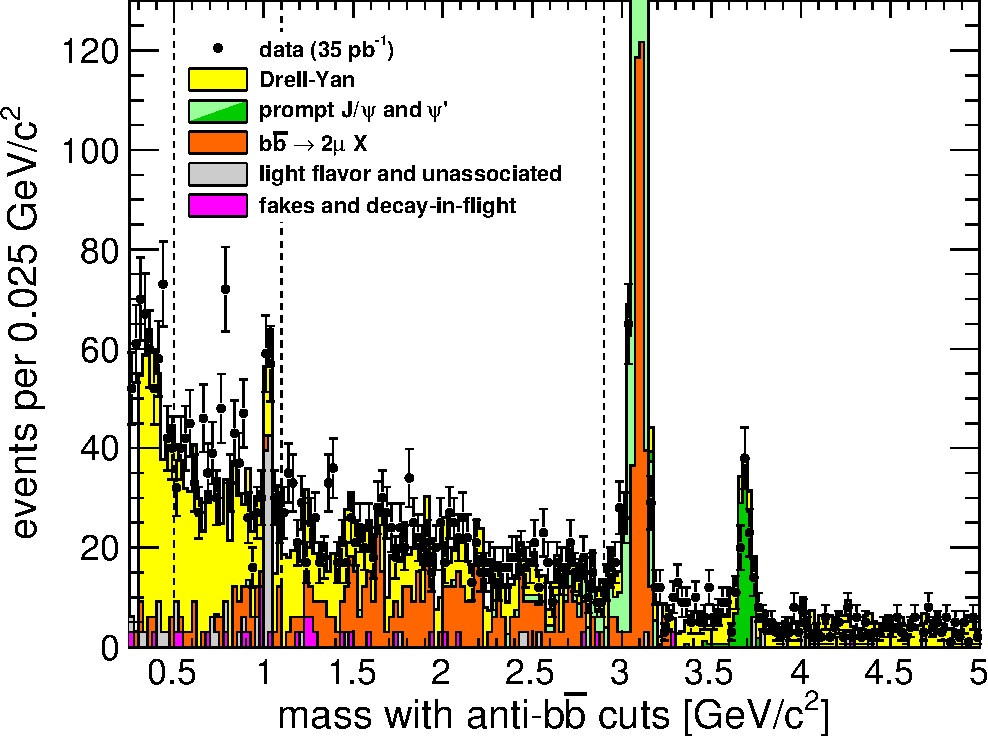
\includegraphics[width=0.5\linewidth]{PLOTS/support_mass_antibbbar.pdf}

\caption{The mass distribution partitioned by $b\bar{b}$ cuts. \label{fig:support_mass}}
\end{figure}

\fixme{Everything about the eta goes to the appendix}

The low-mass rise has an endpoint near the $\eta$ mass
(0.55~GeV/$c^2$), and $\eta$ has a large branching fraction to
$\mu\mu\gamma$ ($3\times 10^{-4}$, which is comparable to branching
fractions for $\omega \to \mu\mu$ and $\phi \to \mu\mu$), which is
much larger than its branching fraction to $\mu\mu$ ($6\times
10^{-6}$).  We therefore consider that the low-mass rise might be
$\eta \to \mu\mu\gamma$ events reconstructed without the photon, and
attempt to find the photon.  Figure~\ref{fig:eta_peak} shows a
$\mu\mu\gamma$ invariant mass and a close-up of the $\mu\mu$ invariant
mass, both with $b\bar{b}$ cuts.  The photons are reconstructed using
the particle-flow photon algorithm, and exactly one is required within
$\Delta R < 0.1$ of the dimuon axis.  A significant $\eta$ peak
containing 63$\pm$15 $\eta \to \mu\mu\gamma$ events is observed in
$\mu\mu\gamma$, compared to about 170 in the $\mu\mu$ low-mass rise.
\fixme{Need to know the efficiency of finding $\mu\mu\gamma$ with this
  technique compared to the efficiency of finding $\mu\mu$.  It is
  important that the photon-finding efficiency is evaluated {\it in
    jets.}}  At least 1/3 of the low-mass rise is due to the $\eta$
resonance.

\begin{figure}
\mbox{ } \hfill 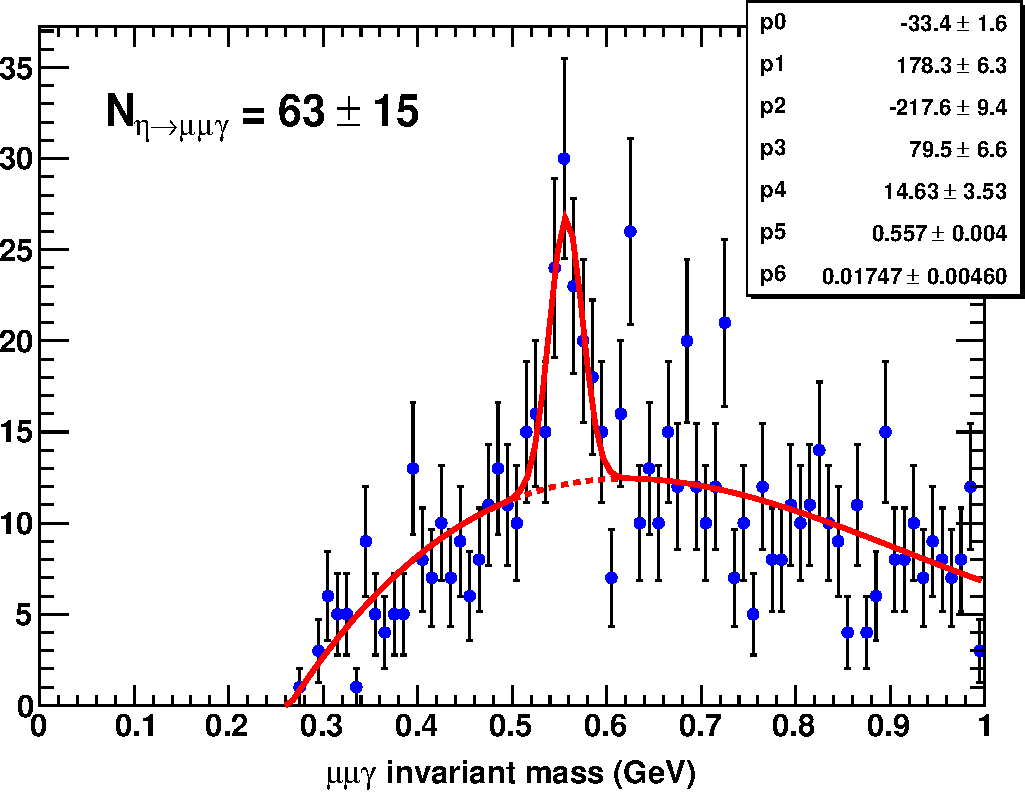
\includegraphics[height=6.4 cm]{PLOTS/eta_peak.pdf} \hfill
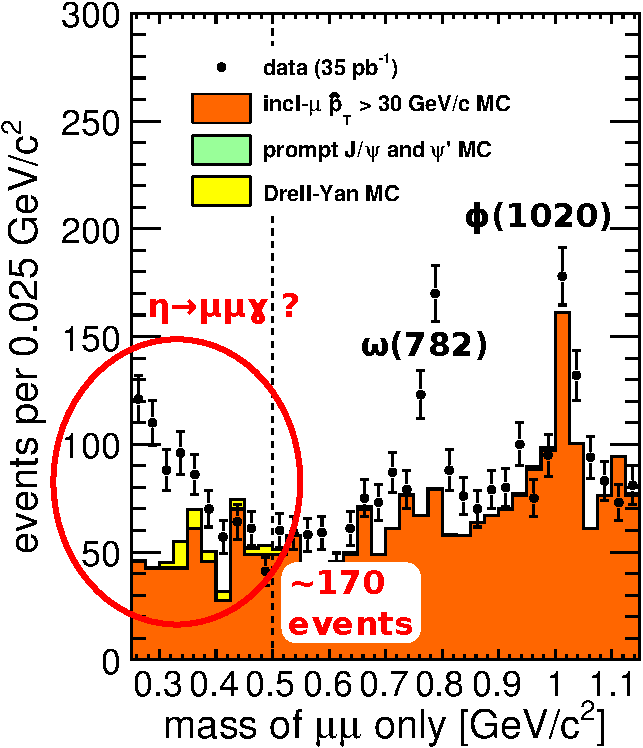
\includegraphics[height=6.4 cm]{PLOTS/mass_of_mumu_only.pdf} \hfill \mbox{ }

\caption{Left: three-body $\mu\mu\gamma$ mass distribution, in which
  exactly one particle-flow photon is required within $\Delta R < 0.1$
  of the dimuon axis.  Right: a close-up of the low-mass excess in
  $\mu\mu$ with the same cuts. \label{fig:eta_peak}}
\end{figure}

\subsection{Mass template for (a-1): high-$p_T$ dimuons}

The (a-1) signal region, exactly one dimuon with vector-sum $p_T >
80$~GeV/$c$, has a mass template derived from low-momentum dimuons.
For a background-enriched sample, we use dimuons with $40 < p_T <
60$~GeV/$c$, and then test it in a $60 < p_T < 80$~GeV/$c$ control
sample.  The control sample is also background-dominated for $\lesssim
1$~pb signals, but it is closer in kinematics to the signal region.

The choice of 40--60 and 60--80~GeV/$c$ regions is motivated by the
fact that the major components of the data scale proportionally with
$p_T$ above 40~GeV/$c$.  Figure~\ref{fig:support_bbbarcut_limits}
shows the $p_T$ distribution of the data partitioned into three
classes:
\begin{itemize}
\item non-$J/\psi$ events passing the $b\bar{b}$ cuts;
\item $J/\psi$ events passing the $b\bar{b}$ cuts;
\item events failing the $b\bar{b}$ cuts;
\end{itemize}
where $J/\psi$ events are selected with a 0.15~GeV/$c^2$-wide mass
window around the PDG $J/\psi$ mass.  Each of these three
distributions is exponential with mutually consistent length scales:
$k = 9.93\pm0.36$, $10.04\pm0.54$, and $9.94\pm0.57$ for the three
classes respectively when fitted to $A\exp(-x/k)$.  In the
accompanying figure, the shape of the 40--60~GeV/$c$ mass distribution
(without $b\bar{b}$ cuts) is overlaid on the 60--80~GeV/$c$ mass
distribution, and they appear to be consistent.  To verify that this
consistency in shape continues into the signal region, we plot
inclusive-muon Monte Carlo mass distributions in 20~GeV/$c$ bins of
$p_T$ from 40 to 120~GeV/$c$.

\begin{figure}
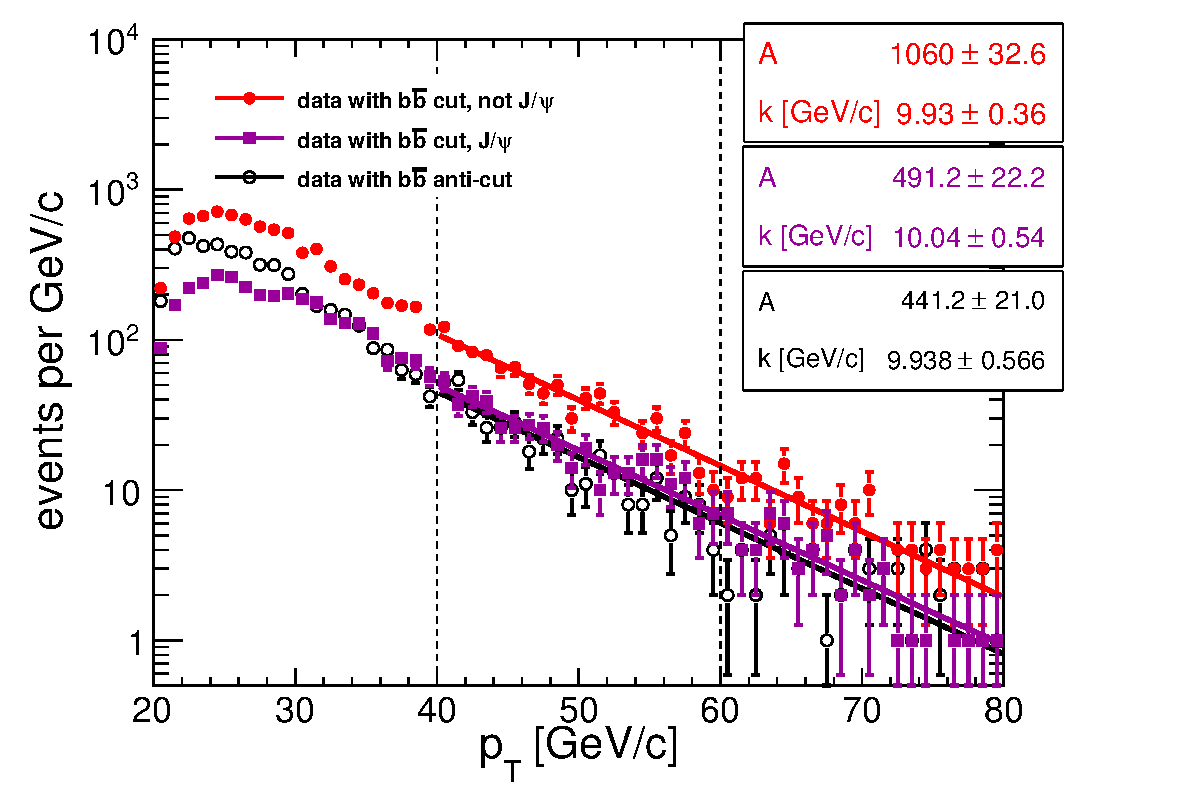
\includegraphics[width=0.5\linewidth]{PLOTS/support_bbbarcut_limits.pdf}
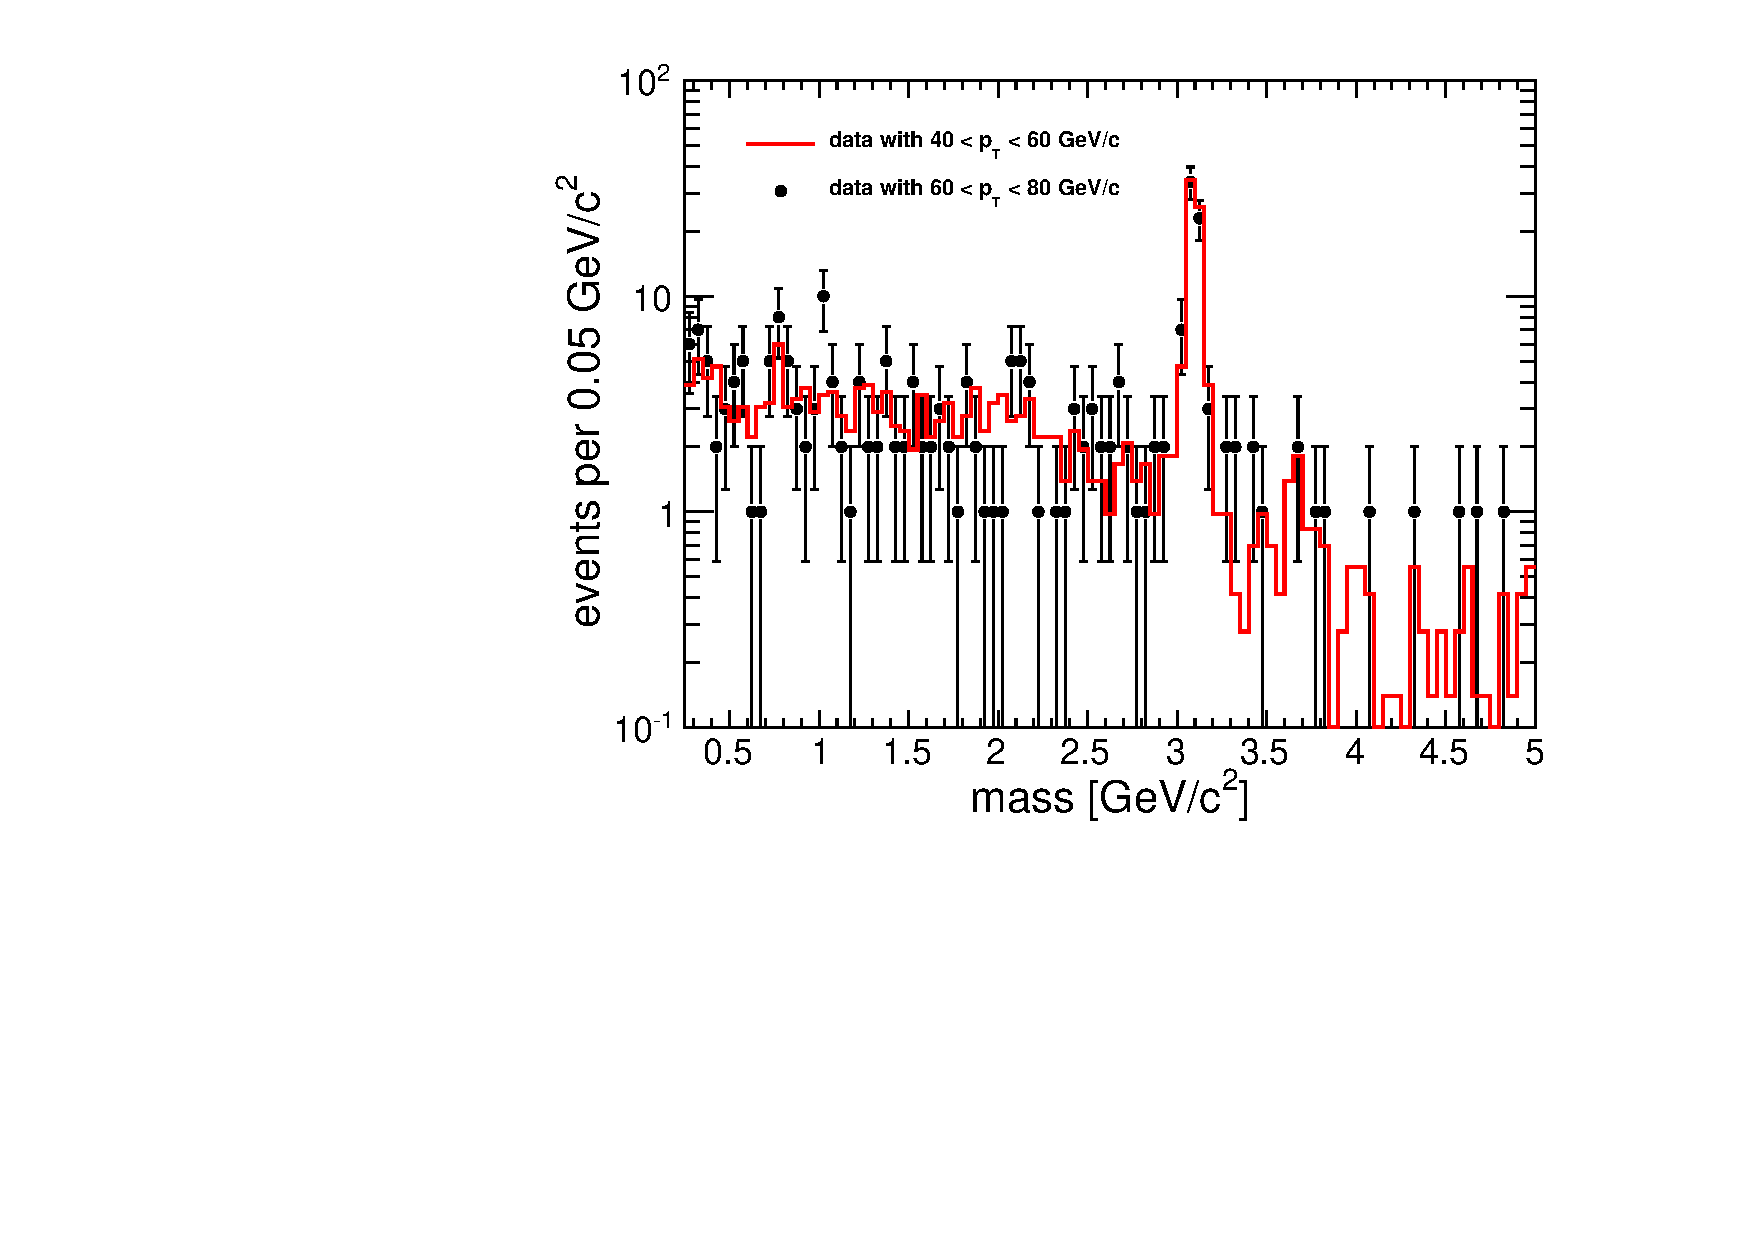
\includegraphics[width=0.5\linewidth]{PLOTS/support_limits_mass.pdf}

\caption{Scaling of single-dimuon data with $p_T$.  Left: $p_T$
  spectra for three non-overlapping subsamples of dimuons ($\propto
  \exp(-x/k)$, normalized by $A$, the integral from 40 to 80~GeV/$c$).
  Right: mass spectrum in two bins of $p_T$, scaled to equal
  area. \label{fig:support_bbbarcut_limits}}
%% %% \begin{equation}
%% %% \frac{A \exp(-x/k)}{k (\exp(-\mbox{40 GeV/$c$}/k) - \exp(-\mbox{80 GeV/$c$}/k))}
%% %% \end{equation}
\end{figure}

\begin{figure}
\begin{center}
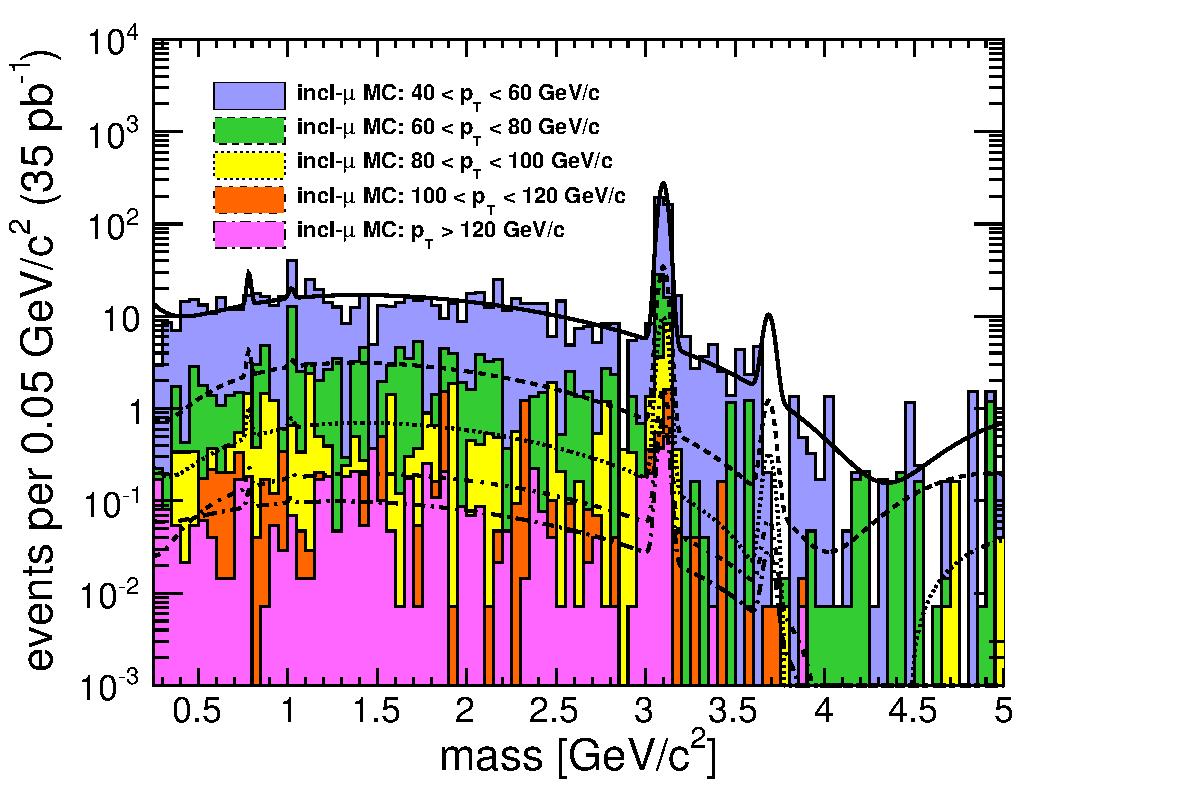
\includegraphics[width=0.6\linewidth]{PLOTS/support_mass_vs_pt.pdf}
\end{center}

\caption{Mass distribution of inclusive-muon MC in bins of $p_T$ from
  40 to 120~GeV/$c$. \label{fig:support_mass_vs_pt}}
\end{figure}

The template shape for the (a-1) region is obtained by fitting the
40--60~GeV/$c$ mass distribution to the following curve:
\begin{multline}
B(m; p_R, f_\omega, f_\phi, f_\psi, f_m, p_{-1}, p_0, p_1, p_2, p_3, p_4) = 
p_R \bigg[f_\omega \, G(m; 0.78265, 0.011) + \\ f_\phi \, G(m; 1.019455, 0.014) + G(m; 3.096916, 0.025) + f_{\psi'} \, G(m; 3.68609, 0.029) + \frac{f_m}{m} \bigg] \\
+ \frac{p_{-1}}{m} + p_0 + p_1 (m - 5) + p_2 (m - 5)^2 + p_3 (m - 5)^3 + p_4 (m - 5)^4.
\label{eqn:bkgnd_shape}
\end{multline}
The $p_R$ parameter normalizes all resonances, with $f_\omega$,
$f_\phi$, $f_{\psi'}$, and $f_m$ normalizing the individual resonances
with respect to the $J/\psi$.  The function $G(m; m_0, \sigma)$ is a
Gaussian with $m_0$ (centroid) and $\sigma$ (resolution) in GeV/$c^2$.
For each resonance, $m_0$ is fixed to its PDG mass and $\sigma$ is
fixed to the resolution obtained in
Sec.~\ref{sec:signal_mass_spectrum_shape}.  The $f_m$ term describes
the low-mass rise, categorized here as a resonance because of its
large $\eta \to \mu\mu\gamma$ component.  The $p_{-1}$, $p_0$, $p_1$,
$p_2$, $p_3$, $p_4$ terms are an expansion of the background shape as
a Taylor/Laurent polynomal.  For the (a-1) region, $p_{-1}$ is fixed
to zero.  Figure~\ref{fig:backgroundEnriched_highpt} shows a fit of
the background-enriched data to this shape, and an overlay of the
shape on the control region.

\begin{figure}
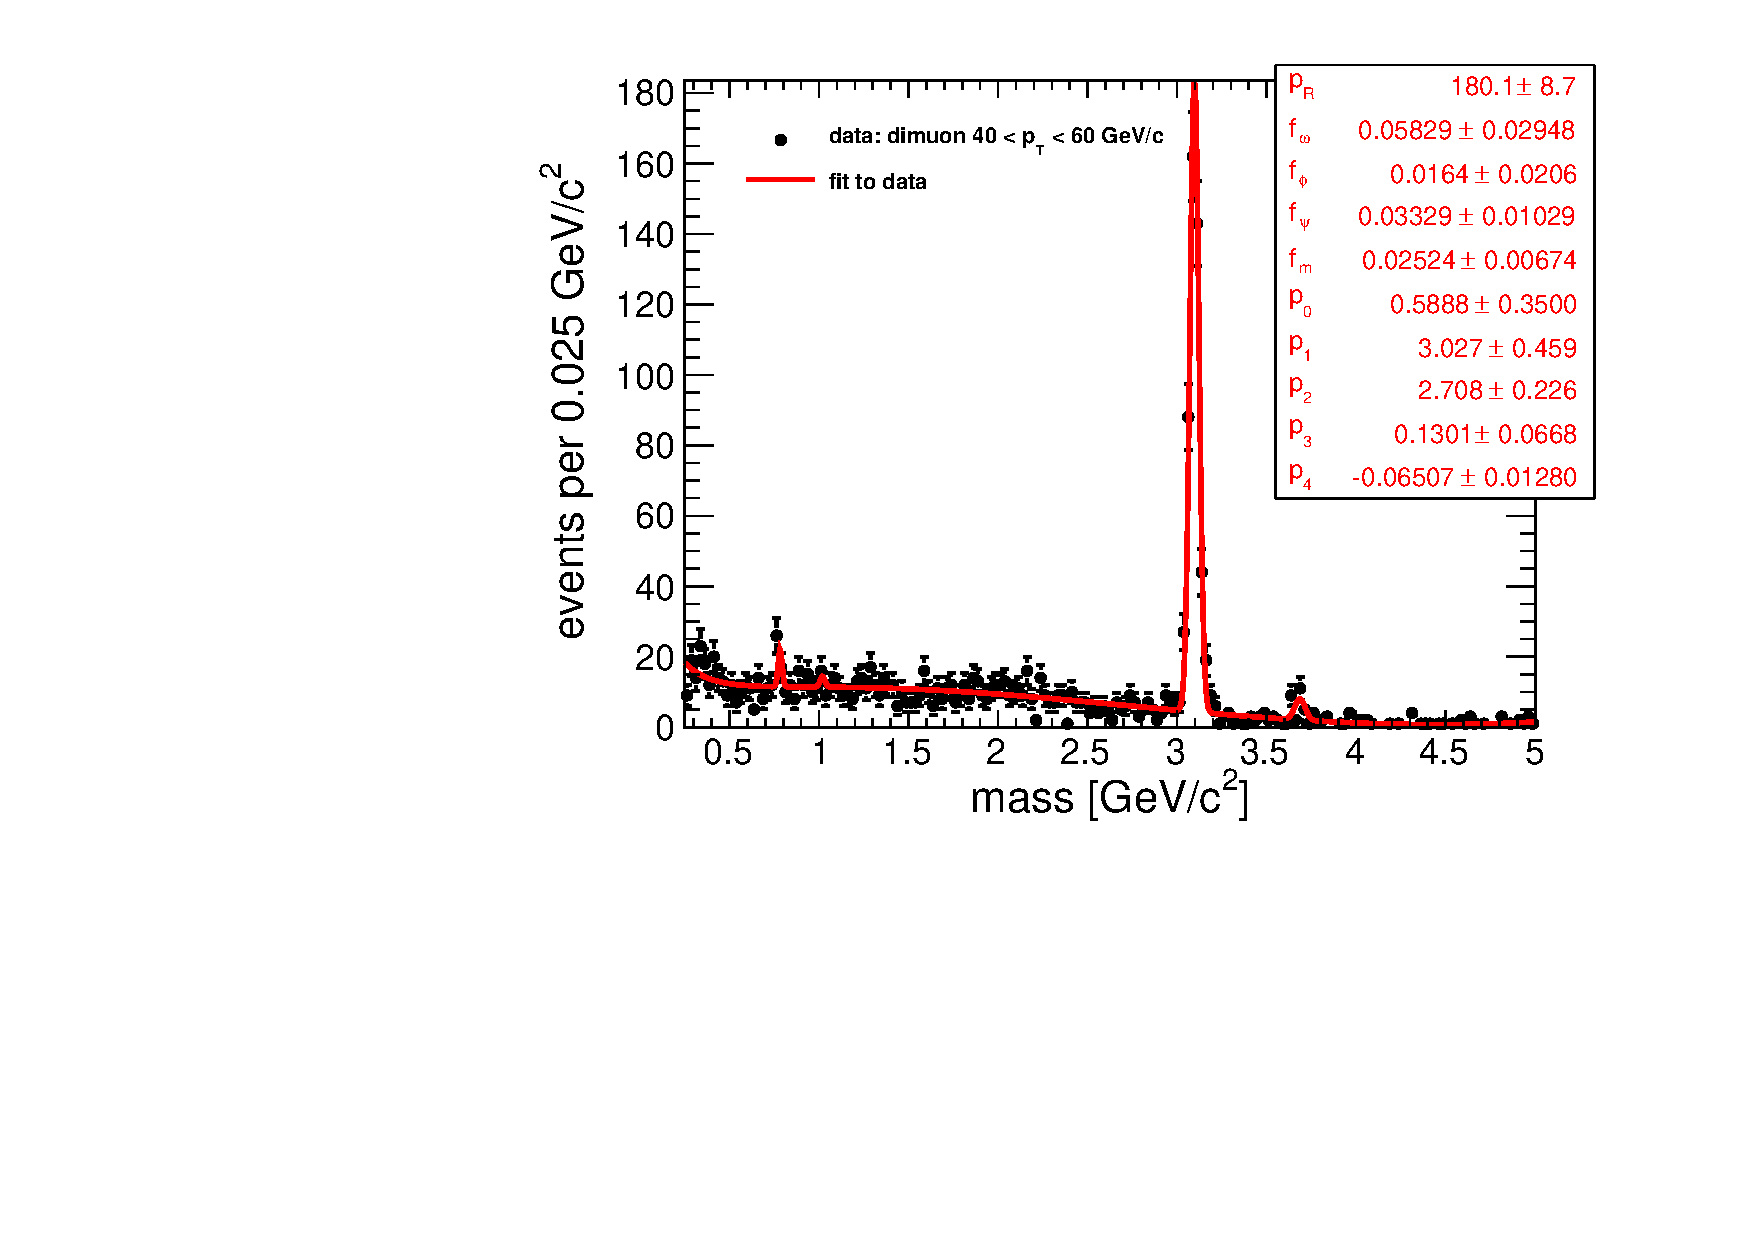
\includegraphics[width=0.5\linewidth]{PLOTS/fullscale-backgroundEnriched_highpt.pdf}
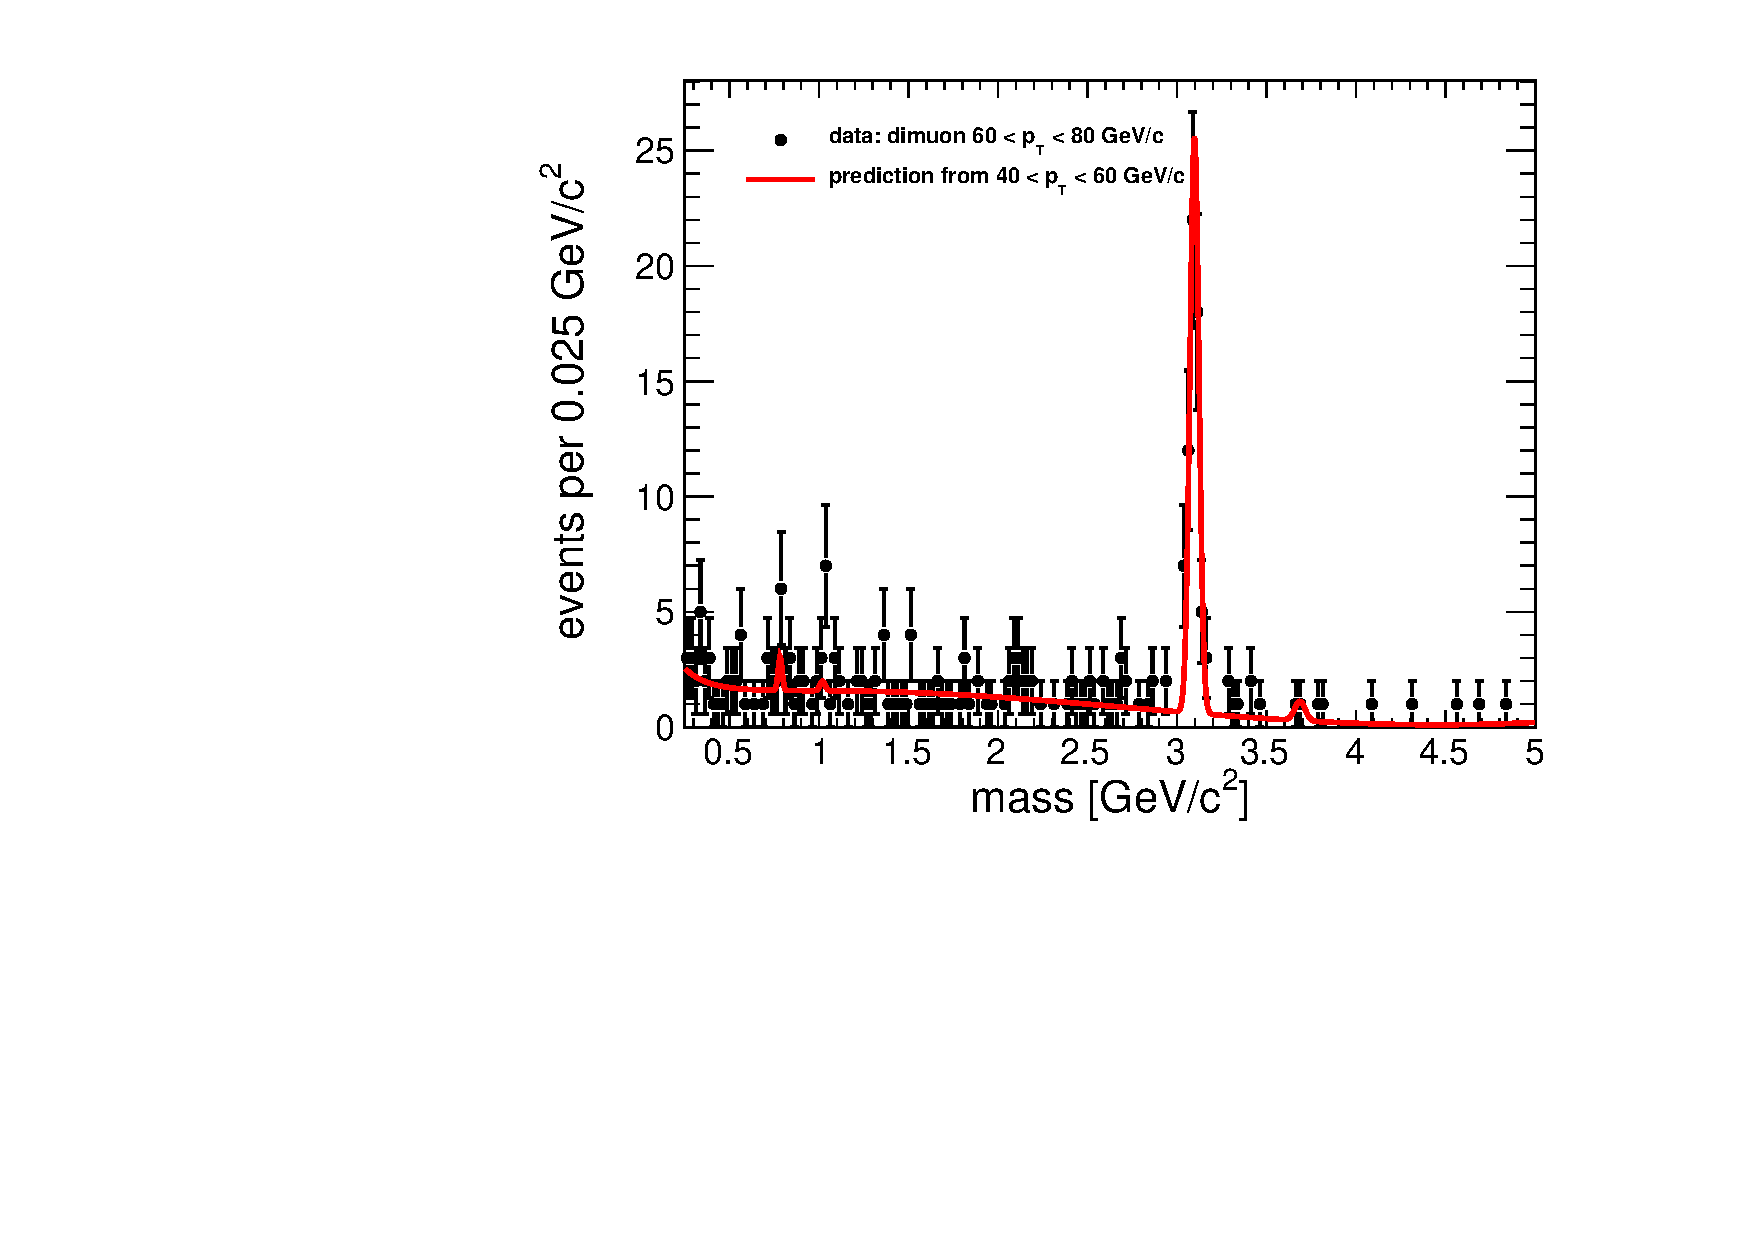
\includegraphics[width=0.5\linewidth]{PLOTS/fullscale-control_highpt.pdf}

\caption{Left: fit of the (a-1) background-enriched data to
  Eqn.~\ref{eqn:bkgnd_shape}.  Right: overlay of the same shape on the
  corresponding control region. \label{fig:backgroundEnriched_highpt}}
\end{figure}

\subsection{Mass template for (a-2) and (a-3): high-multiplicity mu-jets}

The (a-2) signal region consists of exactly one neutral mu-jet with
four muons, and the (a-3) region is exactly one mu-jet with more than
four muons.  Standard Model processes that yield these topologies with
real muons are rare (primarily boosted $b\bar{b}$), so the dominant
backgrounds are mu-jets containing fake and decay-in-flight muons.
``Fake'' muons are rare failures of the muon identification procedure,
in which muon chamber segments from one real muon are assigned to two
distinct tracks in the tracker.  Decays-in-flight are $\pi^\pm \to
\mu^\pm\nu$, $K^\pm \to \mu^\pm \nu$, and (less frequently) strange
baryons producing a muon far from the primary and secondary vertices.
Dimuons containing a fake or a decay-in-flight muon typically have low
mass distributions, peaking at 1~GeV/$c^2$ as shown in
Fig.~\ref{fig:mc_mass_spectra_fakes}.  The distributions are similar
because in both cases, a real muon is paired with a random hadronic
particle.

\begin{figure}
\begin{center}
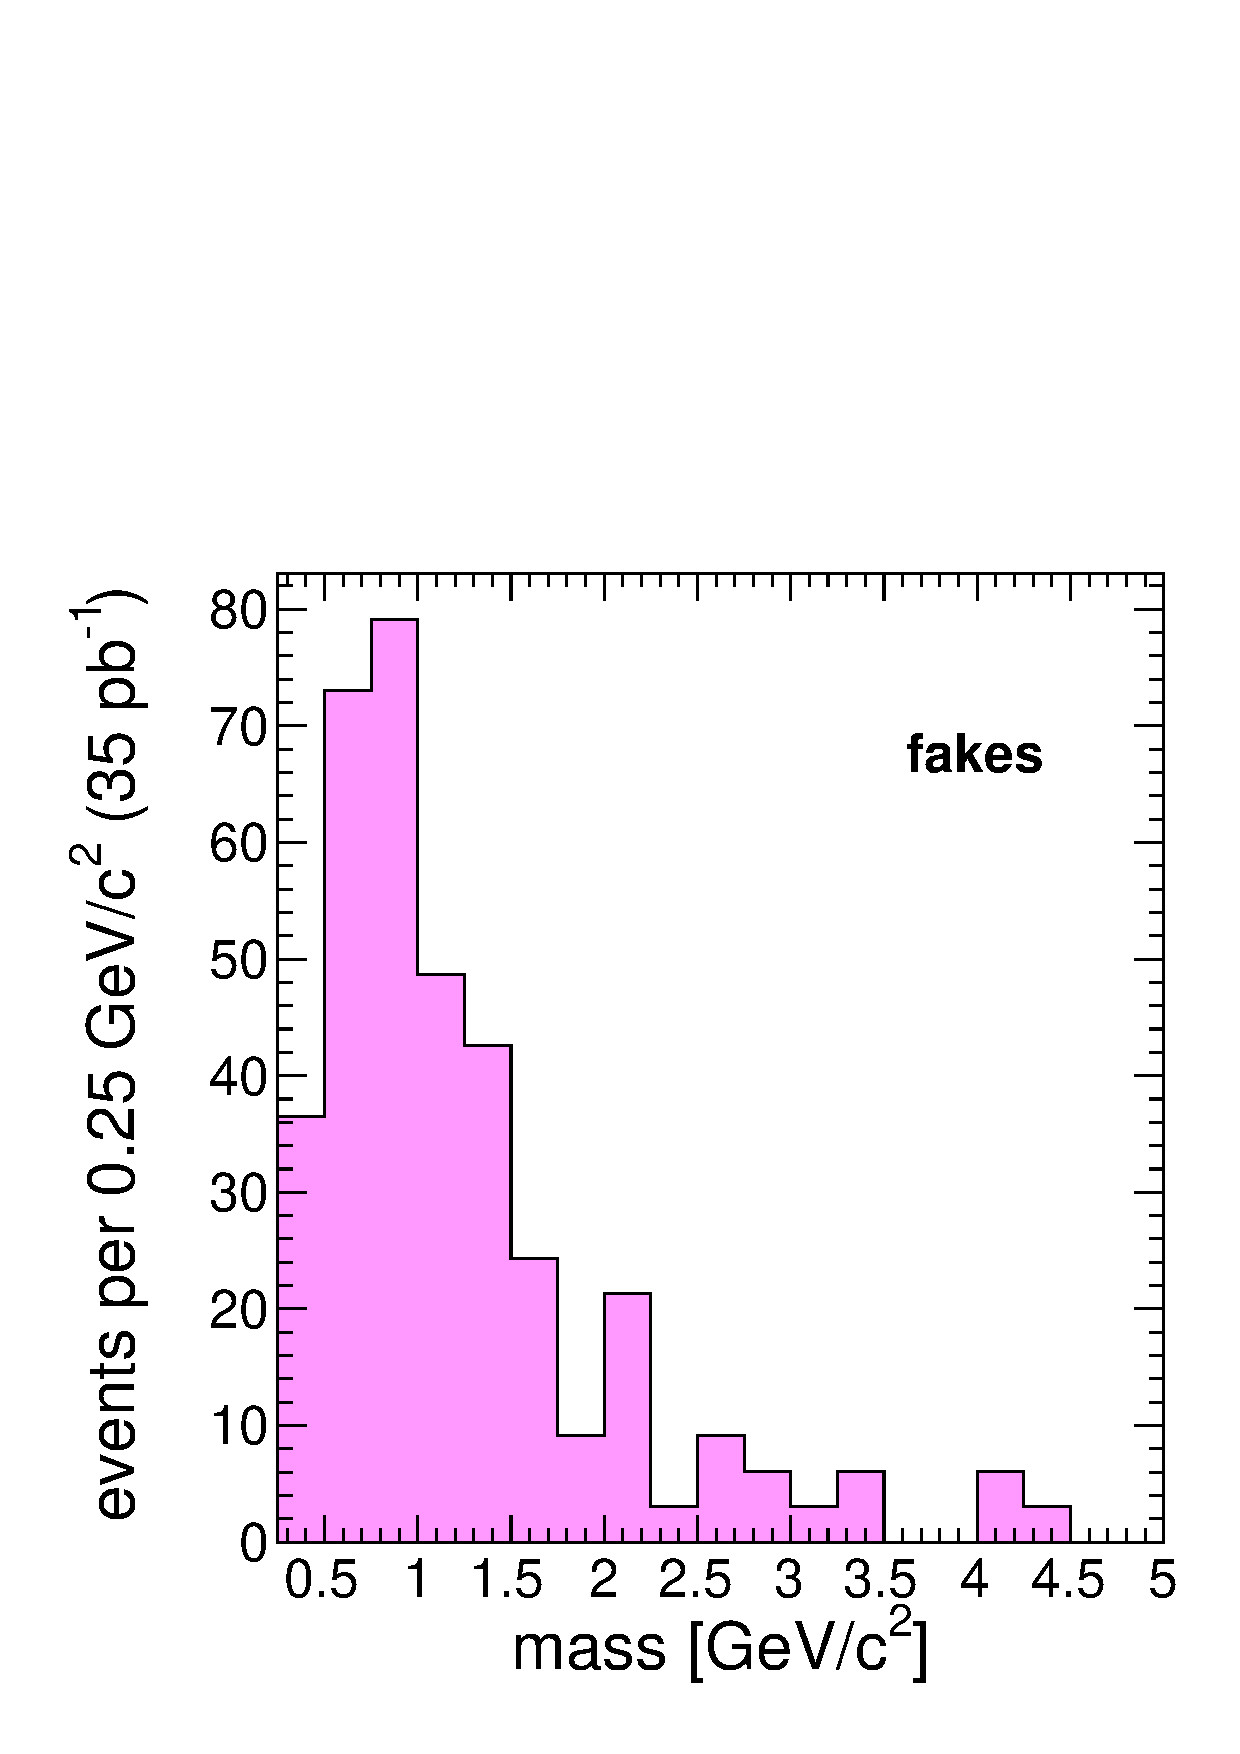
\includegraphics[width=0.3\linewidth]{PLOTS/mc_mass_spectra_onlyfakes.pdf} \hspace{0.25 cm}
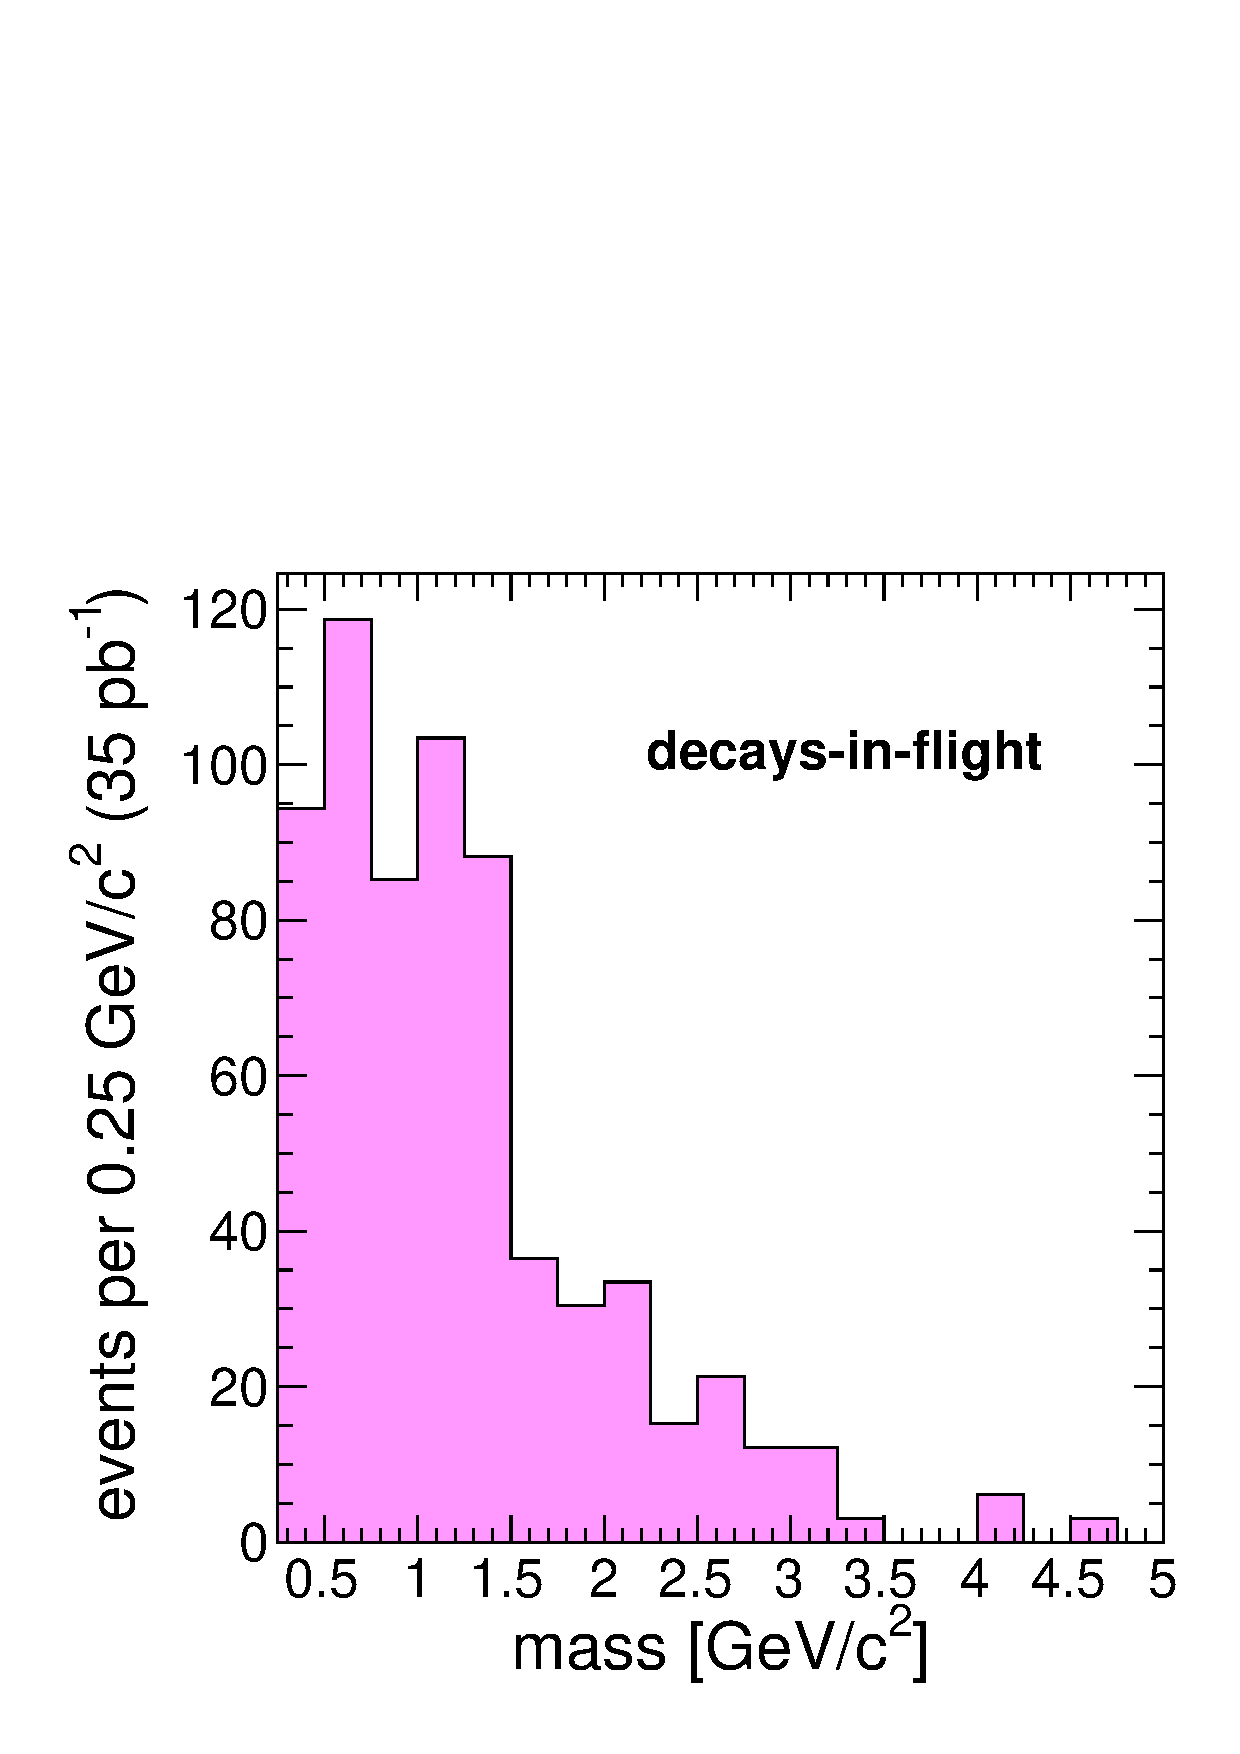
\includegraphics[width=0.3\linewidth]{PLOTS/mc_mass_spectra_onlyinflights.pdf}
\end{center}

\caption{Distributions of dimuon mass for dimuons containing fake and
  decay-in-flight muons in inclusive-muon Monte
  Carlo. \label{fig:mc_mass_spectra_fakes}}
\end{figure}

The shape of the dimuon mass distribution with a fake or
decay-in-flight muon can be quantified using data by pairing real
muons with random hadronic tracks.  We search for tracks near mu-jets
with the same properties as quality TrackerMuons, except that no
requirement is made on the muon chamber segments.  We require the
track to satisfy:
\begin{itemize}
\item $p_T > 5$~GeV/$c$ and $|\eta| < 2.4$;
\item number of hits $\ge$ 8;
\item $\chi^2/N_\s{DOF} < 4$;
\end{itemize}
and the track at at least one muon in the mu-jet must satisfy:
\begin{itemize}
\item opposite charge;
\item invariant mass $<$ 5~GeV/$c^2$;
\item vertex probability $>$ 1\%;
\item $\Delta R < 0.01$ if either of the above fail (including vertex
  reconstruction).
\end{itemize}
Thus, the extra track or tracks have the same distributions as muons
in a mu-jet, with the exception of muon chamber segments.
Figure~\ref{fig:support_mujetplustracks_ptspectra} shows the $p_T$
distributions of muons and extra tracks in these samples.

\begin{figure}
\begin{center}
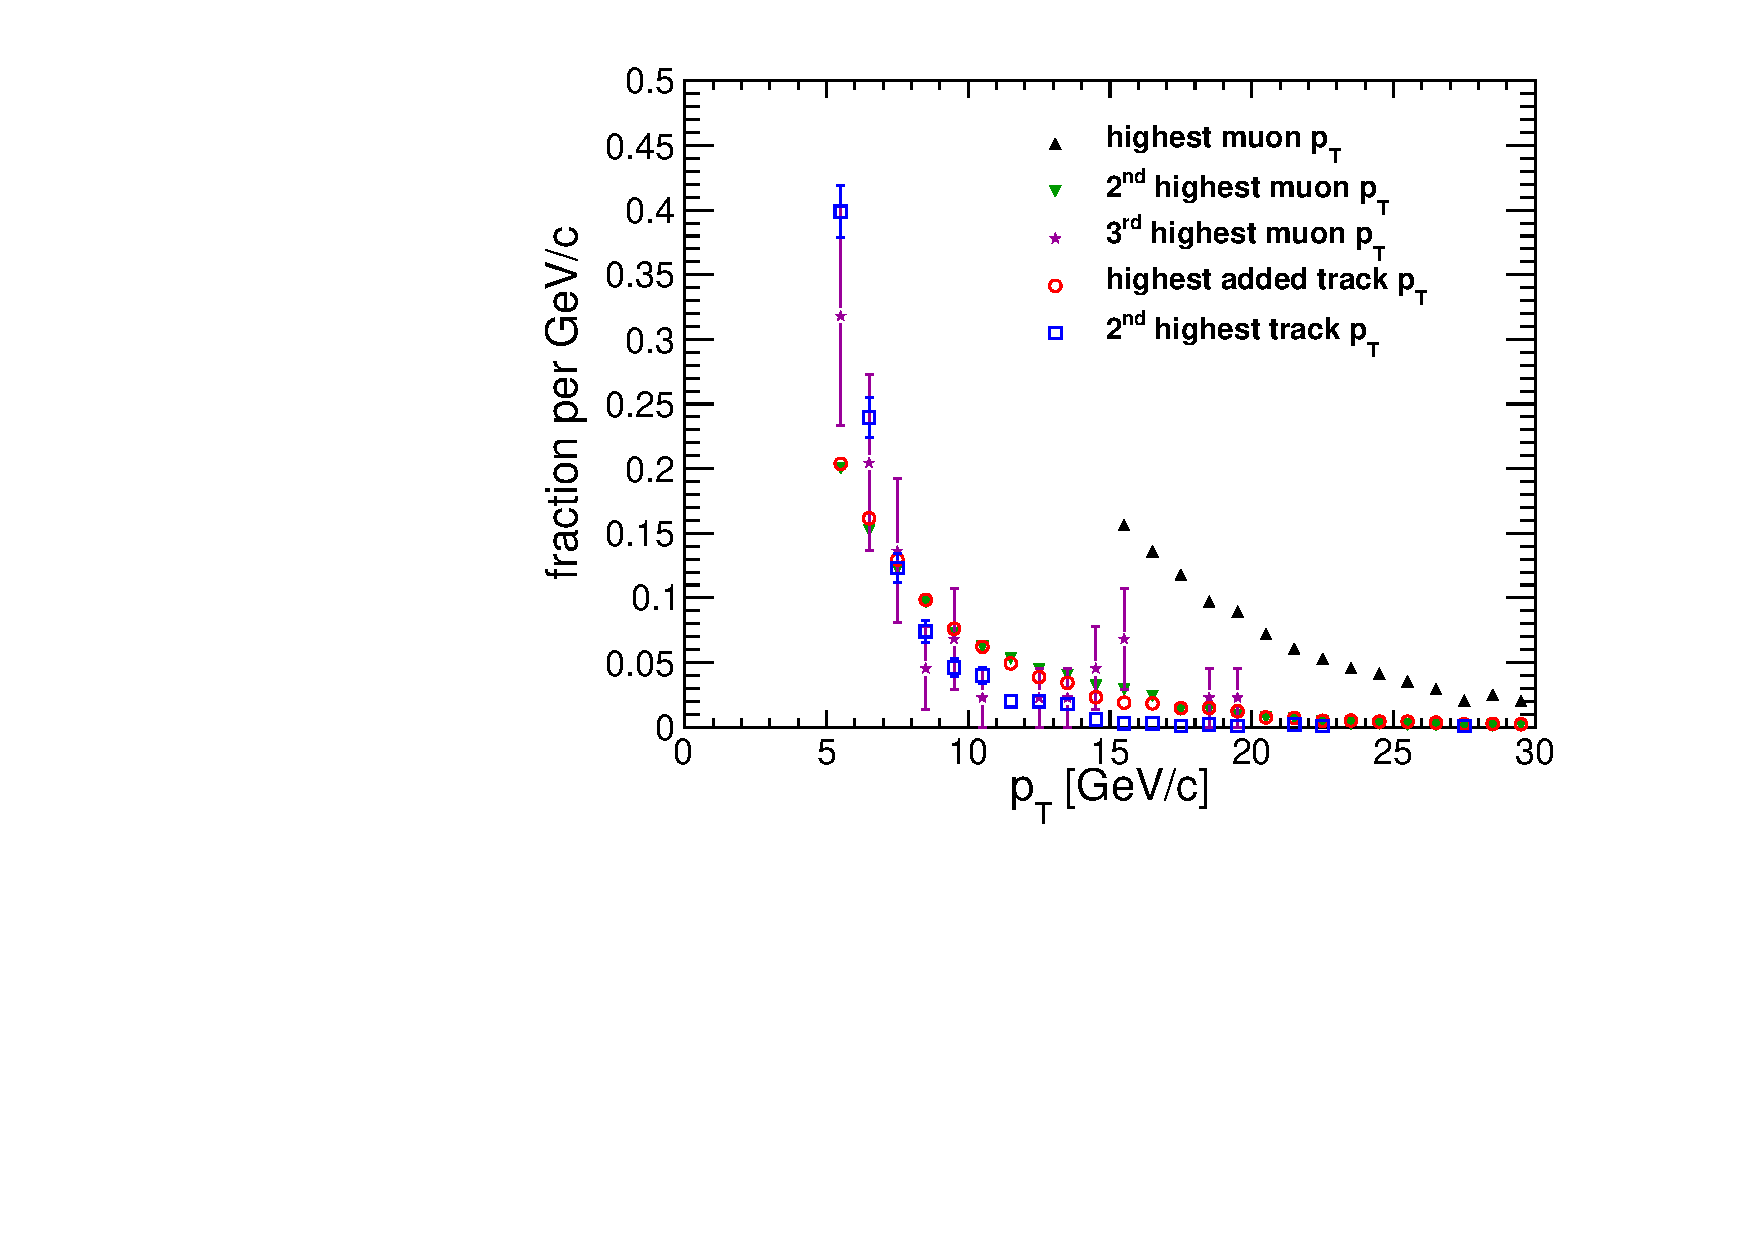
\includegraphics[width=0.5\linewidth]{PLOTS/support_mujetplustracks_ptspectra.pdf}
\end{center}

\caption{Momentum distributions of muons and extra tracks in a sample
  where random tracks have been added to mu-jets.  Only the
  highest-$p_T$ muon is biased (by the trigger
  requirement). \label{fig:support_mujetplustracks_ptspectra}}
\end{figure}

The background-enriched sample is the set of dimuons with two extra
tracks and zero net charge, and the control sample is the set of
three-muon mu-jets with one extra track and zero net charge.
Figure~\ref{fig:backgroundEnriched_fakes} shows a fit to the
background-enriched sample and its overlay on the control sample.  The
fit ansatz is Eqn.~\ref{eqn:bkgnd_shape} with $f_\omega$, $f_\phi$,
$f_{\psi'}$, and $f_m$ fixed to the values obtained in
Fig.~\ref{fig:backgroundEnriched_highpt} (resonances are dwarfed by
continuum shape).  To demonstrate the universality of the fake dimuon
shape, the Monte Carlo distribution of fakes and decays-in-flight in
dimuons is overlaid.

\begin{figure}
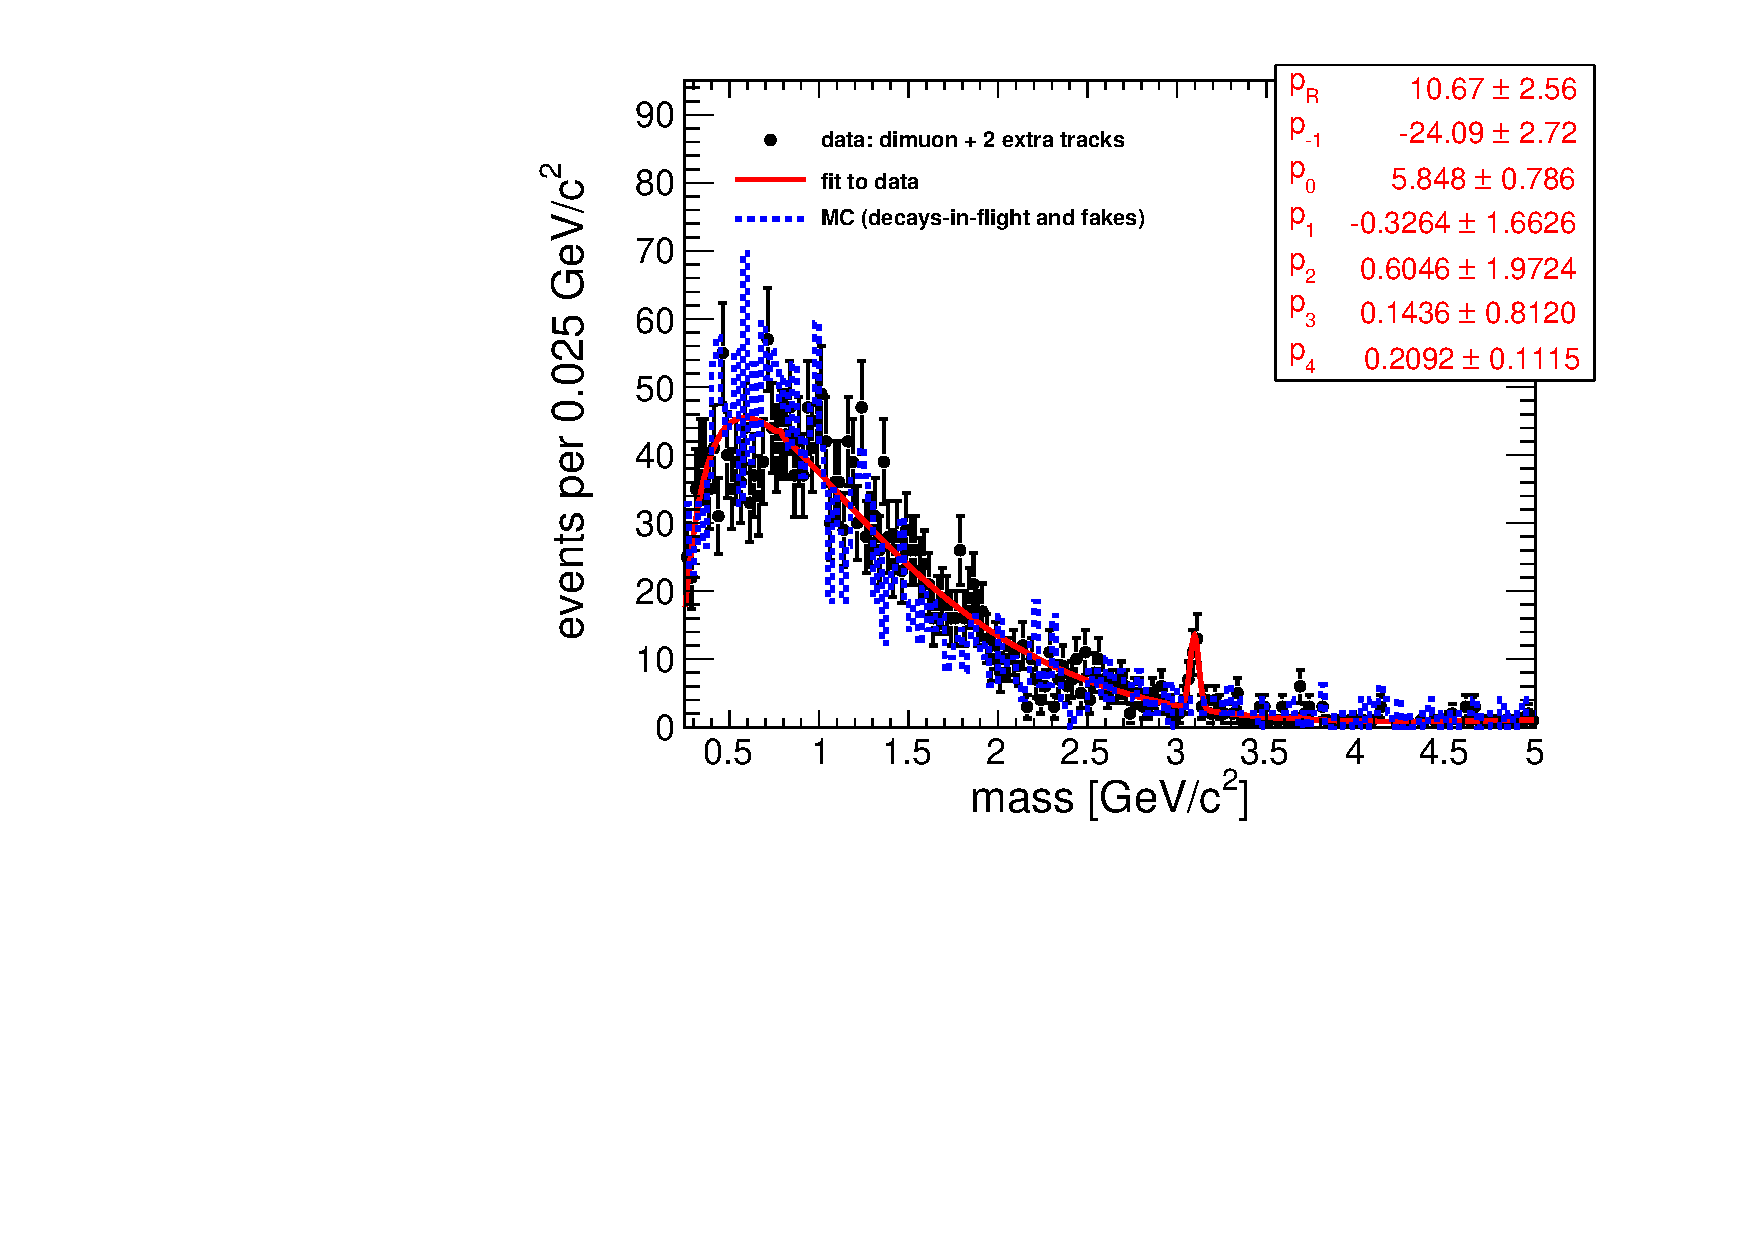
\includegraphics[width=0.5\linewidth]{PLOTS/fullscale-backgroundEnriched_fakes.pdf}
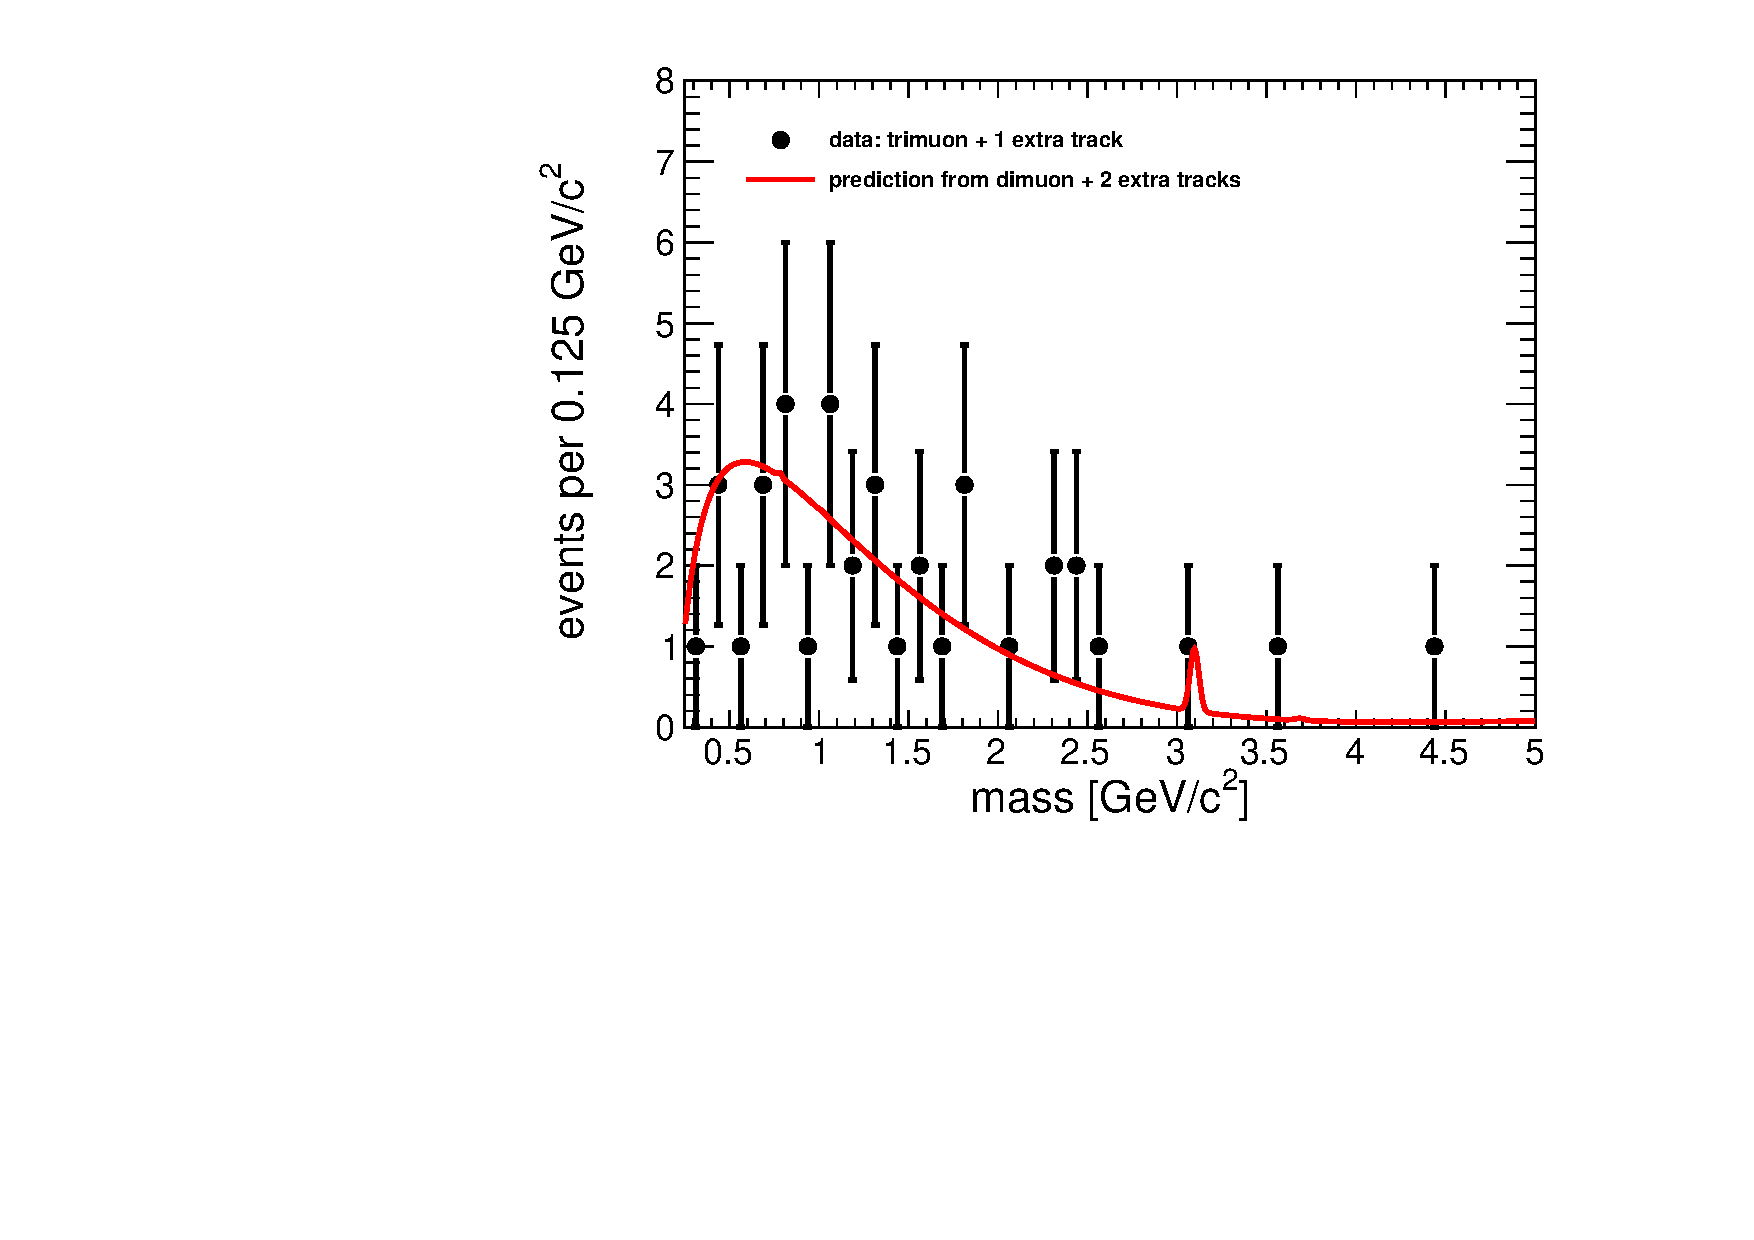
\includegraphics[width=0.5\linewidth]{PLOTS/fullscale-control_fakes.pdf}

\caption{Left: fundamental dimuon distribution from neutral two muon
  plus two extra track mu-jets.  Right: same for neutral three muon plus
  one extra track mu-jets.  Blue distribution is fake and
  decay-in-flight dimuons in Monte Carlo. \label{fig:backgroundEnriched_fakes}}
\end{figure}

As an additional control region, closer to the signal, we show the 2-D
mass distribution of fundamental dimuon masses in four-muon mu-jet
events (Fig.~\ref{fig:quadmu_wholecontrol}).  The signal region along
the diagonal is blinded by a strip that is 5-$\sigma$ wide in detector
resolution, to hide a potential discovery before finalizing the
procedure.  Only one event is observed in the off-diagonal region,
consistent with a simple back-of-the-envelope scaling: the ratios of
two muons plus two extra tracks ($N_{2+2}$), three muons plus one
extra track ($N_{3+1}$), and four muons with no extra tracks
($N_{4+0}$) are as follows:
\begin{equation}
\frac{N_{3+1}}{N_{2+2}} = 0.014 \mbox{ and } \frac{N_{4+0}}{N_{3+1}} = 0.03.
\end{equation}
The single observed event has fundamental dimuon masses of 0.8 and
1.0~GeV/$c^2$, in the bulk of the predicted distribution
(Fig.~\ref{fig:backgroundEnriched_fakes}).  Three of its four muons
have only two segments each, though their trajectories all pass
through four stations.  The pattern of segments suggest only two real
muons.

\begin{figure}
\begin{center}
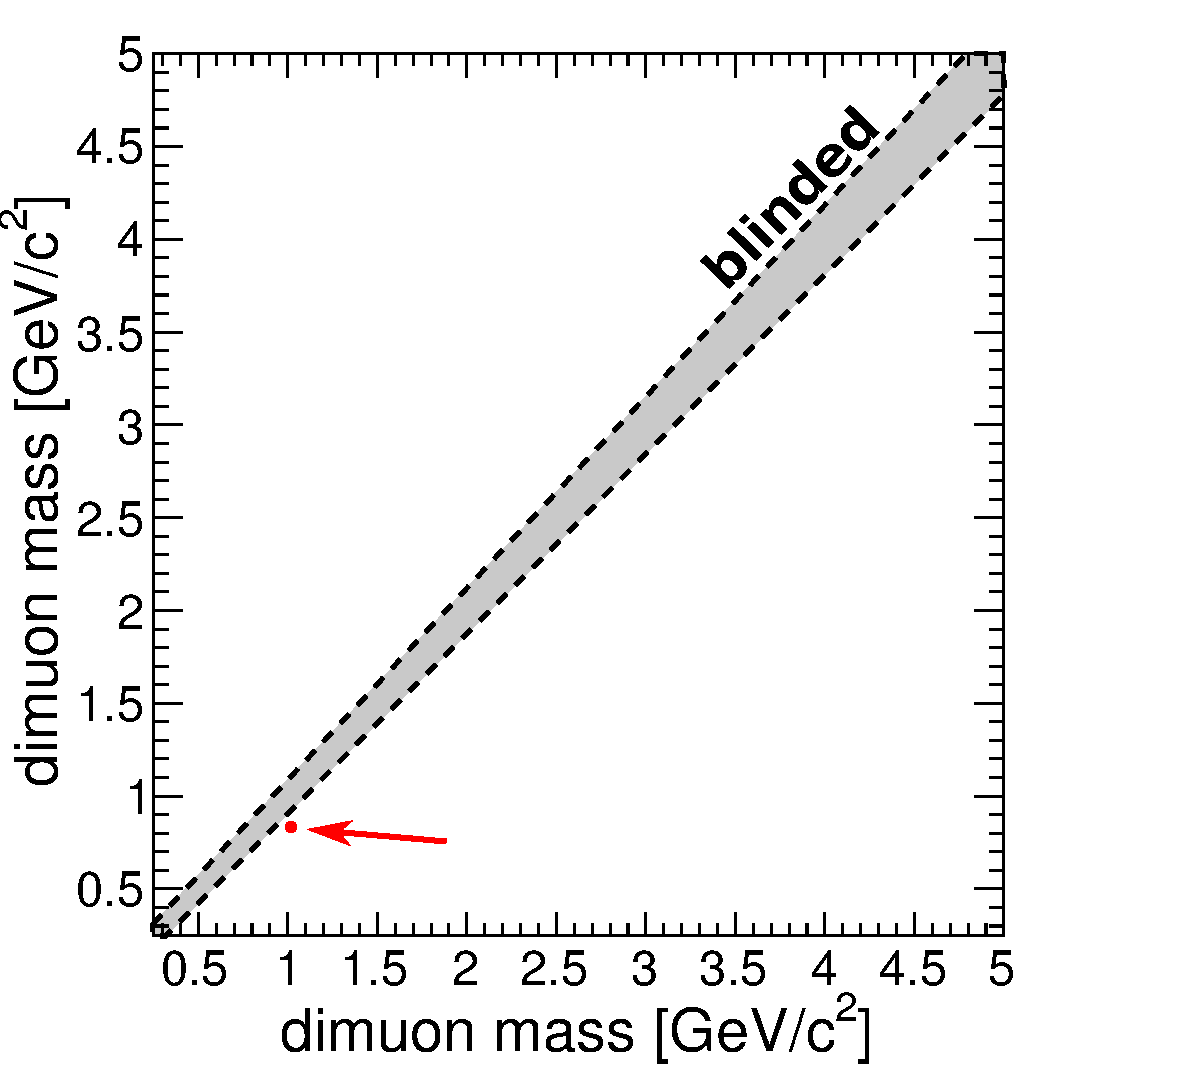
\includegraphics[height=6.5 cm]{PLOTS/data_quadmu_wholecontrol.pdf} \hspace{0.5 cm}
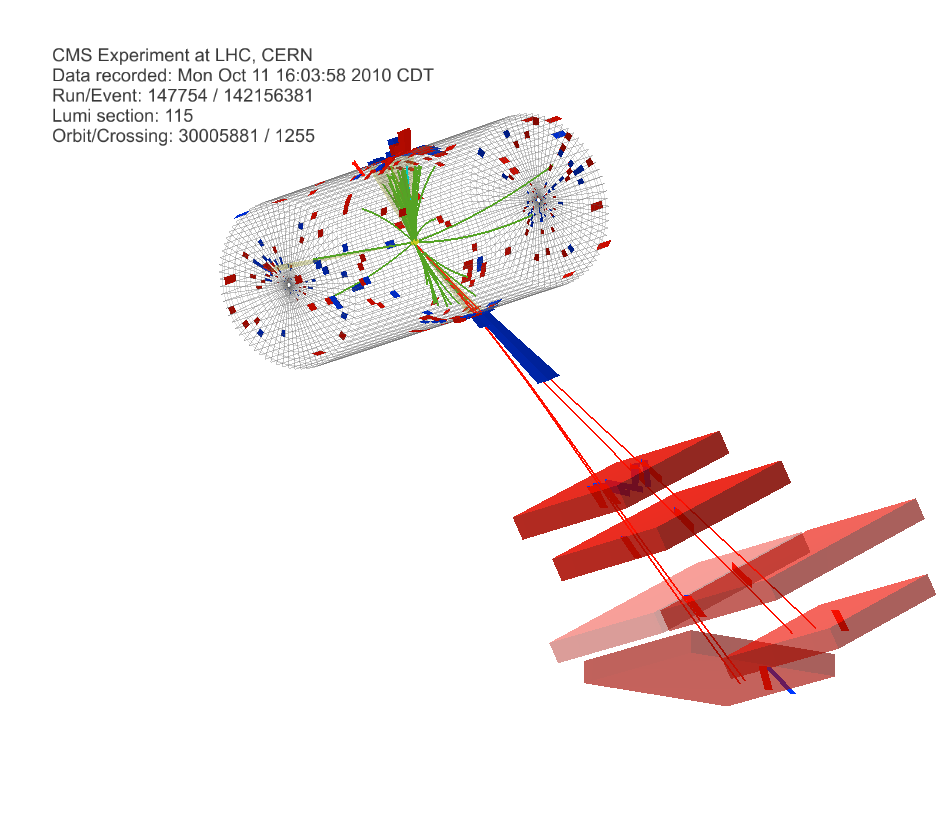
\includegraphics[height=6.5 cm]{PLOTS/quadmu_control_eventdisplay.png}
\end{center}

\caption{Left: fundamental dimuon-dimuon mass plane for signal region
  (a-2) with the strip along the diagonal blinded (5-$\sigma$ in
  detector resolution).  Right: a display of the single event
  surviving cuts. \label{fig:quadmu_wholecontrol}}
\end{figure}

\subsection{Mass template for (b-1): events with two dimuons}

The (b-1) signal region consists of events with two dimuons, a
signature that is predominantly produced in the Standard Model by
$b\bar{b}$ with both $b$-quarks decaying to $\mu\mu X$.  As such, the
background-enriched samples should be $b\bar{b}$.  The $b\bar{b}$ cuts
defined in Eqn.~\ref{eqn:bbcuts} yield a nearly pure sample of
$b\bar{b} \to \mu\mu X$ when applied to dimuons
(Fig.~\ref{fig:support_mass}).  In
Fig.~\ref{fig:support_bbbarcut_efficiency}, we show that they also do
not distort the $b\bar{b}$ dimuon mass distribution, so we use
this distribution as a background-enriched template.

\begin{figure}
\begin{center}
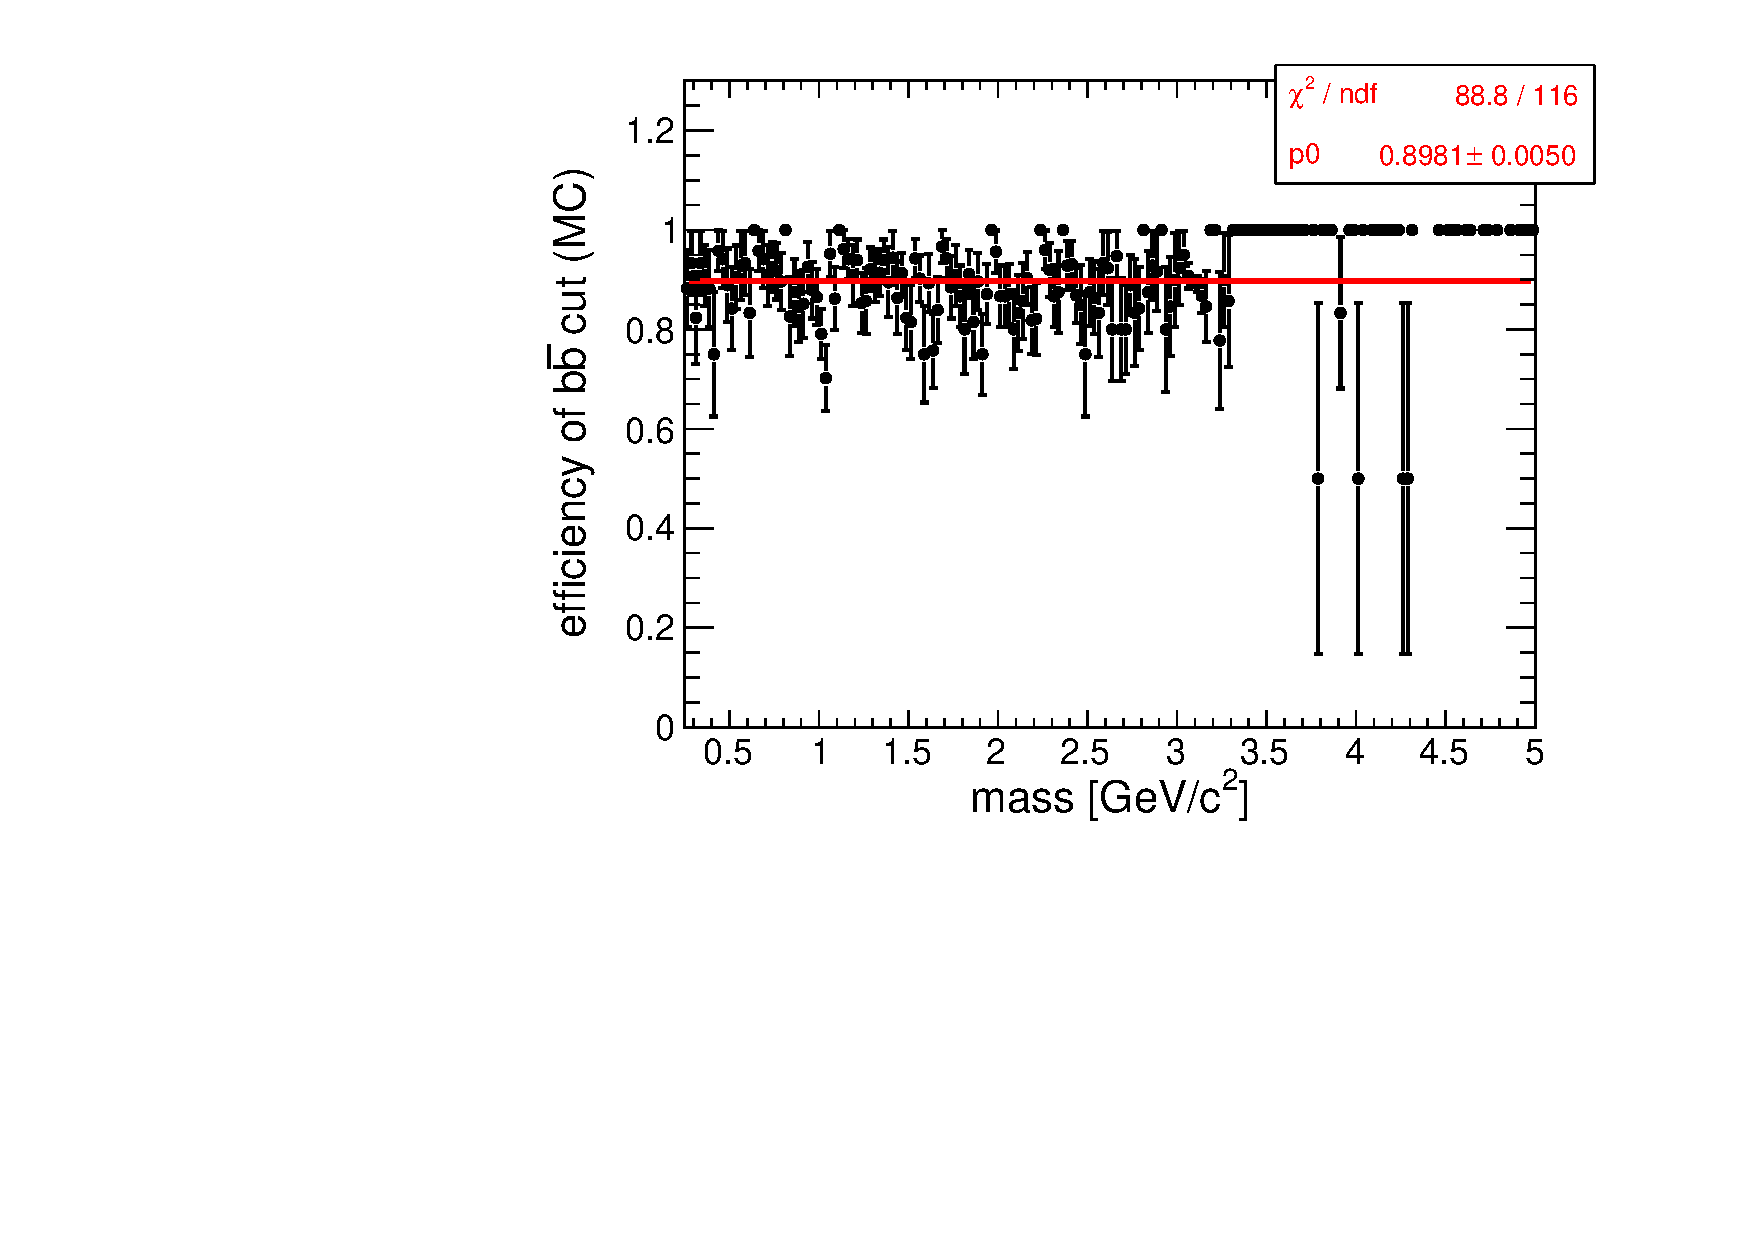
\includegraphics[width=0.6\linewidth]{PLOTS/support_bbbarcut_efficiency.pdf}
\end{center}

\caption{Efficiency of the $b\bar{b}$ cut for simulated $b\bar{b}$
  events, demonstrating that the efficiency is constant, so the
  $b\bar{b}$ cuts do not introduce a shape bias. \label{fig:support_bbbarcut_efficiency}}
\end{figure}

Only one of the two dimuons in the (b-1) signal region needs to
contain a muon satisfying the trigger, which implies a minimum $p_T$
of 20~GeV/$c$ and a direction that points into the barrel of the muon
system ($|\eta| \lesssim 0.9$).  Since the other dimuon does not need
to satisfy the trigger, its minimum $p_T$ is 10~GeV/$c$ and it can
point anywhere in the muon system ($|\eta| \lesssim 2.4$).  The
difference in $p_T$ threshold modifies the mass spectrum, so the
``other dimuon'' mass template must be derived from a
background-enriched sample without biasing the dimuon kinematics with
the trigger.  To do this, we use events with one dimuon and one extra
muon.  The third muon is required to satisfy the trigger, freeing the
dimuon from this constraint.  Three-muon events with a small angle
between two of the muons are predominantly $b\bar{b}$ with one
$b$-quark decaying to $\mu\mu X$ and the other to $\mu X$.

The asymmetry between triggered dimuon and other dimuon introduces
another complication: in some double-dimuon events, both dimuons
satisfy the trigger.  In such cases, we assign the ``triggered
dimuon'' and the ``other dimuon'' labels randomly.  This does not bias
the triggered dimuon distribution, but the part of the other dimuon
phase space that would satisfy the trigger is depleted by a factor of
two.  We want the mass templates to reflect this, so we apply the same
bias to the corresponding background-enriched sample.  In the dimuon
plus third muon sample, we weight events in which the dimuon could
have triggered the event by a factor of 1/2.
Figure~\ref{fig:simulation_pteta} shows the results of a toy Monte
Carlo demonstrating this effect.

\begin{figure}
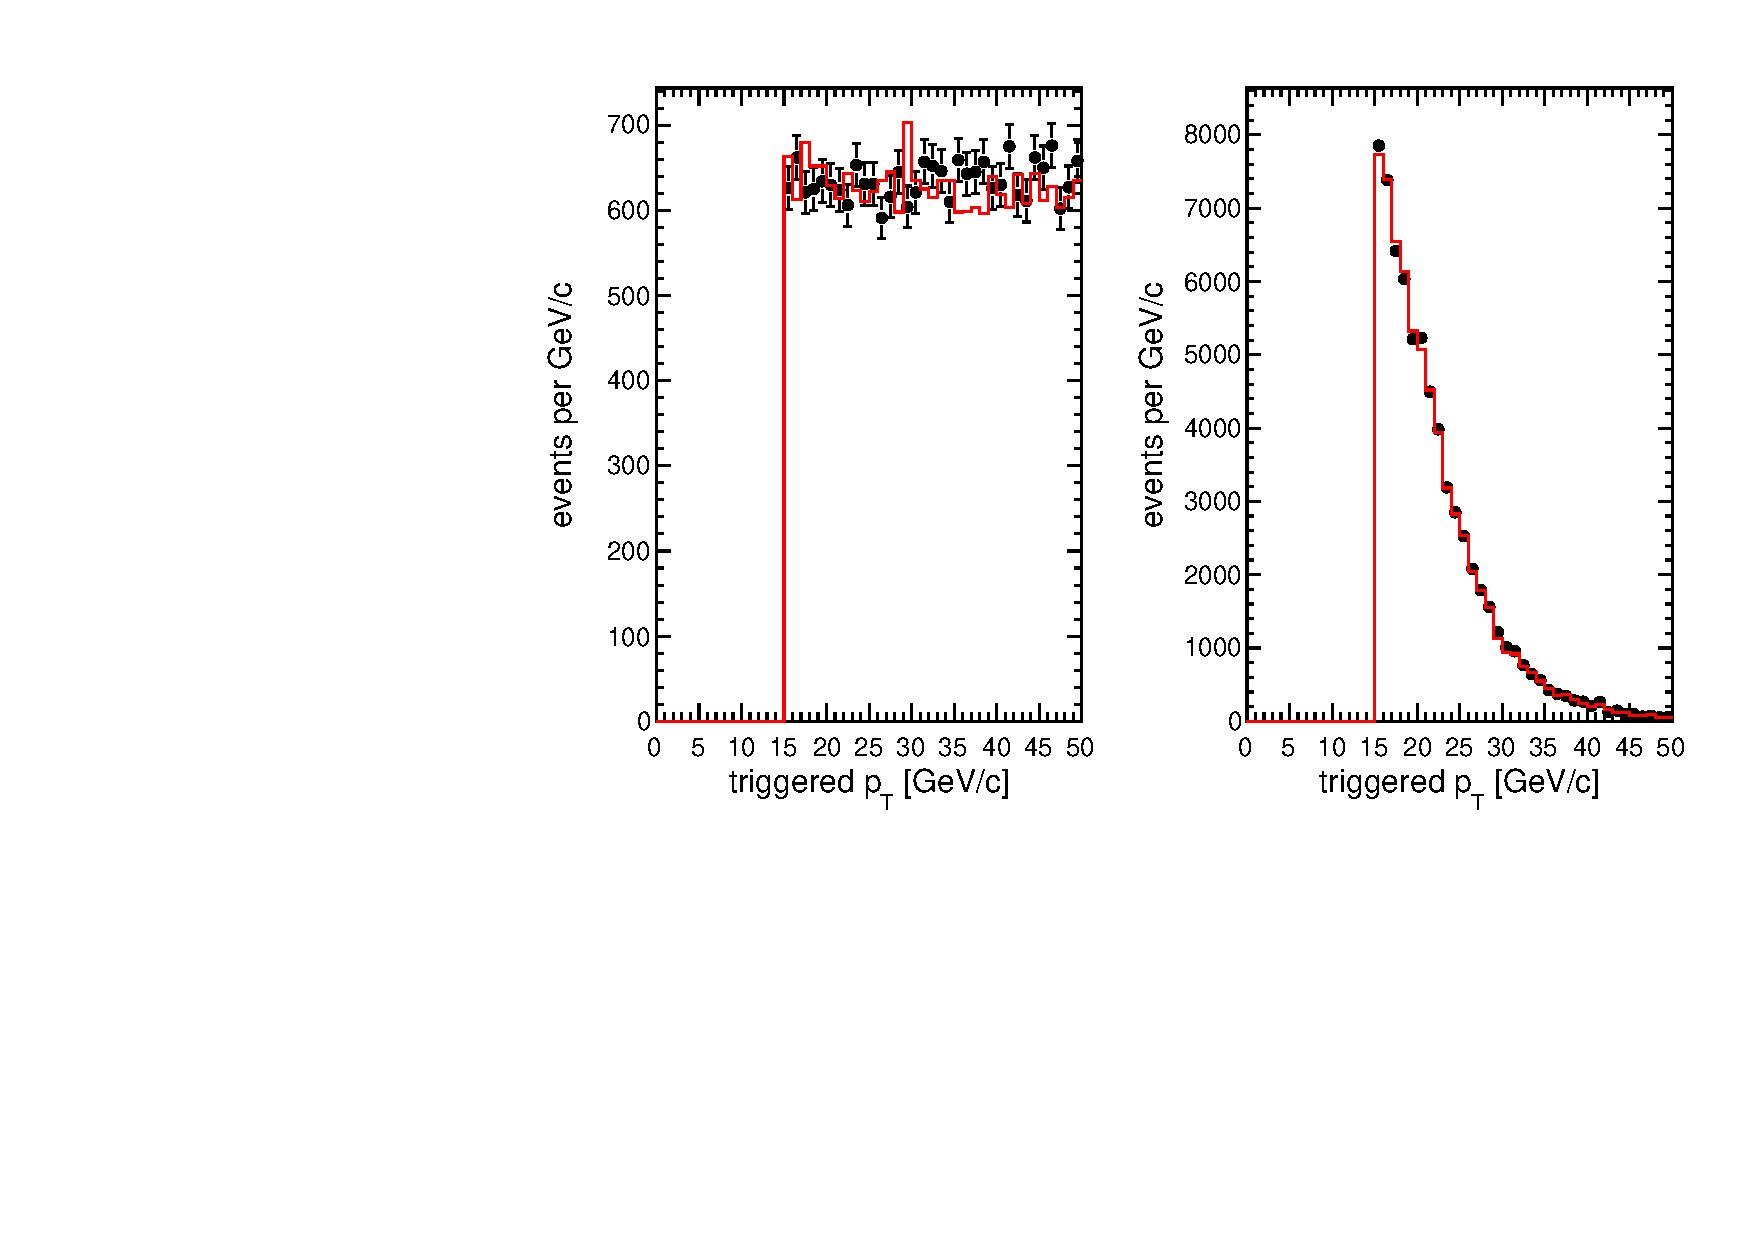
\includegraphics[width=0.47\linewidth]{PLOTS/simulation_triggeredpt.pdf} \hfill
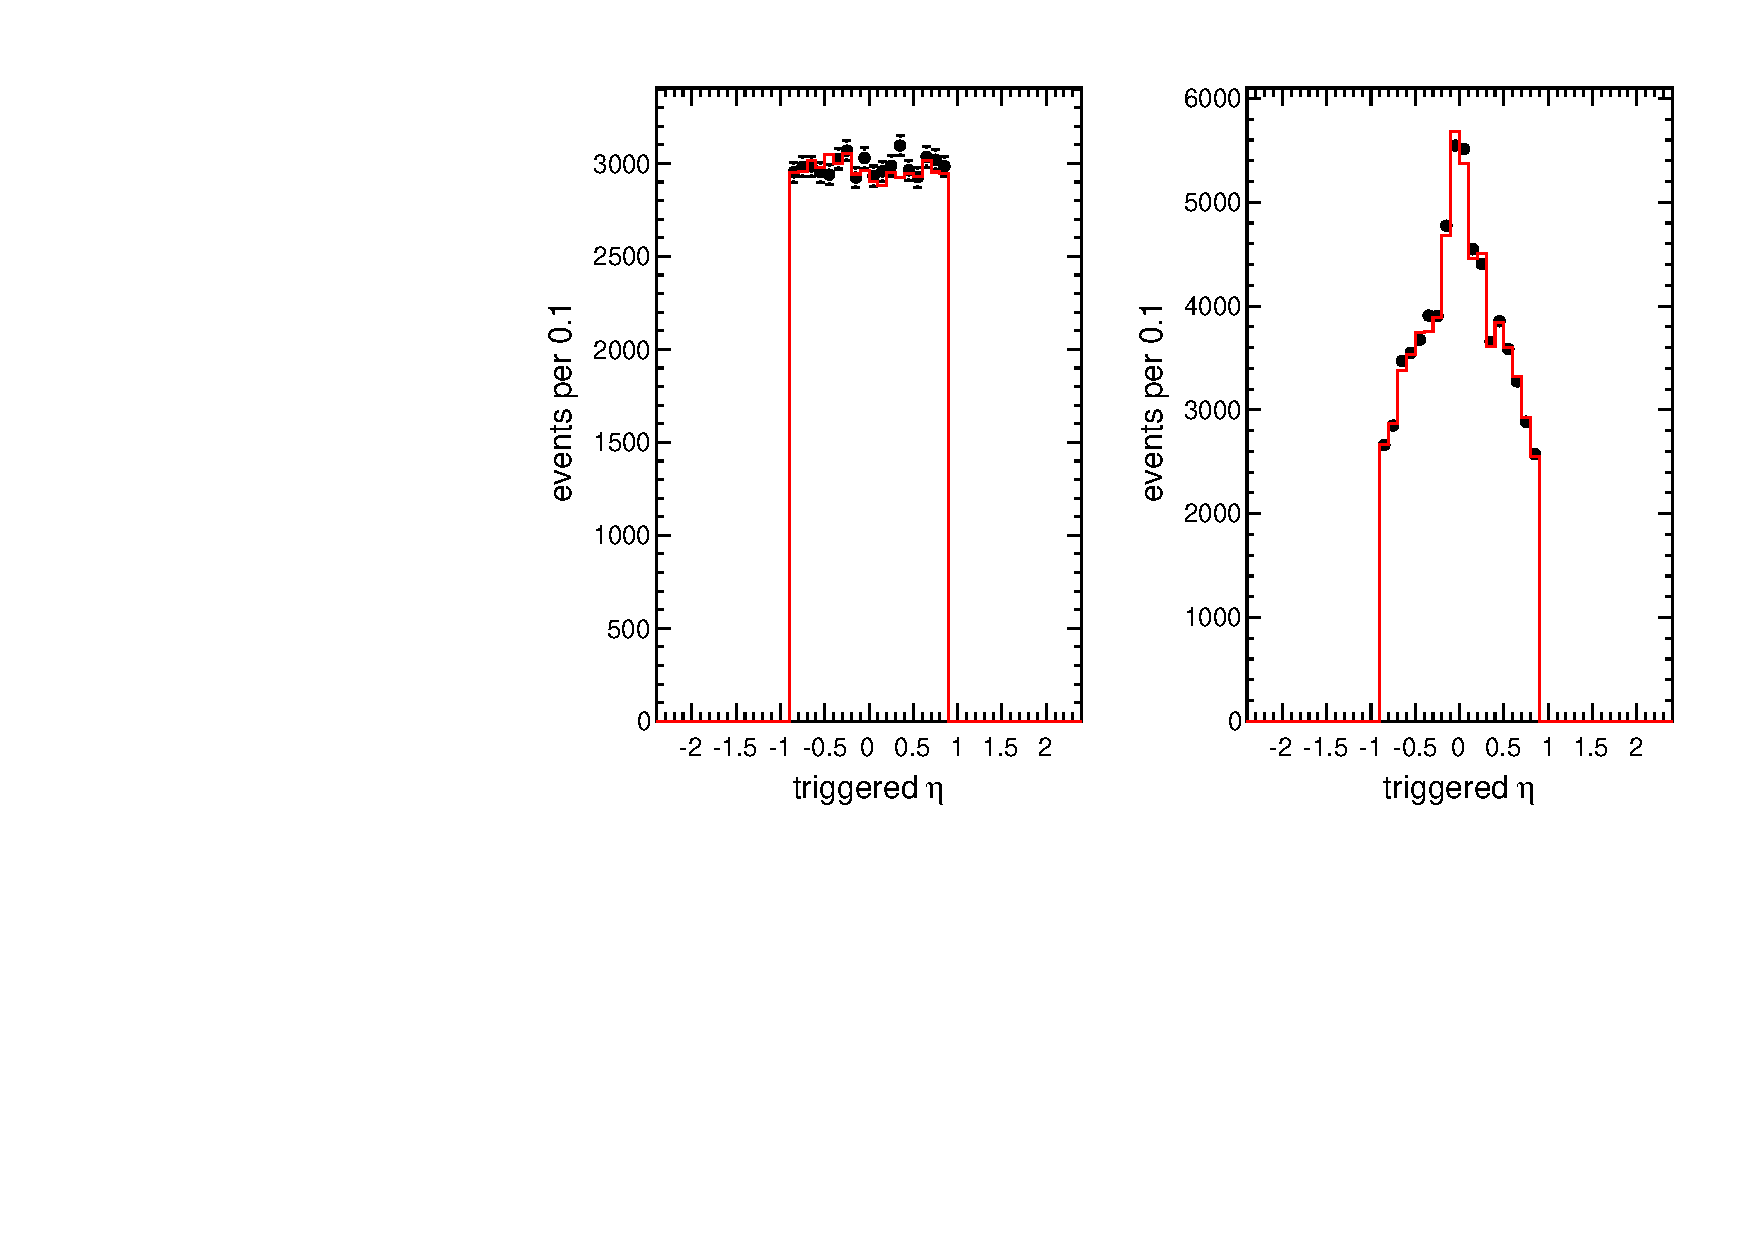
\includegraphics[width=0.47\linewidth]{PLOTS/simulation_triggeredeta.pdf}

\vspace{0.75 cm}
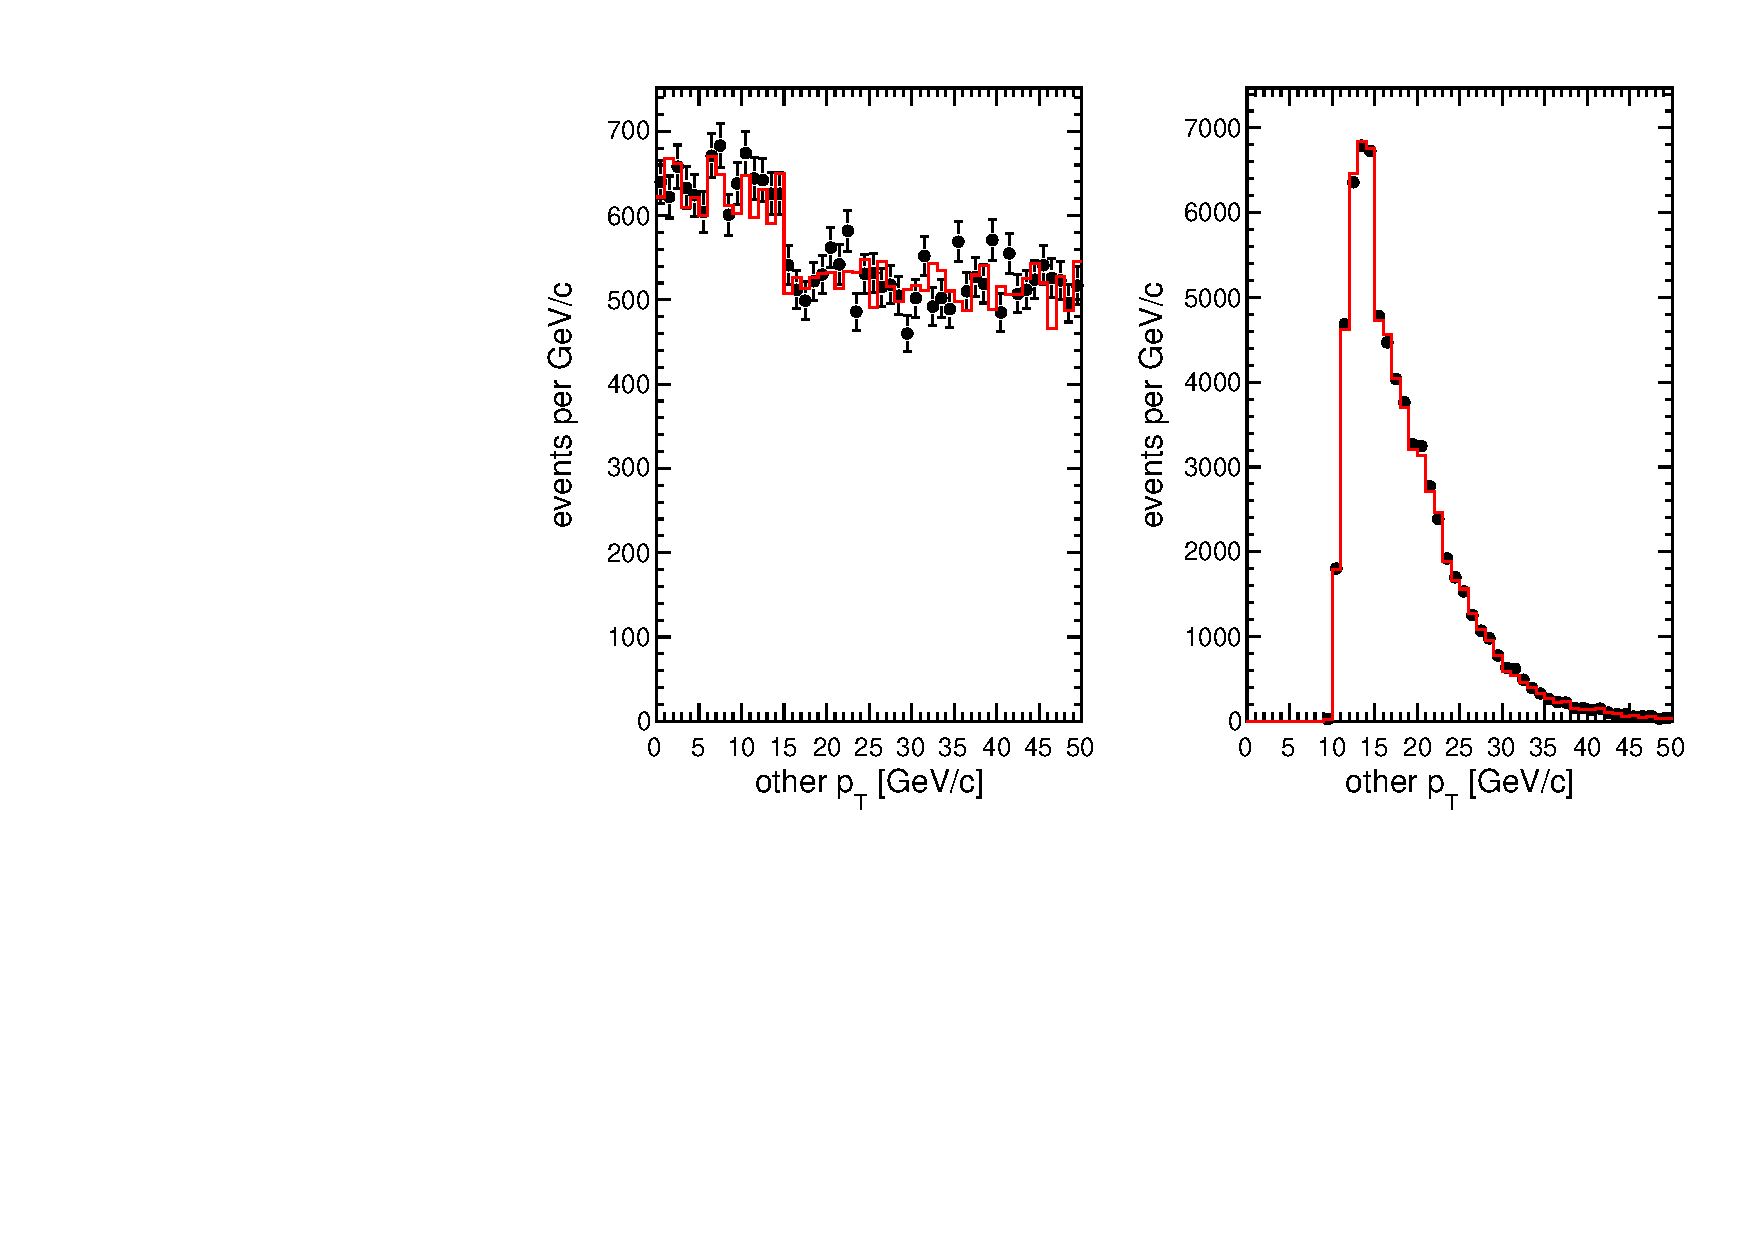
\includegraphics[width=0.47\linewidth]{PLOTS/simulation_otherpt.pdf} \hfill
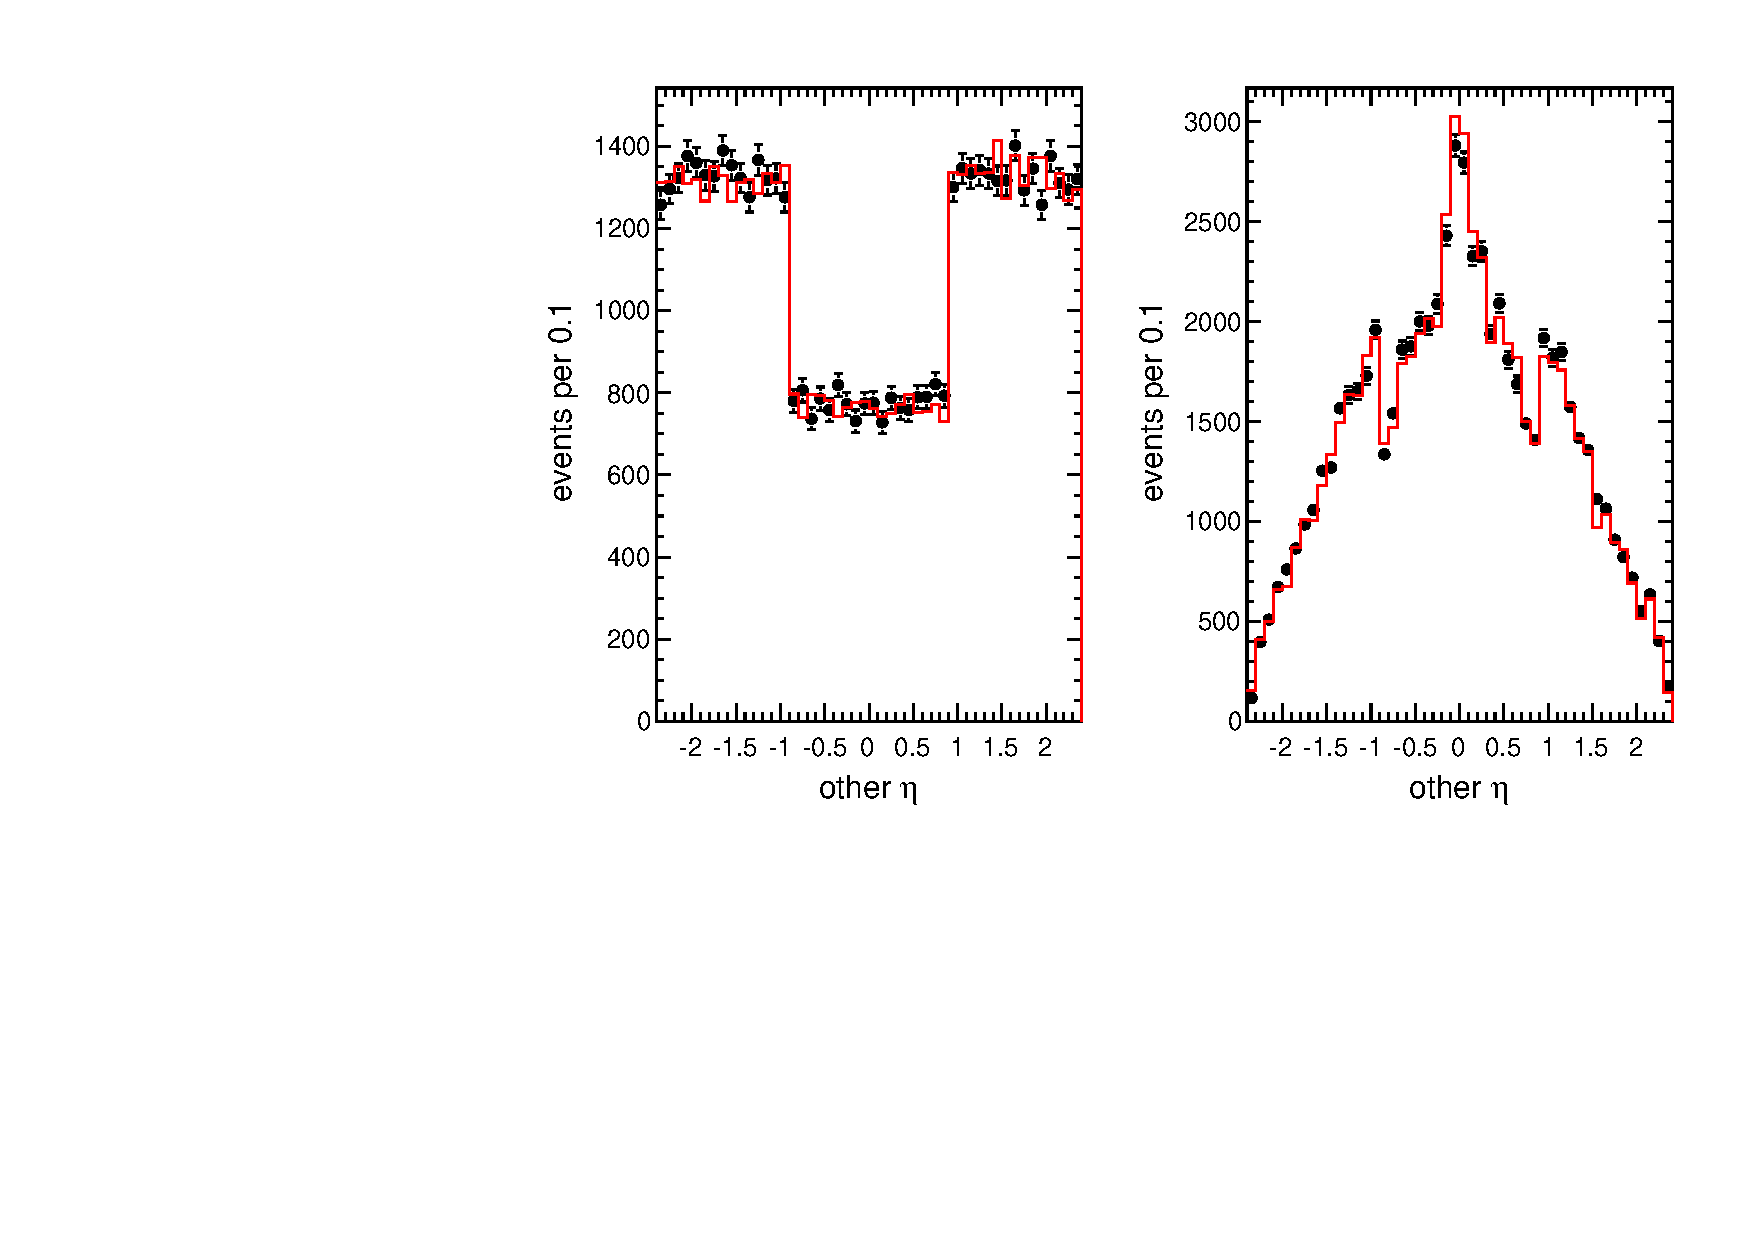
\includegraphics[width=0.47\linewidth]{PLOTS/simulation_othereta.pdf}

\caption{Toy Monte Carlo simulation of backgrounds in the dimuon-dimuon sample
  (black points), extrapolated from single-dimuons and
  dimuon-plus-muon background-enriched samples (red lines).  In each pair of plots, the
  left is a simplified model with uniform $p_T$ and $\eta$
  distributions and the right is a model with realistic $p_T$ and
  $\eta$ distributions.  The ``other dimuon'' distribution is
  depleted in the signal region, but the background-enriched sample
  is weighted to have the same distribution. \label{fig:simulation_pteta}}
\end{figure}

Fits to both background-enriched samples are presented in
Fig.~\ref{fig:backgroundEnriched_massCF}.  The dimuons with $b\bar{b}$
cuts sample (for triggered dimuons) is fitted to
Eqn~\ref{eqn:bkgnd_shape} with only $p_{-1}$ fixed to zero, and the
low-statistics dimuons plus third muon sample (for other dimuons) is
fitted to the same ansatz with $f_\omega$, $f_\phi$, $f_{\psi'}$, and
$f_m$ fixed to the values determined by the first fit.  Monte Carlo
distributions for the corresponding $b\bar{b} \to 2\mu \, 2\mu \, X$ signal
region are overlaid to show the difference between the data-driven
template shape and a template shape that could have been derived from
Monte Carlo.

\begin{figure}
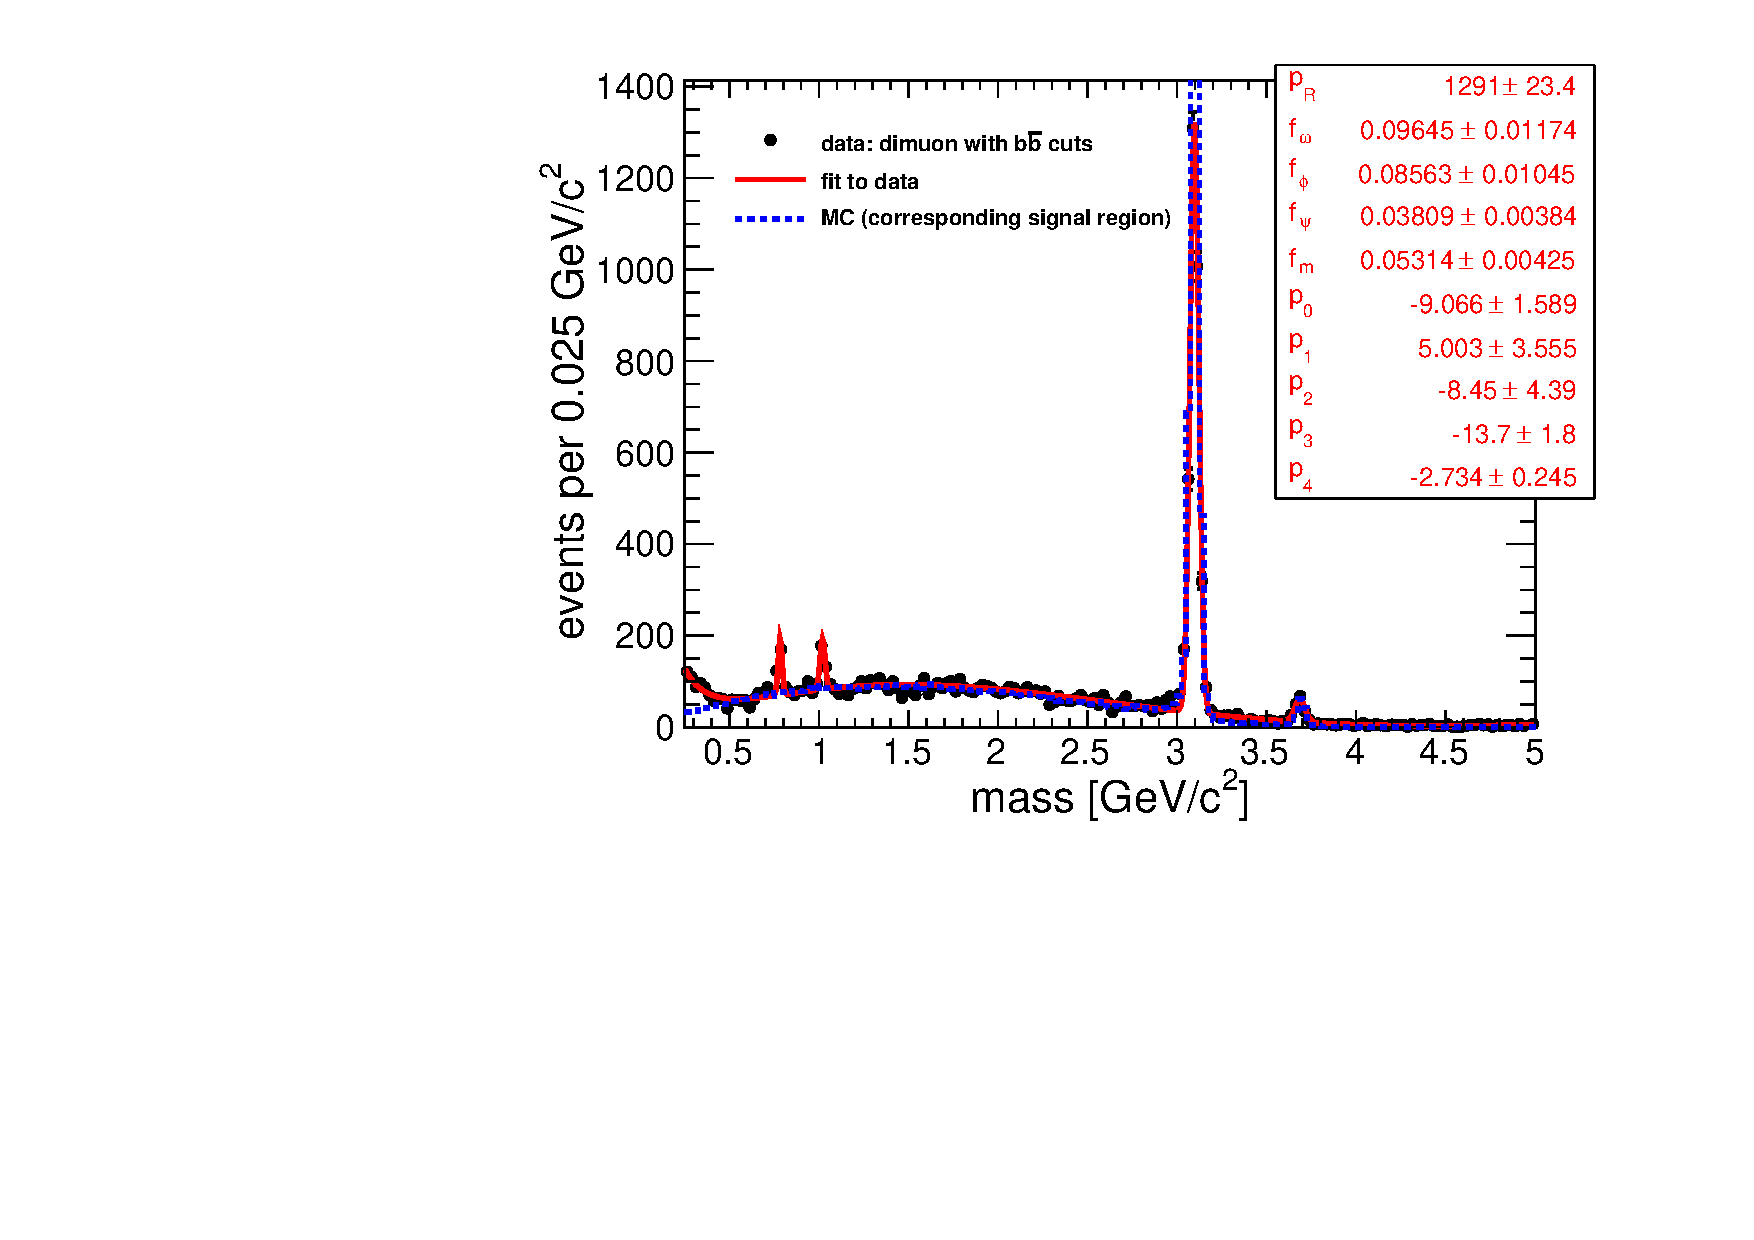
\includegraphics[width=0.5\linewidth]{PLOTS/fullscale-backgroundEnriched_massC.pdf}
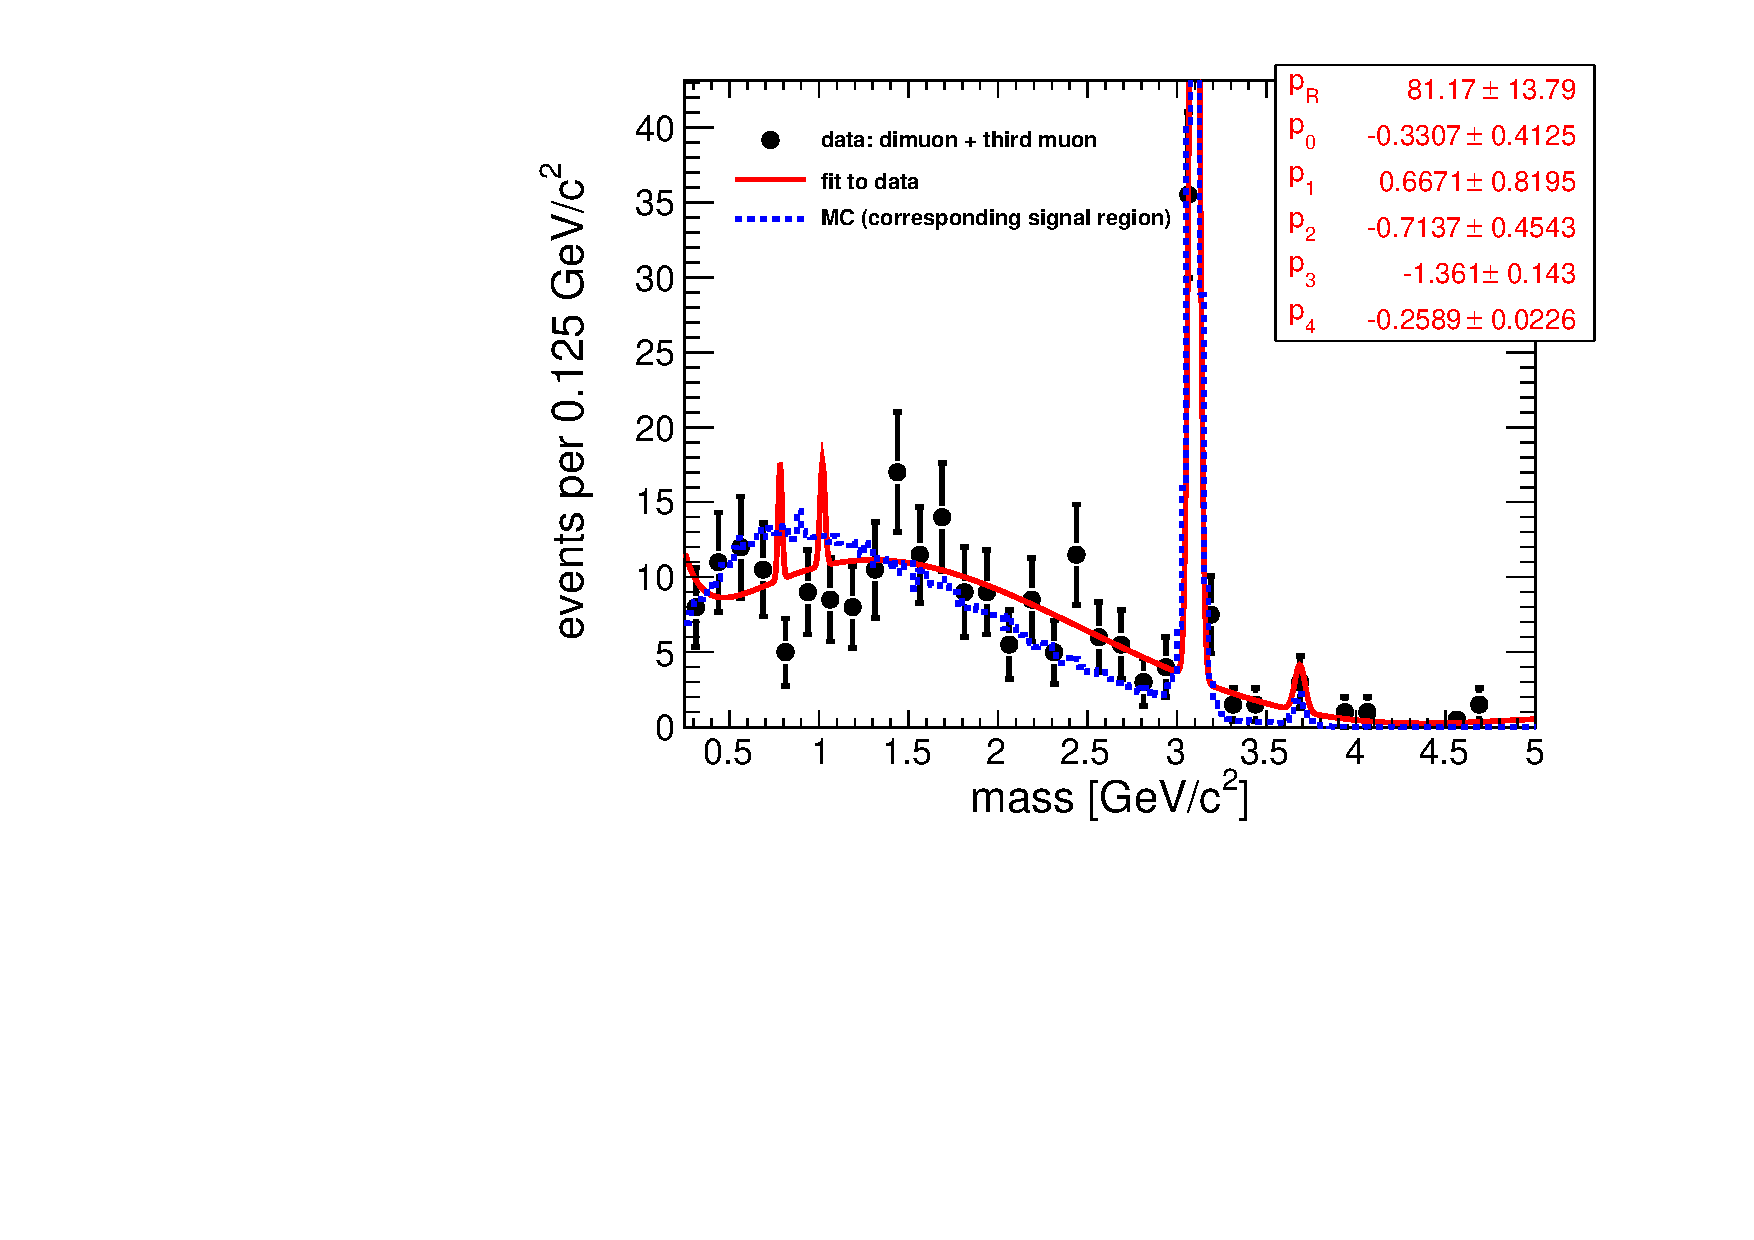
\includegraphics[width=0.5\linewidth]{PLOTS/fullscale-backgroundEnriched_massF.pdf}

\caption{Left: dimuons with $b\bar{b}$ cuts (background-enriched
  region for triggered dimuon).  Right: dimuons plus extra muon
  (background-enriched region for other dimuon).  Both are overlaid
  by template shape fits and Monte Carlo samples for the
  corresponding signal region. \label{fig:backgroundEnriched_massCF}}
\end{figure}

The control region for (b-1) is the off-diagonal part of the
dimuon-dimuon mass plane.  Figure~\ref{fig:dimudimu_wholecontrol}
shows this plane with a 5-$\sigma$ strip along the diagonal blinded.
Only ten events were observed, which is consistent with
back-of-the-envelope scaling of the $b\bar{b} \to 2\mu X$ sample:
$12\,841$ events times 0.2\% $\mathcal{B}(b \to 2\mu X)$ (EvtGen) = 25
events.  The distribution of these events appears to be consistent
with the shapes of the background-enriched samples and inconsistent
with fake or decay-in-flight distributions
(Fig.~\ref{fig:backgroundEnriched_fakes}).

\begin{figure}
\begin{center}
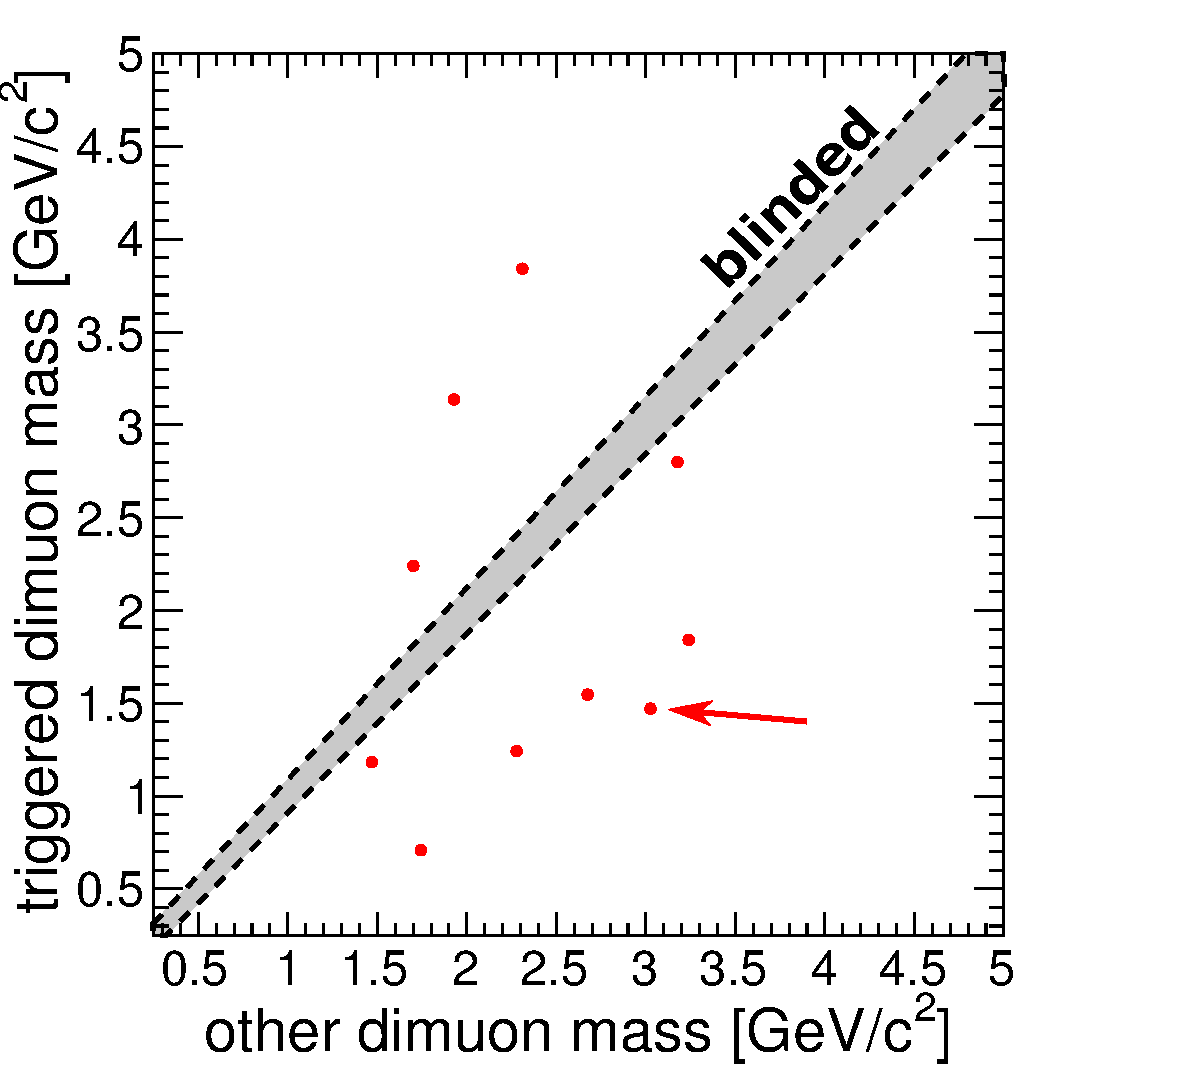
\includegraphics[height=7 cm]{PLOTS/data_dimudimu_wholecontrol.pdf} \hspace{0.5 cm}
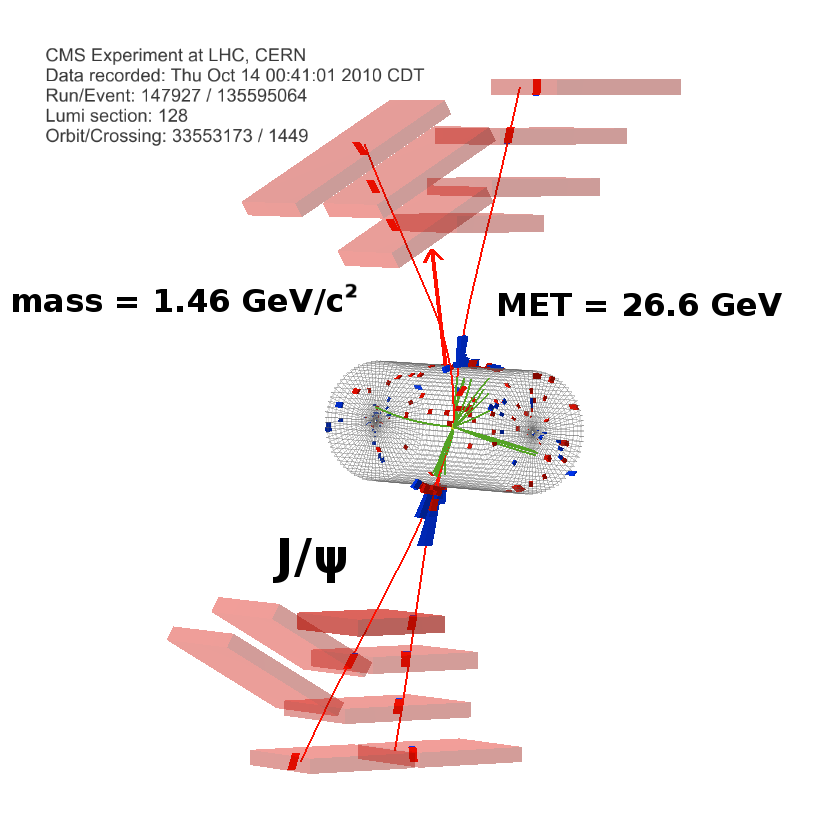
\includegraphics[height=7 cm]{PLOTS/dimudimu_control_eventdisplay.png}
\end{center}

\caption{Left: dimuon-dimuon mass plane for signal region (b-1) with
  the strip along the diagonal blinded (5-$\sigma$ in detector
  resolution).  Right: an event display of a typical event (the one
  indicated by a red arrow in the dimuon-dimuon
  plot.) \label{fig:dimudimu_wholecontrol}}
\end{figure}

The 2-D background shape template is built from a Cartesian product of
the triggered dimuon shape and the other dimuon shape.  To demonstrate
that this is valid, a large Monte Carlo sample of $b\bar{b} \to 2\mu
\, 2\mu \, X$ was generated using Pythia 6 and EvtGen.
Figure~\ref{fig:mc_dimudimu_wholecontrol} shows the rectilinear
structure of the simulated dimuon-dimuon mass plane and projections of
the whole plane overlaid on slices around the $J/\psi$ resonances.

\begin{figure}
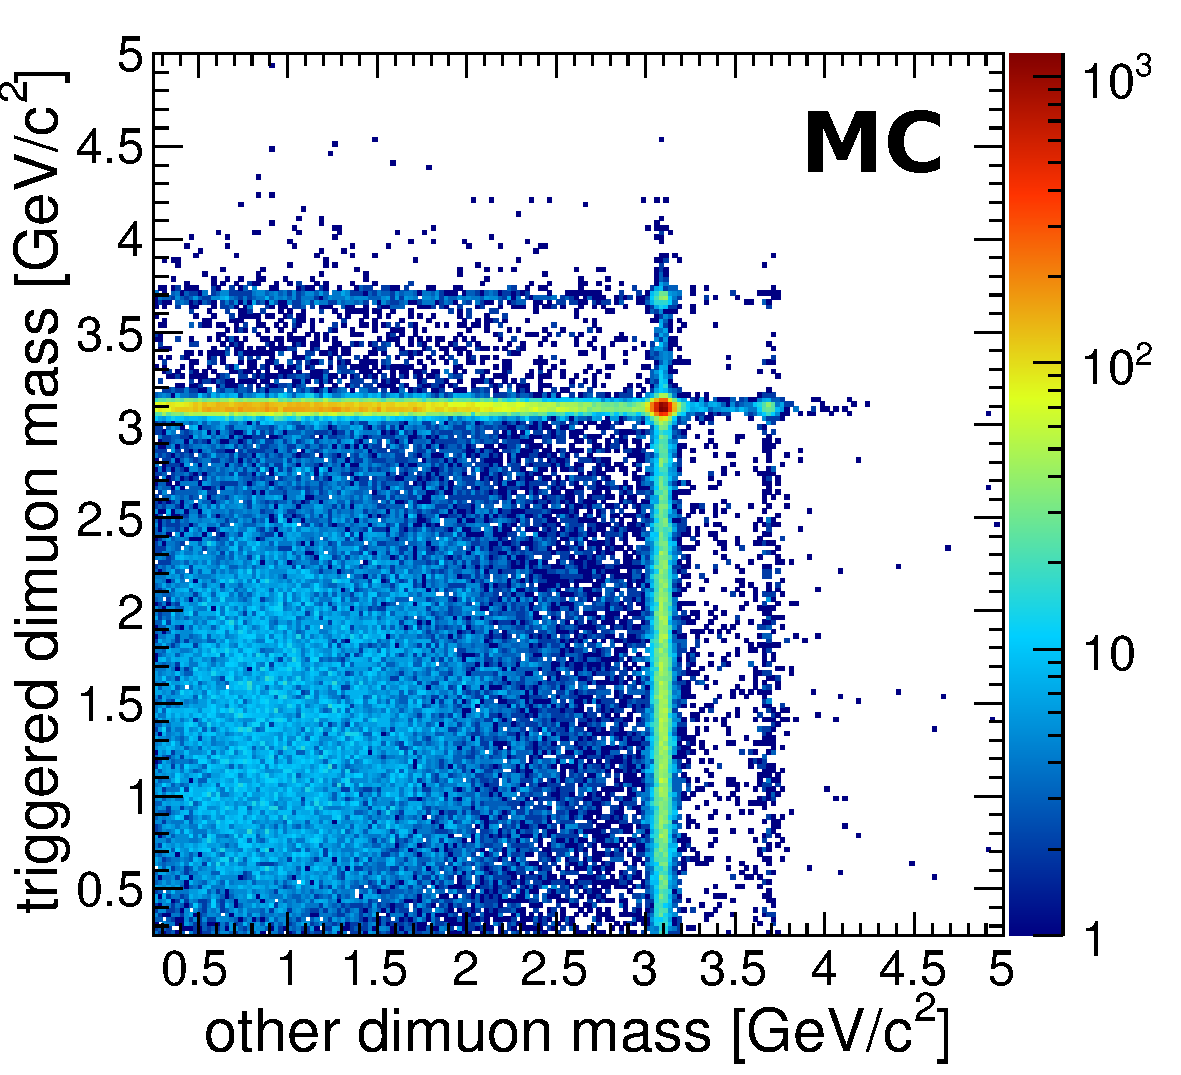
\includegraphics[height=6.2 cm]{PLOTS/mc_dimudimu_wholecontrol.pdf} \hfill
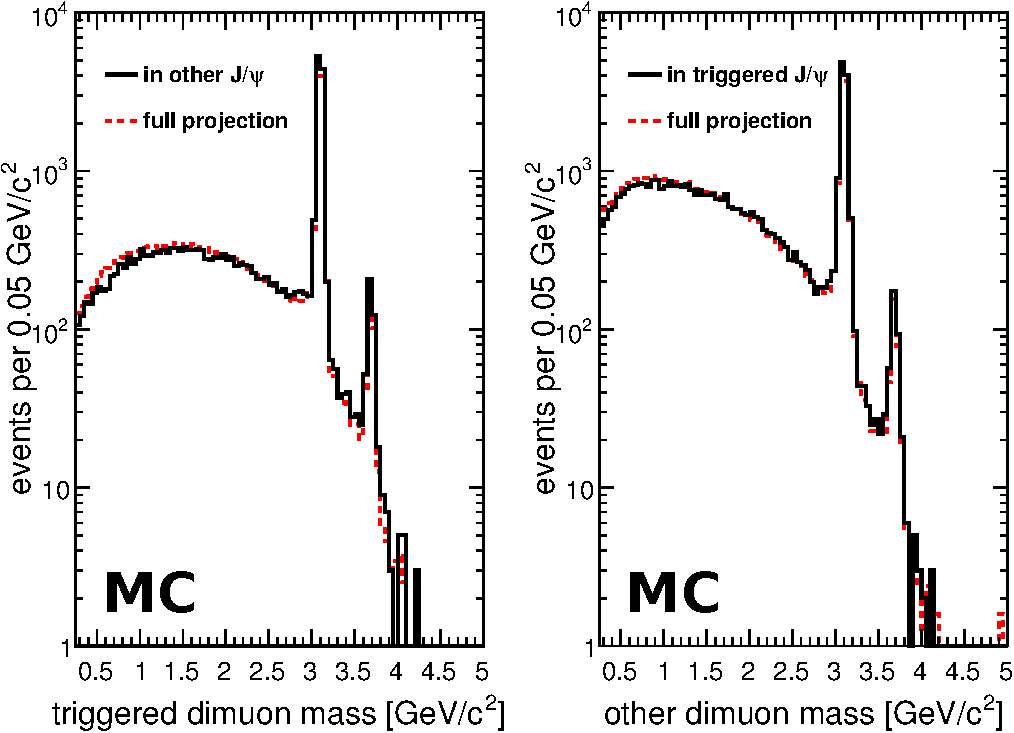
\includegraphics[height=6 cm]{PLOTS/mc_wholecontrolregions_factorize.pdf}

\caption{A Monte Carlo simulation of $b\bar{b} \to 2\mu \, 2\mu \, X$
  events to demonstrate the factorization of background mass
  distributions.  Left: the 2-D distribution.  Right: projected
  distributions in a slice around the $J/\psi$ and the whole
  distribution, normalized to equal areas. \label{fig:mc_dimudimu_wholecontrol}}
\end{figure}

\section{Fits of signal regions}

\subsection{Systematic undertainties}

\subsection{Results}

(mass-peak plots)

\subsection{Limits}

(limit plots)

\section{Cut-flow and limits on benchmark models}

\section{Conclusions}

\appendix

\section{Motivation for reconstruction methods}

\section{Motivation for trigger choice}
\label{sec:motivation_for_trigger_choice}

\end{document}

